\documentclass[11pt]{report}
%% Useful packages
\usepackage[utf8]{inputenc}
\usepackage[a4paper,left=2cm,right=2cm,top=2cm,bottom=2cm]{geometry}
\usepackage{crop,graphicx,amsmath,array,color,amssymb,fancyhdr,lineno,float,booktabs,mhchem}
\usepackage{flushend,stfloats,amsthm,chngpage,times,,lipsum,lastpage,parskip,adjustbox} 
\usepackage{calc,listings,color,wrapfig,tabularx,longtable,multirow,enumitem,commath,siunitx}
\usepackage[table,xcdraw]{xcolor}
%\usepackage[numbers]{natbib}
%\usepackage[subtle]{savetrees}
\usepackage[
  nottoc
  %notlot
  %notlof
]{tocbibind}

\usepackage{hyperref}
\hypersetup{
    colorlinks=true,
    linkcolor=black,
    filecolor=teal,      
    urlcolor=teal,
    citecolor=teal,
    pdftitle={MECH0074 Topic Notes},
    pdfauthor={HD},
    pdfpagemode=FullScreen,
}

\renewcommand\bibname{References}
\usepackage{lineno}
%%%%%%%%%%%%   Header and Footer  %%%%%%%%%%%%%
\pagestyle{fancy}
\fancypagestyle{plain}{%
  \renewcommand{\headrulewidth}{0pt}%
  \fancyhf{}%
  \addtolength{\topmargin}{-2pt}
}

\title{%
  Topic Notes}
\author{HD
}

\begin{document}
\begin{titlepage}

  \newcommand{\HRule}{\rule{\linewidth}{0.5mm}} % Defines a new command for the horizontal lines, change thickness here

  %----------------------------------------------------------------------------------------
  %	LOGO SECTION
  %----------------------------------------------------------------------------------------
  \center
  
\includegraphics[width=5cm]{Title/UCL.png}\\[1cm] % Include a department/university logo - this will require the graphicx package

  %----------------------------------------------------------------------------------------

  \center % Center everything on the page

  %----------------------------------------------------------------------------------------
  %	HEADING SECTIONS
  %----------------------------------------------------------------------------------------

  \textsc{\LARGE University College London }\\[1.5cm] % Name of your university/college
  \textsc{\Large MEng Mechanical Engineering  }\\[0.5cm] % Major heading such as course name
  \textsc{\large MECH0071 Electrical Power Systems and Electrical Propulsion }\\[1.5cm] % Minor heading such as course title

  %----------------------------------------------------------------------------------------
  %	TITLE SECTION
  %----------------------------------------------------------------------------------------
  \makeatletter
  { \huge \textsc \@title}\\[1.5cm] % Title of your document


  %----------------------------------------------------------------------------------------
  %	AUTHOR SECTION
  %----------------------------------------------------------------------------------------

  \begin{minipage}{0.4\textwidth}
    \begin{flushleft} \large
      \emph{Author:}\\
      \@author % Your name
      \\[1.2em]
      %\emph{ID No:}\\
      %0101010 \\[1.2em]
    \end{flushleft}
  \end{minipage}
  ~
  \begin{minipage}{0.4\textwidth}
    \begin{flushright} \large
      \emph{Module coordinator:} \\
      Prof. Richard Bucknall \\[1.2em] % Supervisor's Name
      %\emph{Module teaching team:} \\
      %Dr. Tim Hillel\\ % second marker's name
      %Mr. Umut Lagap
    \end{flushright}
  \end{minipage}\\[2cm]
  \makeatother

  % If you don't want a supervisor, uncomment the two lines below and remove the section above
  %\Large \emph{Author:}\\
  %John \textsc{Smith}\\[3cm] % Your name

  %----------------------------------------------------------------------------------------
  %	DATE SECTION
  %----------------------------------------------------------------------------------------

  {\large \today}\\[2cm] % Date, change the \today to a set date if you want to be precise

  \vfill % Fill the rest of the page with whitespace

\end{titlepage}

\fancyhf{}
\fancyhead[L]{MECH0074}
\fancyfoot[L]{HD}
\fancyfoot[R]{ \bf\thepage\ \rm }%

\newpage
\tableofcontents
\newpage
\listoffigures
\listoftables
\newpage

\part{Extreme Pressure}
\chapter{Materials, Molecules and Chemistry}
\section{Introduction}
\begin{itemize}
	\item Macroscopic response of material depends on their microscopic structure
	\item We need to be able to understand physics from molecular to continuum scales
\end{itemize}
\begin{figure}[H]
	\centering
	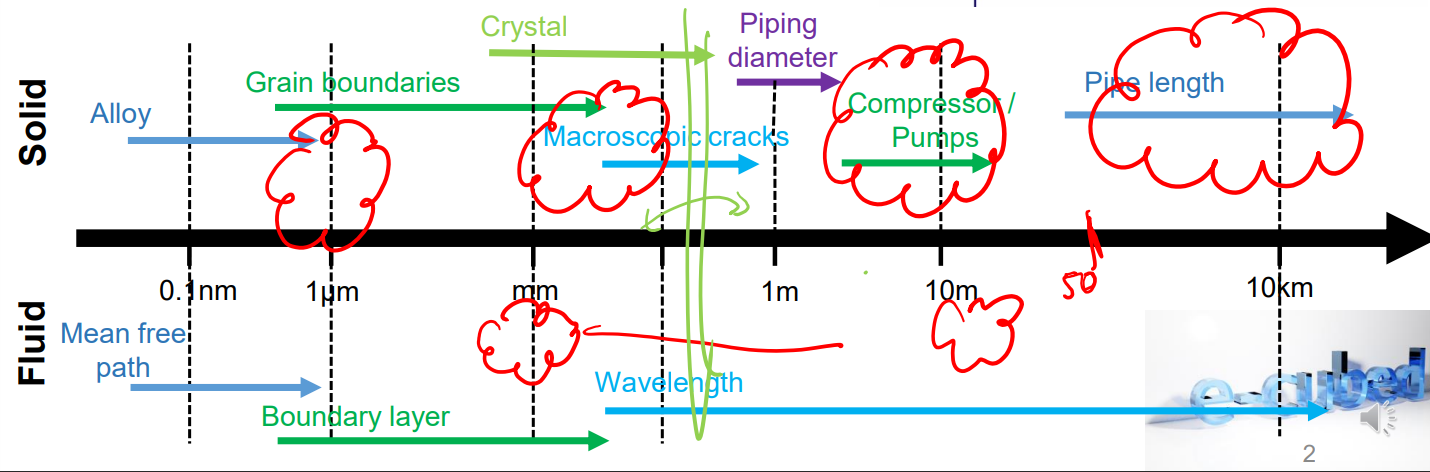
\includegraphics[width = \textwidth]{./img/figure1.png}
	\caption{Pressure pulsation in a piping system}
\end{figure}
\subsubsection{Cascade of length scales}
\begin{table}
	\begin{adjustbox}{width=\columnwidth,center}
		\begin{tabular}{@{}lll@{}}
			\toprule
			\textbf{Molecular}              & \textbf{Continuum}                            & \textbf{Structural}                     \\
			\midrule
			Material is made on this level  & Cracks operate on this level                  & Structures considered at this level     \\
			$< \SI{10}{\micro\meter}$       & $\SI{10}{\micro\meter} < x < \SI{10}{\meter}$ & $> \SI{10}{\meter}$                     \\
			Short range interactions        & Long range interactions                       & Whole scale interactions                \\
			Failure / corrosion / chemistry & Tune model - variables change                 & Long distance interaction               \\
			                                & continuously / smoothly (can account          & - vibration (waves transporting energy) \\
			                                & for discontinuous behaviour, e.g. crack)      &                                         \\
			\bottomrule
		\end{tabular}
	\end{adjustbox}
	\caption{Cascade of length scales}
\end{table}
\subsection{Complexity of the problem at different length scales}
Complexity of representation changes with the scale.
\begin{figure}[H]
	\centering
	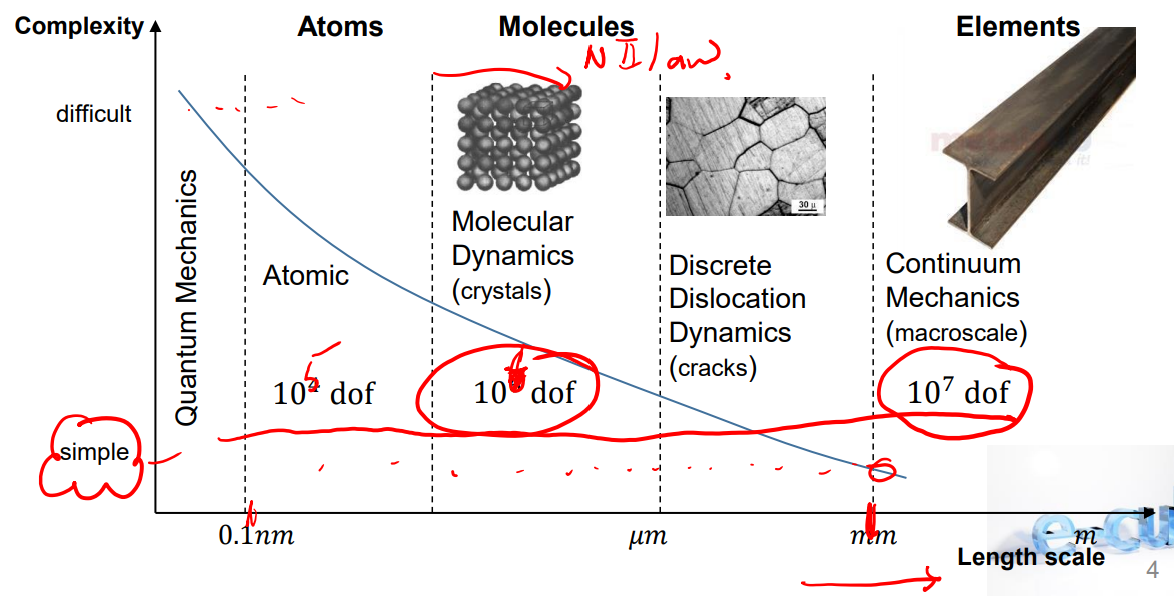
\includegraphics[width = \textwidth]{./img/figure2.png}
	\caption{Graph to show complexity against scale.}
\end{figure}
\subsection{Why focus on small scales?}
\begin{itemize}
	\item Small scale defects lead to crack initiation and propagation under external loading
	\item Failure can be corrected by changing material properties, for example, toughness
	\item Source of defects: complex chemical process (chemistry / corrosion) leads to corrosion at the surface
	\item Macroscale process is linked to microscale action
	\item Hypersonic flow - ionisation is non-continuum effect
	\item Analogy between defective liquids / solids
\end{itemize}
Note: turbulence is controlled by small vortices.
\subsubsection{Micrograph}
\begin{table}
	\centering
	\begin{tabular}{@{}ll@{}}
		\toprule
		\textbf{Domain}   & \textbf{Process}           \\
		\midrule
		Bulk              & Plasticity                 \\
		Internal boundary & Hydrogen embrittlement -   \\
		                  & plastic deformation / slip \\
		External boundary & Corrosion - chemistry      \\
		\bottomrule
	\end{tabular}
	\caption{Micrograph}
\end{table}
\begin{figure}[H]
	\centering
	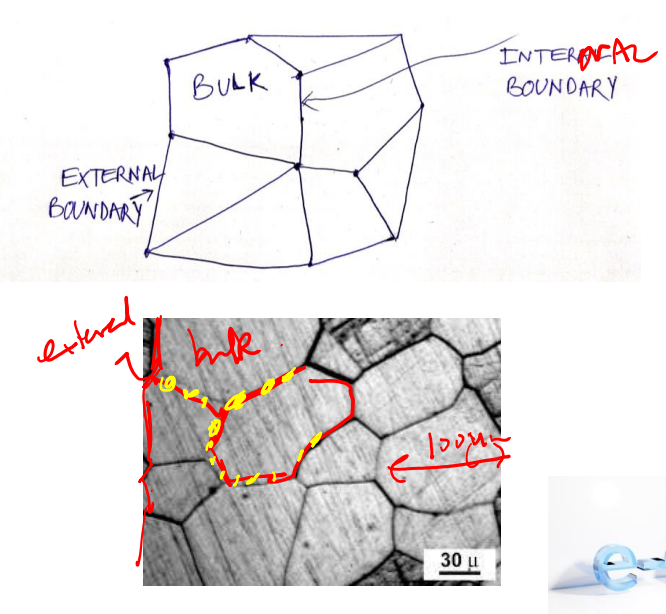
\includegraphics[width = 0.5\textwidth]{./img/figure3.png}
	\caption{Graph to show complexity against scale.}
\end{figure}
\subsubsection{Internal grain processes}
\begin{figure}[H]
	\centering
	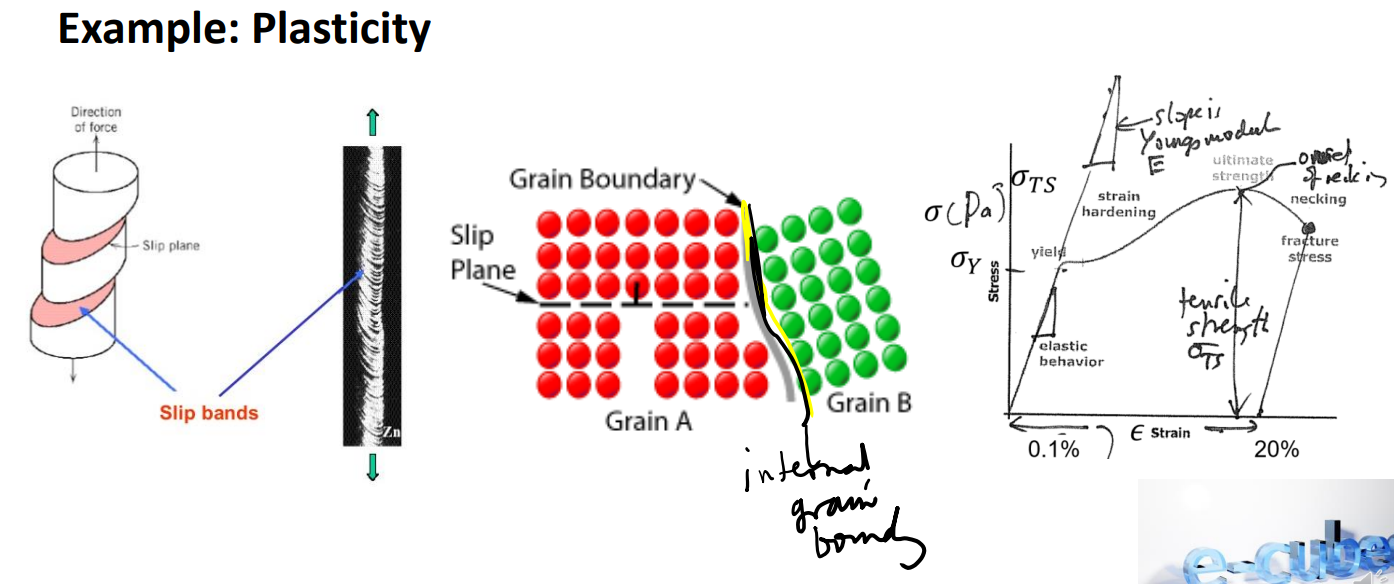
\includegraphics[width = 0.5\textwidth]{./img/figure4.png}
	\caption{Example of plasticity from internal grain process level.}
\end{figure}
\subsubsection{Internal boundary (hydrogen embrittlement - plastic deformation / slip)}
\begin{figure}[H]
	\centering
	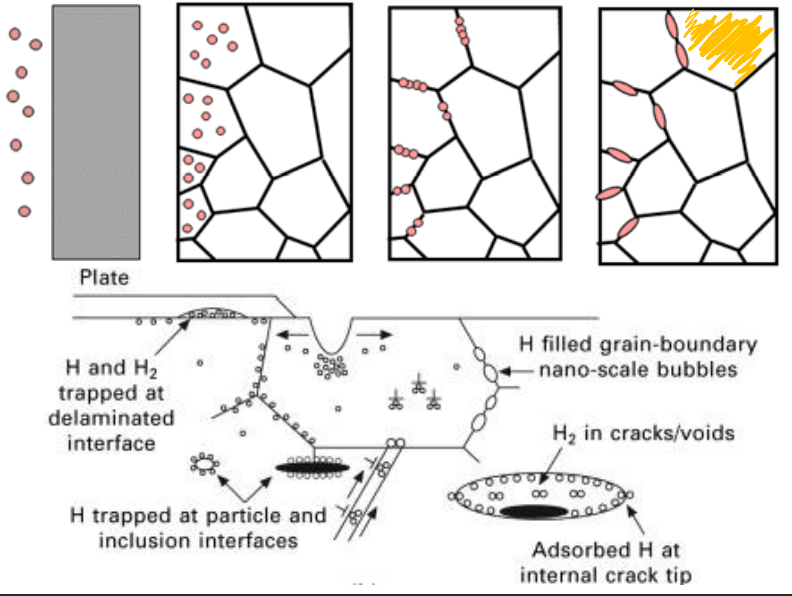
\includegraphics[width = 0.5\textwidth]{./img/figure5.png}
	\caption{Hydrogen embrittlement - plastic deformation / slip}
\end{figure}
\subsubsection{External boundary (corrosion)}
Corrosion happens over a long time and a range of scales. We need to understand how ions move around and interact with materials.
\begin{gather}
	\ce{Fe2 + (ag) + 2OH(ag) -> Fe(OH)_{2(s)}}\\
	\ce{4Fe(OH)_{2(s)} + O_{2(g)} + 2H2O_{(l)} -> Fe(OH)_{3(s)}}
\end{gather}
\begin{figure}[H]
	\centering
	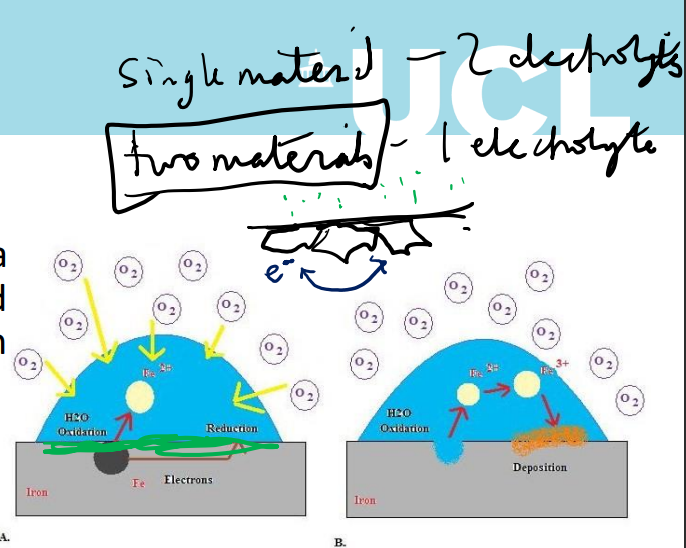
\includegraphics[width = 0.5\textwidth]{./img/figure6.png}
	\caption{Rust corrosion from grain boundary level.}
\end{figure}
\section{Categorisation of matter}
\begin{table}
	\centering
	\begin{tabular}{@{}lll@{}}
		\toprule
		\textbf{Matter} & \textbf{Modelling approach} &           \\
		\midrule
		Solid           & Atomistic                   & Continuum \\
		Gas             & Kinetic theory              & Continuum \\
		Liquid          & Molecular                   & Continuum \\
		\bottomrule
	\end{tabular}
	\caption{Categorisation of matter}
\end{table}
Switch between states are due to $p$, $V$ and $T$ and is represented by phase diagram. States of matter have been part of most religious and scientific texts for the last two thousand years, with water (aqua), fire (ignis), air (aer) and earth (terra) with the fifth being the void.
\section{Atomistic view of matter}
Typical length scale:
\begin{itemize}
	\item Diameter of atom is \SI{0.1}{\nano\meter} = \SI{1e-10}{\meter} = \SI{1}{angstrom}
	\item Nucleus diameter is \SI{1e-15}{\meter} (hydrogen) to \SI{15e-15}{\meter} (uranium-238)
\end{itemize}
\subsection{Bulk characteristic of materials}
The aim is to understand the relationship between the macrostructure and the microstructure. Key measures are:
\begin{itemize}
	\item Young's modulus $E = \left. \frac{\dif \sigma}{\dif \varepsilon} \right|_{\varepsilon \rightarrow 0}$
	\item Tensile stress: $\sigma_{TS}$
	\item Yields stress: $\sigma_{Y}$
	\item Ductility: $\epsilon_{T}$
\end{itemize}
It is important to understand the following:
\begin{table}
	\centering
	\begin{tabular}{@{}lll@{}}
		\toprule
		\textbf{Properties} &                                   & \textbf{Definition}                                \\
		\midrule
		Elastic modulus     & $E$ (\si{\pascal})                & Measure of material resistance to deformation.     \\
		Yield stress        & $\sigma_Y$ (\si{\pascal})         & Measure of stress at which the elastic behaviour   \\
		                    &                                   & disappears and plastic behaviour initiates.        \\
		Hardness            & HBW                               & Measure of material resistance to indentation      \\
		Creep               &                                   & Time-dependant deformation at high temperature     \\
		                    &                                   & and constant stress.                               \\
		Toughness           & $K$ (\si{\joule\per\meter\cubed}) & Resistance to crack propagation.                   \\
		Ductility           & $\epsilon_T$                      & Material's ability to undergo plastic deformation. \\
		\bottomrule
	\end{tabular}
	\caption{Key points on material properties}
\end{table}
How are they related to the microstructure?
\subsection{Newtonian model of matter}
Useful for biological, physical problems, solids, liquids and gases. This is based on a description of matter as a collection of point particles, an approach that is useful for gases, liquid and solids. The dynamics of the i-th molecule is:
\begin{gather}
	\underline{F}_i = \sum_{j,j} \neq \nabla U\left(x_i,x_j\right)
\end{gather}
Located at point $\underline{x}_i$ whose dynamics are:
\begin{gather}
	m_i \dfrac{\dif \underline{v}_i}{\dif t} = \underline{F}_i\\
	\underline{v}_i = \frac{\dif \underline{x}_i}{\dif t}
\end{gather}
The formulation requires the form of the interaction stated using the Lennard-Jones 6-12 potential:
\begin{gather}
	U = 4 \epsilon \left(\left(\frac{\sigma}{r}\right)^{12} - \left(\frac{\sigma}{r}\right)^6\right) + \dots
\end{gather}
The difficultly is that neighbourhood lists are kept and only sum over local interaction of molecules.
\begin{itemize}
	\item Not hard collision
	\item Time stepping fixed
	\item Potentials can be empirical or chosen to now slow down calculations
\end{itemize}
\begin{gather}
	U = U_{stretch} + U_{bend} + U_{torsion} + U_{vanderWaal} + U_{electro} + U_{cross}
\end{gather}
Research gaps:
\begin{itemize}
	\item Link between continuum and molecular
	\item Quantum - mechanical models
\end{itemize}
\subsection{Vibrational modes and energy}
Mechanical representation of matter. Molecules interact with their neighbours and fields. Interaction may be quite far, particularly when charges are important. We are familiar with how degrees of freedom influence properties of a gas, especially through the isentropic index. Energy is stored in various modes of vibration e.g. gas. This is called classical molecular dynamics.
\subsection{Molecular description of material properties}
\subsubsection{Primary bonds}
Ionic and covalent bonds are extremes with most (electron distribution) bonds lying between (polar covalent)
\begin{figure}[H]
	\centering
	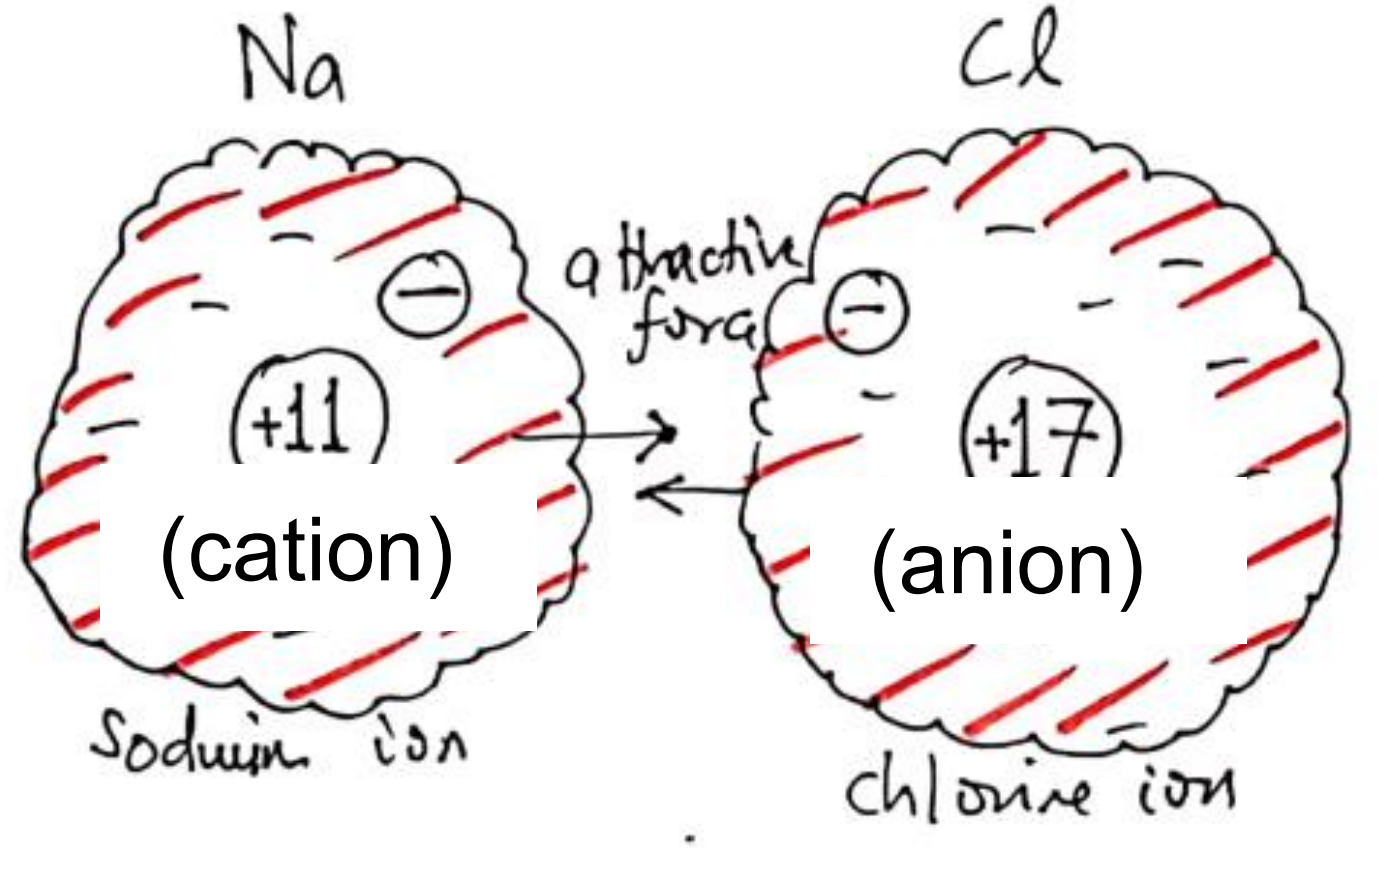
\includegraphics[width = 0.5\textwidth]{./img/figure7.png}
	\caption{Ionic bond (electrovalence)}
\end{figure}
\begin{gather}
	F = \frac{q_1 q_2}{4\pi \epsilon_0 r^2}\\
	U = U_i - \frac{q^2}{4\pi\epsilon_0 r} + \frac{B}{r^n}
\end{gather}
\begin{figure}[H]
	\centering
	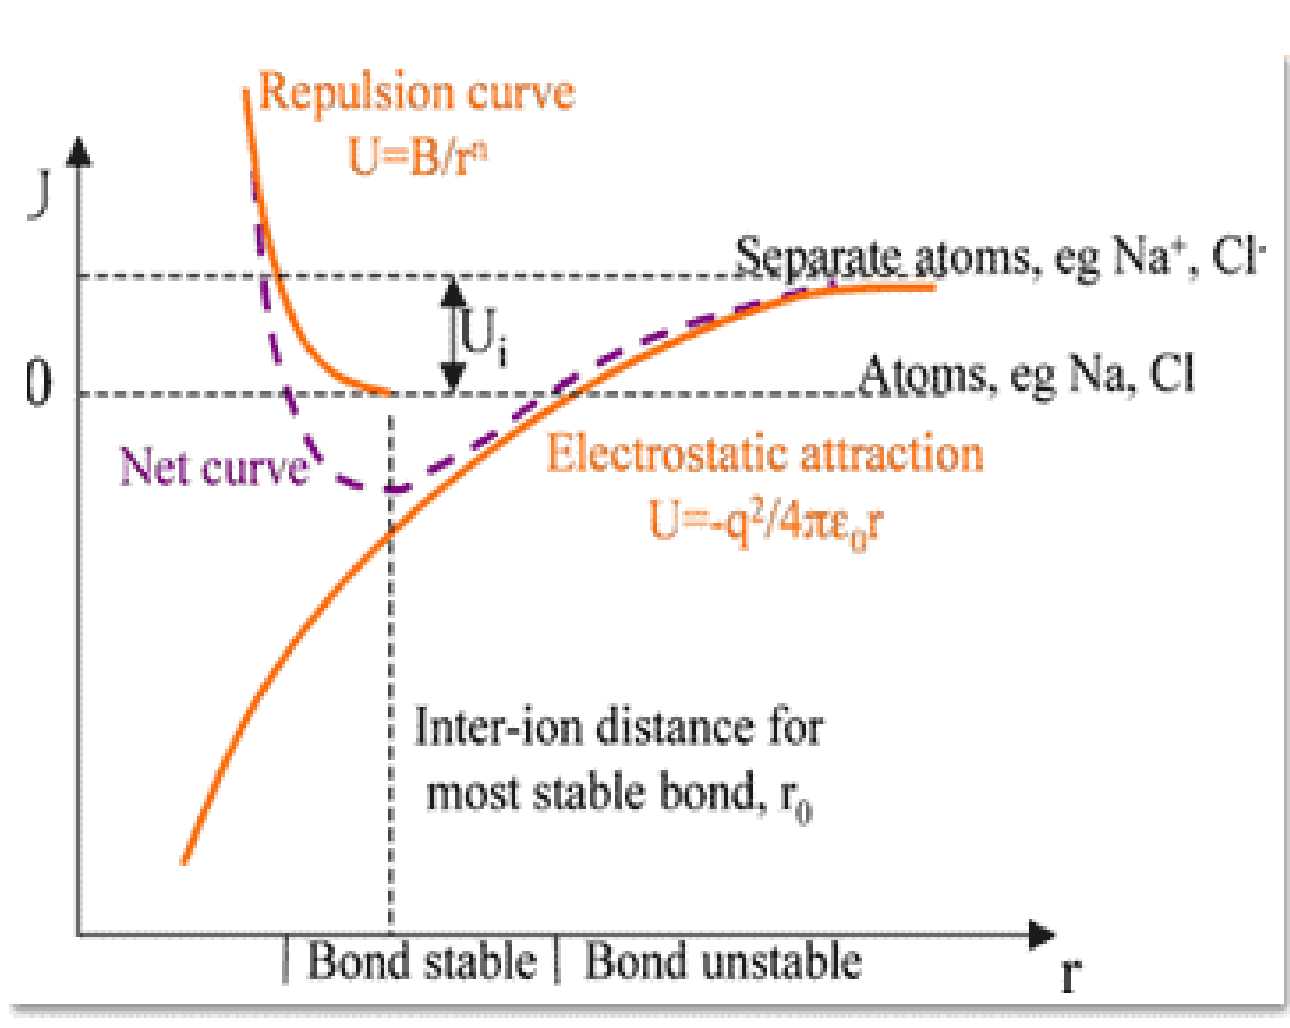
\includegraphics[width = 0.5\textwidth]{./img/figure8.png}
	\caption{Bond stability.}
\end{figure}
\begin{figure}[H]
	\centering
	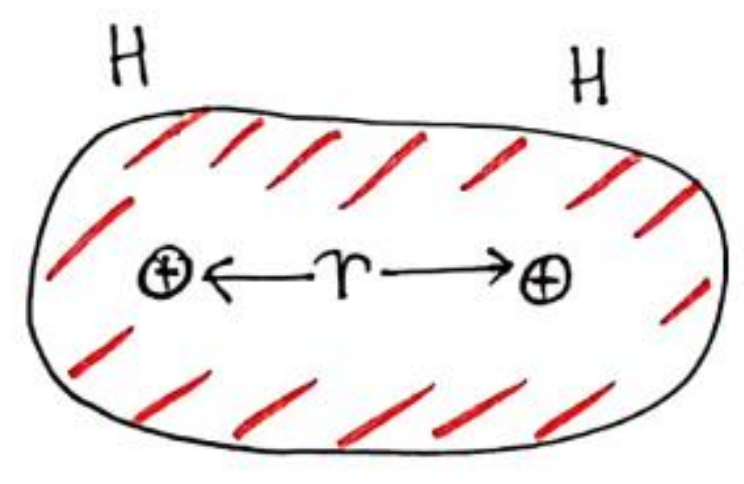
\includegraphics[width = 0.5\textwidth]{./img/figure9.png}
	\caption{Covalent bond (covalence). Note the overlap of electron orbit.}
\end{figure}
\begin{gather}
	U = -\frac{A}{r^m} + \frac{B}{r^n}, \, m<n
\end{gather}
\begin{figure}[H]
	\centering
	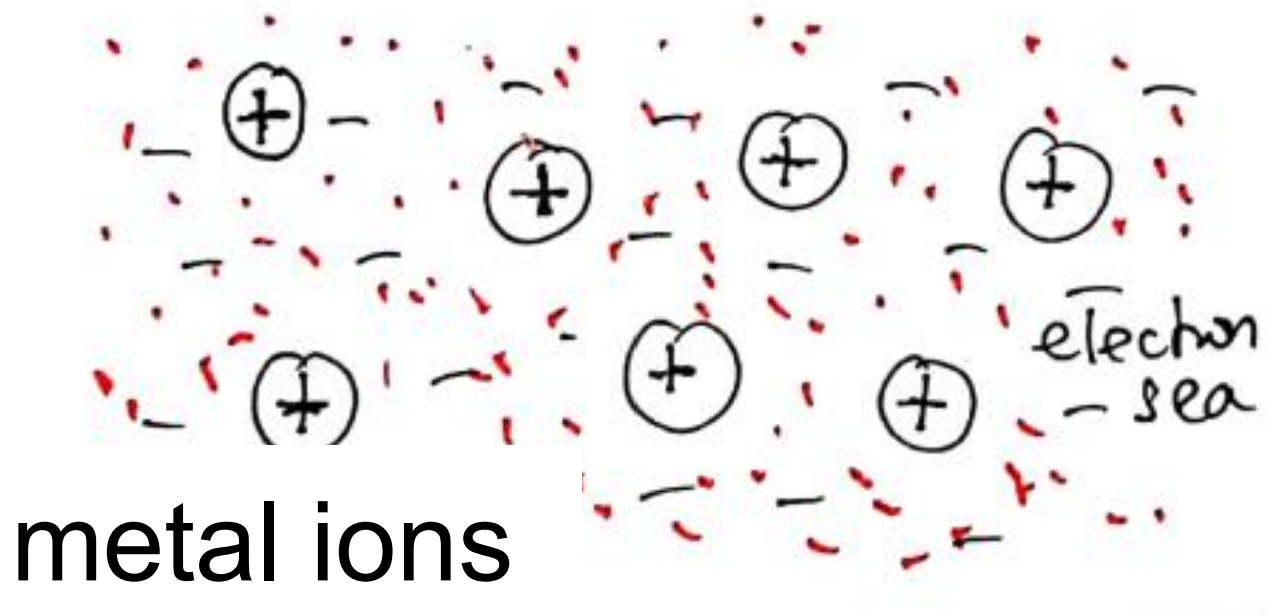
\includegraphics[width = 0.5\textwidth]{./img/figure10.png}
	\caption{Metallic bond (electron cloud).}
\end{figure}
\begin{gather}
	e = \SI{1.6e-19}{C}\\
	\epsilon_0 = \SI{8.8e-12}{Nm^2C^{-2}}\\
	\SI{1}{eV} = \SI{1.6e-19}{J}
\end{gather}
\subsubsection{Secondary bonds}
The secondary bonds are important - without them many gases would not condense. The relative displacement of the positive and negative charge gives rise to a dipolar force. This gives rise to an attractive force. Most usual form is the Lennard Jones 6-12 potential.
\begin{gather}
	U = -\frac{A}{r^6} + \frac{B}{r^n}
\end{gather}
\begin{figure}[H]
	\centering
	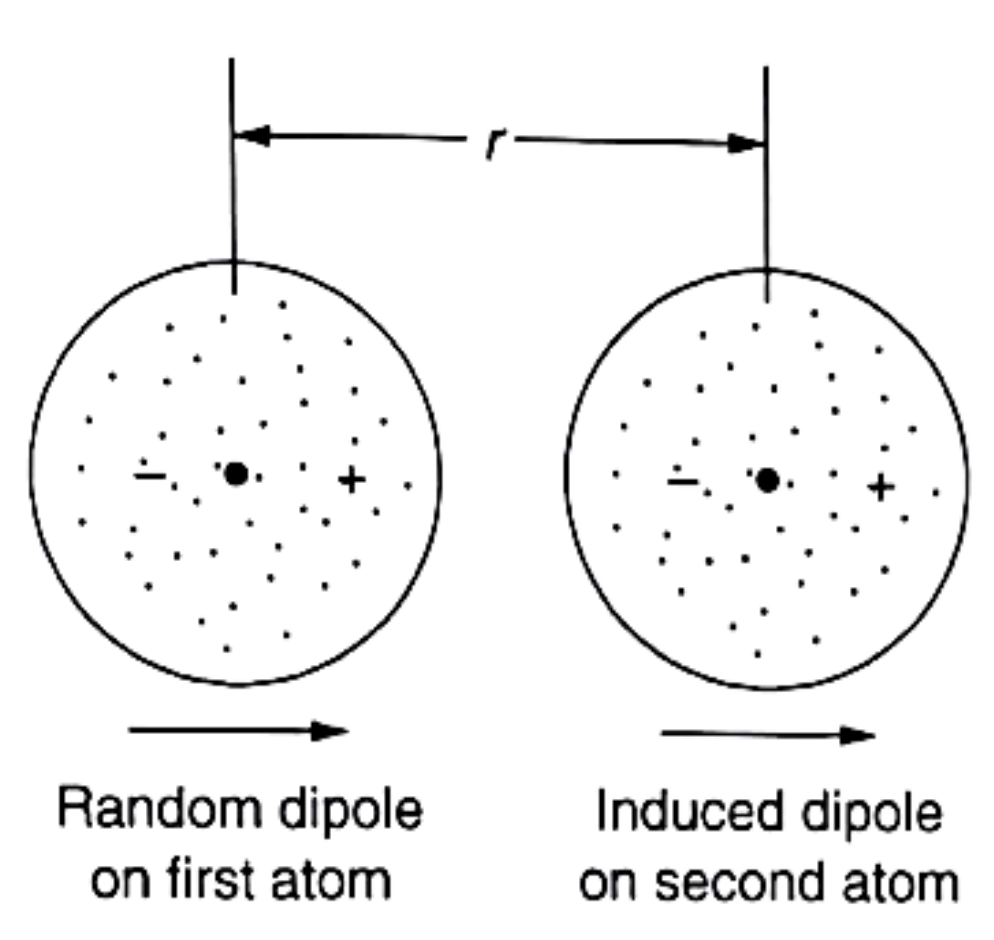
\includegraphics[width = 0.5\textwidth]{./img/figure11.png}
	\caption{Secondary bonds. Note: long range attractive force -  dipole-dipole interactions. Overlapping electron orbits - repulsive.}
\end{figure}
\subsubsection{Physical basis of Young's Modulus}
Classical mechanics:
\begin{gather}
	m\frac{\dif v}{\dif t} = \frac{\dif U }{\dif r}
\end{gather}
where $U$ is the potential energy. At equilibrium:
\begin{gather}
	\frac{\dif U}{\dif r } = 0
\end{gather}
so that close to this point, the energy potential can be expanded to give:
\begin{gather}
	m \frac{\dif^2 r }{\dif t^2} = \left(\frac{\dif^2 U}{\dif r^2}\right)\left(r-r_0\right)
\end{gather}
Around equilibrium point:
\begin{gather}
	F = S_0 \left(r - r_0\right)\\
	S_0 = -\frac{\dif^2 U}{\dif r^2}
\end{gather}
The stress is:
\begin{gather}
	\sigma = N S_0 \left(r - r_0\right) = \frac{S_0\left(r-r_0\right)}{r_0^2}
\end{gather}
The Young's modulus is:
\begin{gather}
	E = \frac{\sigma}{\epsilon} = \frac{S_0}{r_0}
\end{gather}
Estimate:
\begin{gather}
	S_0 = \frac{\alpha q^2}{4\pi\epsilon_0r^2}\\
	E = \frac{\sigma}{\epsilon} = - \frac{\frac{\dif^2 U}{\dif r^2}}{r_0} = \frac{\delta e^2}{4\pi\epsilon_0r_0^4}
\end{gather}
Atom spacing:
\begin{gather}
	\overline{r}_0 \approx 8.54
\end{gather}
\begin{figure}[H]
	\centering
	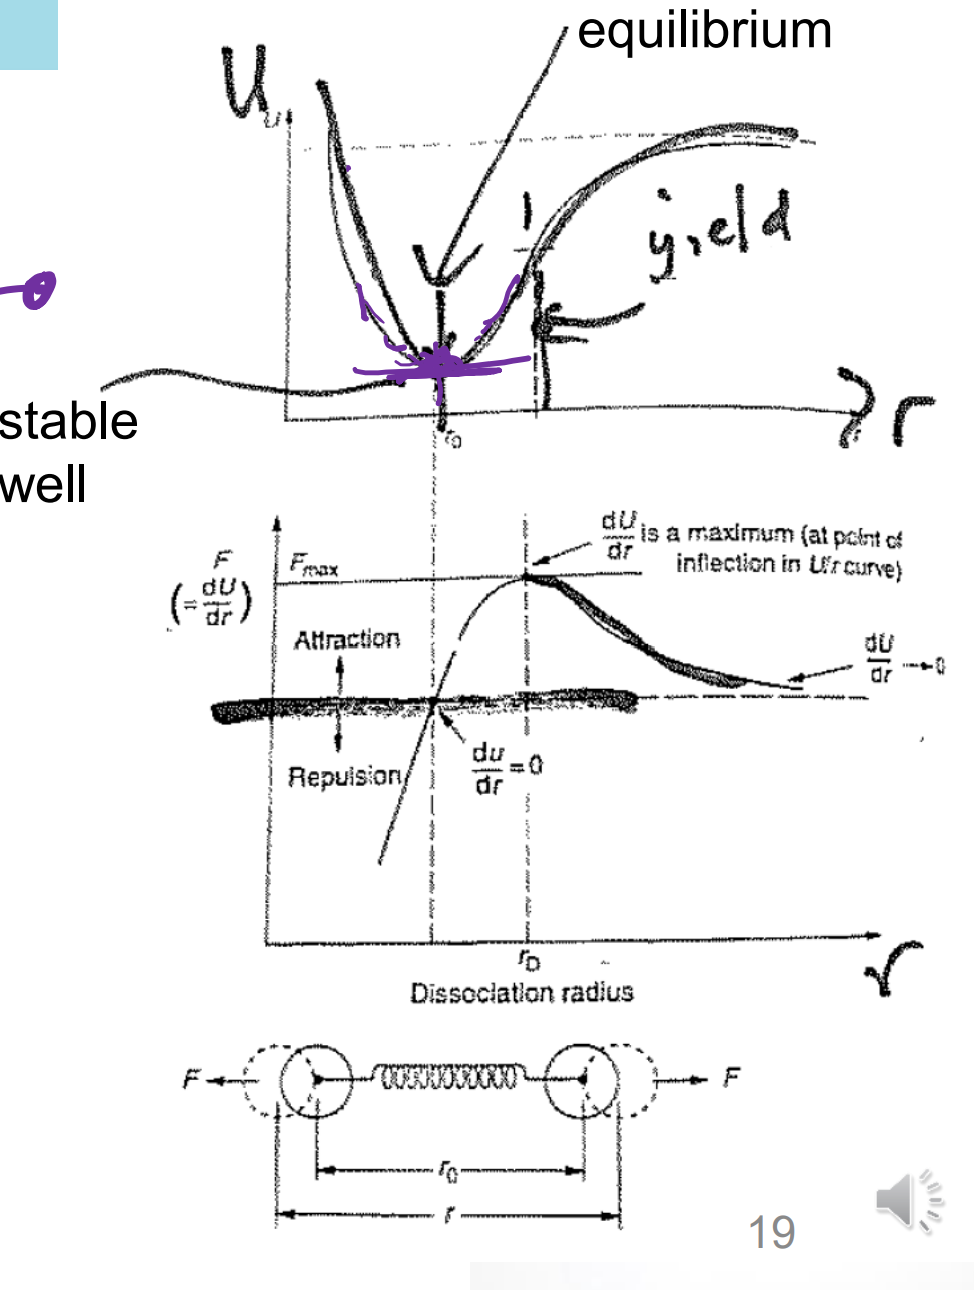
\includegraphics[width = 0.5\textwidth]{./img/figure12.png}
	\caption{Young's modulus from atomic perspective.}
\end{figure}
\subsubsection{Comparison between molecular and macroscopic measurements}
\begin{table}[H]
	\centering
	\begin{tabular}{@{}llll@{}}
		\toprule
		\textbf{Bond type} & $S_0$ / \si{Nm^{-1}} & \textbf{Young's modulus estimate} & \textbf{Measurement}       \\
		                   &                      & $E$ / \si{\giga\pascal}           &                            \\
		\midrule
		Covalent           & 50 - 180             & 200 - 1000                        & 1000 (diamond)             \\
		Metallic           & 15 - 75              & 60 - 300                          & 200 (nickel)               \\
		Ionic              & 8 - 24               & 32 - 96                           & 15 - 91 (alkali halides)   \\
		H-Bond             & 2 - 3                & 8 - 12                            & 9.1 (ice)                  \\
		van der Waals      & 0.5 - 1              & 2 - 4                             & 0.01 - 2 (rubber to nylon)
	\end{tabular}
	\caption{Comparison between molecular and macroscopic measurements.}
\end{table}
\subsubsection{Estimation of yield stress}
Returning to the molecular model since:
\begin{gather}
	U = \epsilon \left(-\frac{A}{r^6} + \frac{B}{r^{12}}\right)\\
	U'' = \epsilon \left(- \frac{6\times 7A}{r^8} + \frac{12\times 13B}{r^{14}}\right)
\end{gather}
Then, maximum stress is:
\begin{gather}
	\sigma_Y \approx \frac{E}{8}
\end{gather}
Therefore:
\begin{gather}
	\frac{\sigma_Y}{E} ~ \frac{1}{8}
\end{gather}
This estimated ratio is good for ceramics, but not good for metals. So what is missing from a molecular description?
\begin{figure}[H]
	\centering
	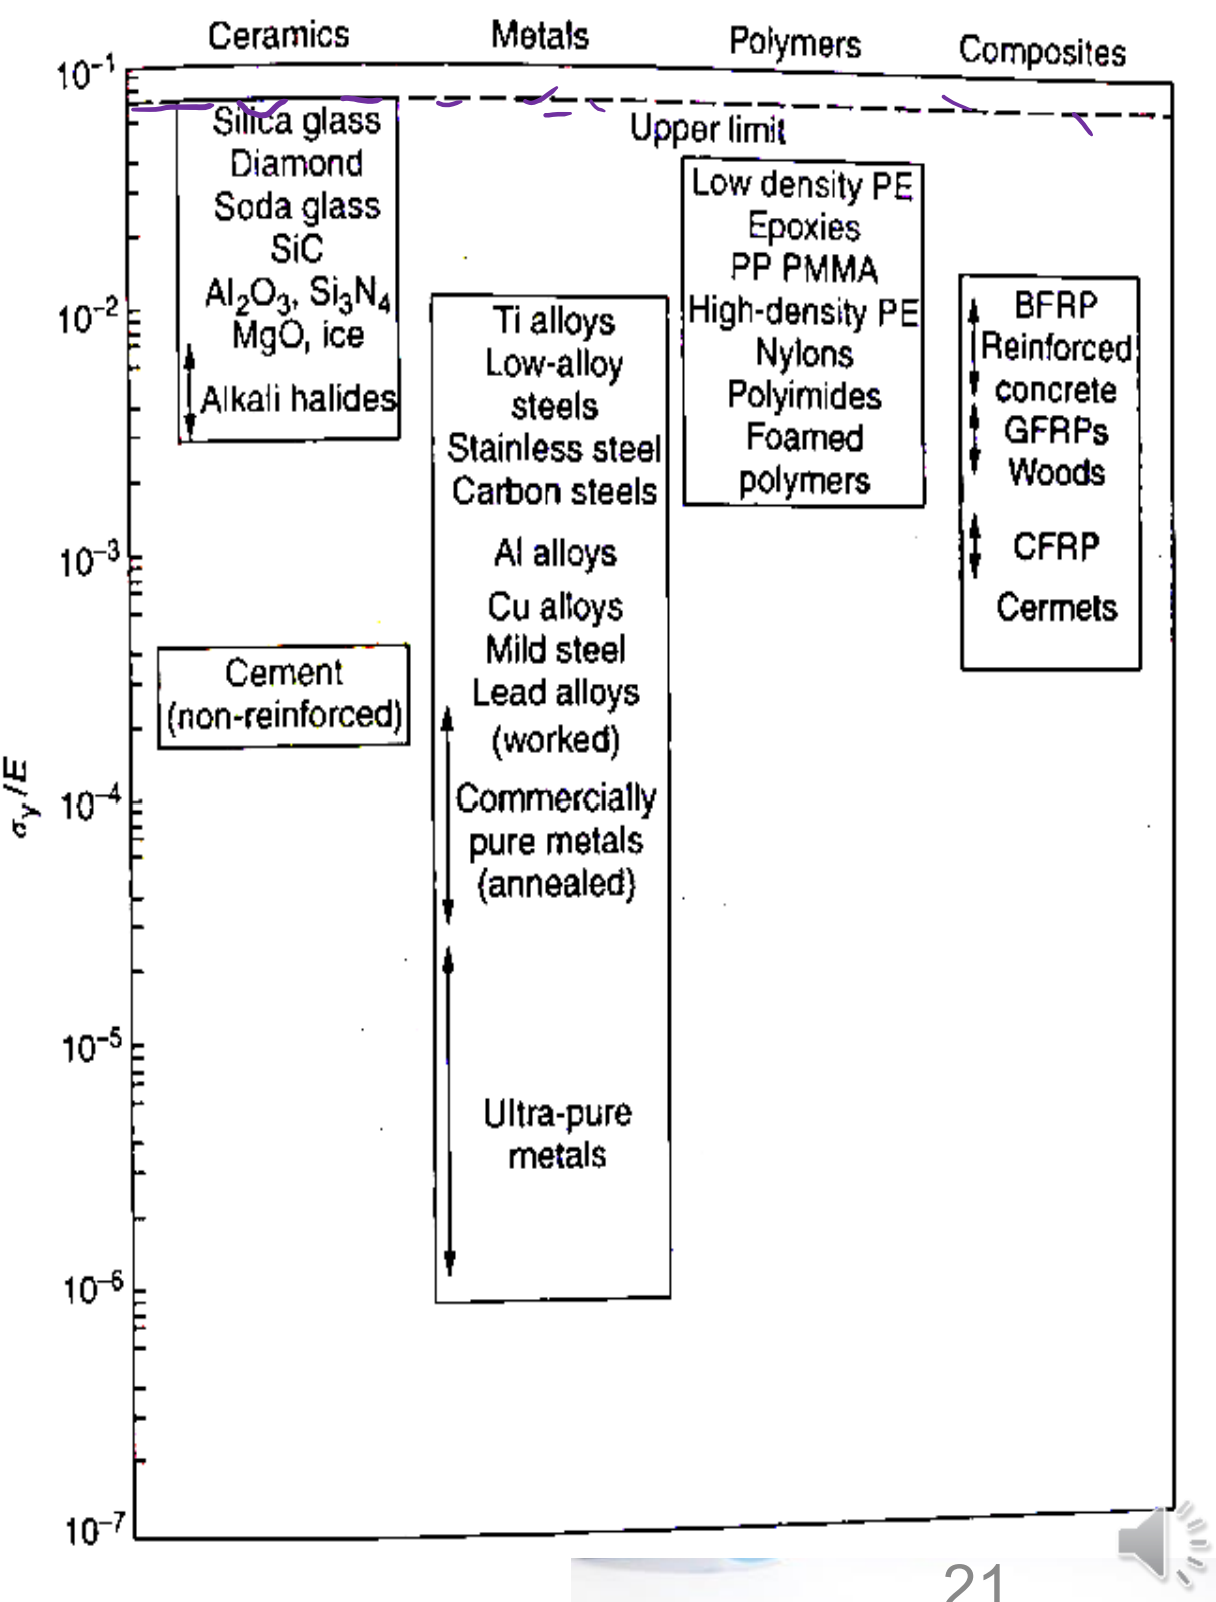
\includegraphics[width = 0.5\textwidth]{./img/figure13.png}
	\caption{Graph to show yield stress ratio for different materials.}
\end{figure}
\subsection{Material classification}
\begin{itemize}
	\item Metals
	      \begin{itemize}
		      \item Ferrous metals and alloys
		      \item Non ferrous metals and alloys
		      \item (focus on here)
	      \end{itemize}
	\item Polymeric (non metallic, non crystalline)
	      \begin{itemize}
		      \item Thermoplastic plastics
		      \item Thermoset plastics
		      \item Elastomers
	      \end{itemize}
	\item Ceramics
	      \begin{itemize}
		      \item Glass
		      \item Diamond
		      \item Glass ceramics
	      \end{itemize}
	\item Composites (everything else)
	      \begin{itemize}
		      \item Metal-matrix composites
		      \item Sandwich structures
		      \item Concrete
	      \end{itemize}
\end{itemize}
\subsubsection{Three common configurations}
\begin{table}[H]
	\centering
	\begin{tabular}{@{}llll@{}}
		\toprule
		\textbf{Type} & \textbf{Name}               & \textbf{Description}      & \textbf{Example}             \\
		\midrule
		BCC           & Body centred cube - 2 atoms & Harder and less malleable & Lithium, Sodium, Potassium   \\
		              &                             & Packing factor 0.68       & Chromium, Barium, Alpha-iron \\
		FCC           & Face centred cube           & malleable, softer 0.74    & Copper, Gold, Aluminium      \\
		              &                             &                           & Iridium, Lead, Nickel, etc.  \\
		HCP           & Hexagonal close packed      & 6 atoms                   & Cadmium, Magnesium, Titanium \\
		              &                             & Packing ratio 0.74        & Zinc, Zirconium              \\
		\bottomrule
	\end{tabular}
	\caption{Configurations of atoms.}
\end{table}
\subsubsection{Solidification and crystal growth}
Under normal circumstances, crystal growth starts at many nucleation points. Solidification leads to crystals growing and stop growing when they meet another crystal. A crystal is usually called a grain. The boundary between grains is the grain boundary where structure is disordered. This is controlled using nucleation points and directional solidification and liquid freezing-dendritic growth and shrinkage occurs during cooling.
\begin{figure}[H]
	\centering
	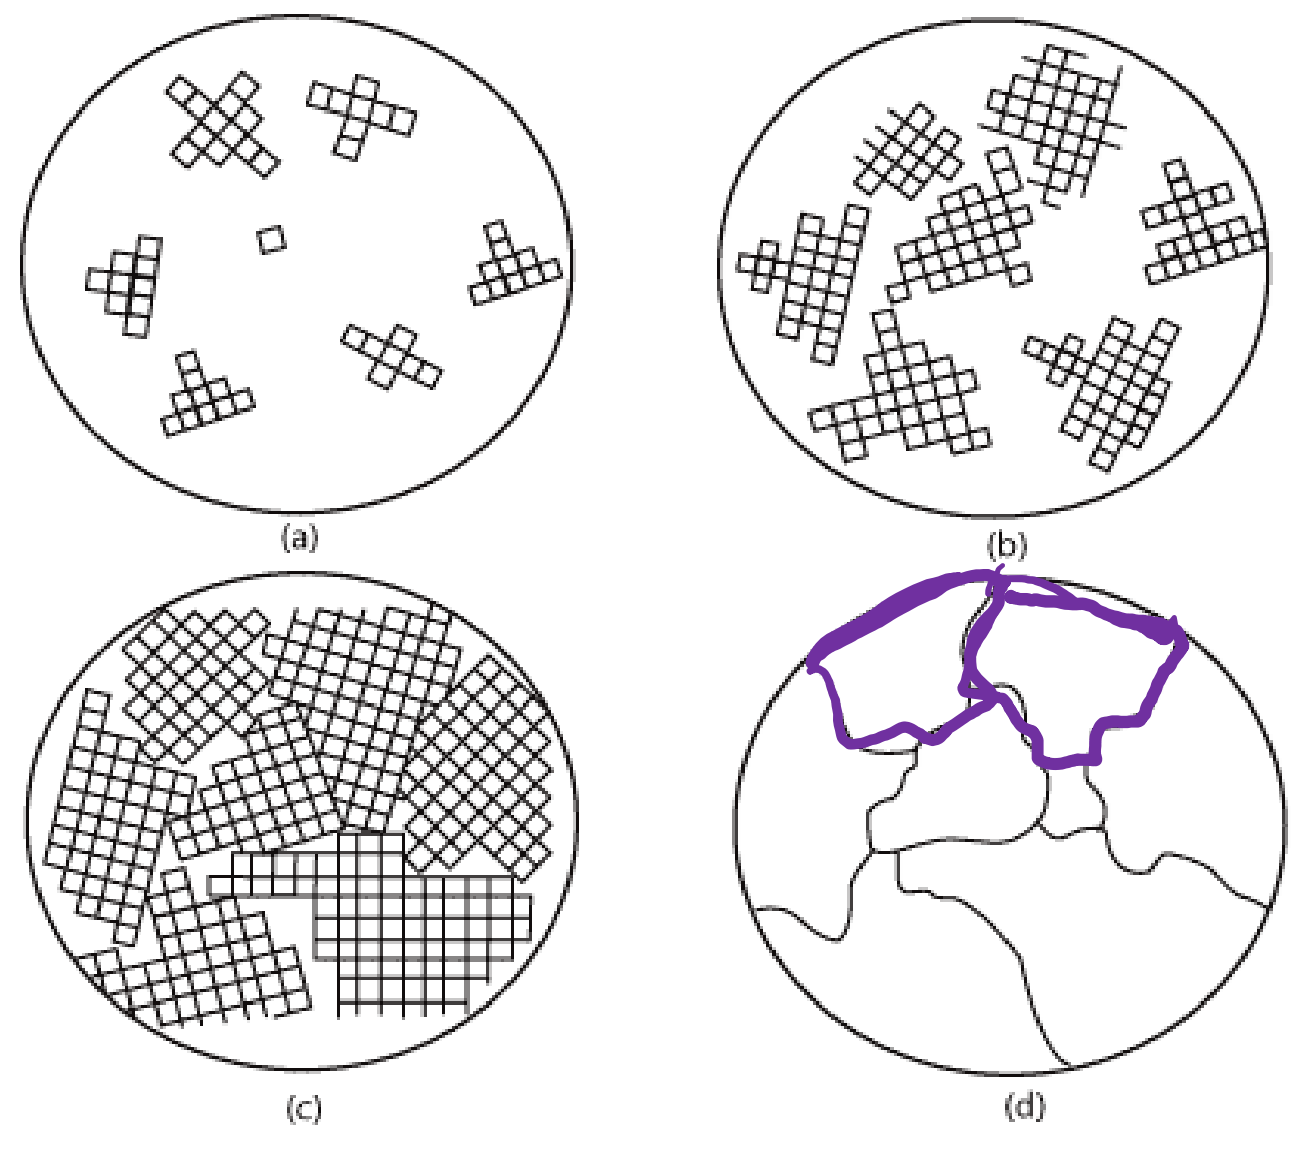
\includegraphics[width = 0.6\textwidth]{./img/figure14.png}
	\caption{Nucleation of crystals.}
\end{figure}
\subsubsection{Crystal defects}
Three types of defects:
\begin{enumerate}
	\item Point defects: which are places where an atom is missing or irregularly placed in the lattice structure. Point defects include lattice vacancies, self interstitial atoms, substitution impurity atoms and interstitial impurity atoms
	\item Linear defects: which are groups of atoms in irregular positions. Linear defects are commonly called dislocations
	\item Planar defects: which are interfaces between homogeneous regions of the material. Planar defects include grain boundaries, stacking faults and external surfaces
\end{enumerate}
\subsubsection{Atomistic view of plastic deformation}
Elastic deformation - stress is small, the metal can recover to initial state when the stress is removed. This involves stretching the bonds but atoms do not mover over one another.

Plastic deformation - stress is large, plastic deformation involves the breaking of a limited number of atomic bonds by the movement of dislocations. Since the energy required to move is lowest along the densest planes of atoms, dislocations have a preferred direction of travel within a grain of the material. This results in slip that occurs along parallel planes within the grain. These parallel slip planes group together to form slip bands. A slip band appears as a single line under the microscope, but it is in fact made up of closely spaced parallel slip planes as shown in the image.
\begin{figure}[H]
	\centering
	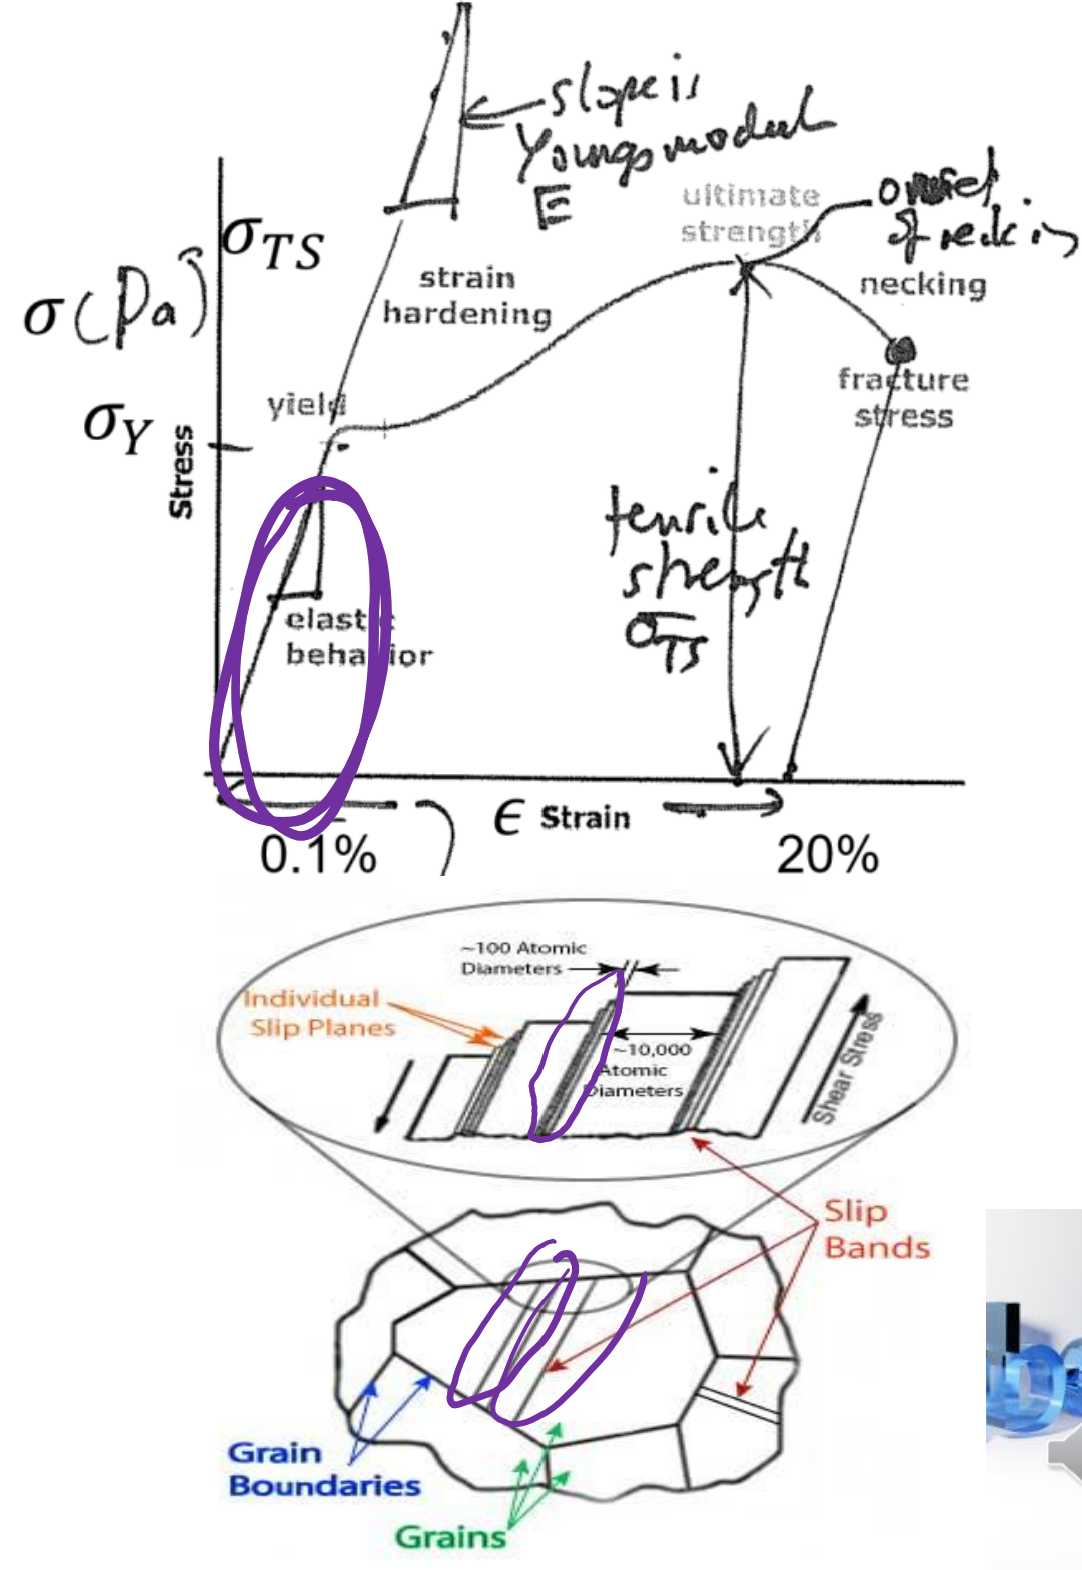
\includegraphics[width = 0.5\textwidth]{./img/figure15.png}
	\caption{Stress-strain curve.}
\end{figure}
\subsubsection{Fatigue crack initiation}
The life of a fatigue crack has two parts, initiation and propagation. Dislocations play a major role in the fatigue crack initiation phase. It has been observed in laboratory testing that after a large number of loading cycles dislocation pule up and form structures called persistent slip bands. Initiation has a molecular origin.
\subsubsection{Topological change in crystal structure}
\begin{figure}[H]
	\centering
	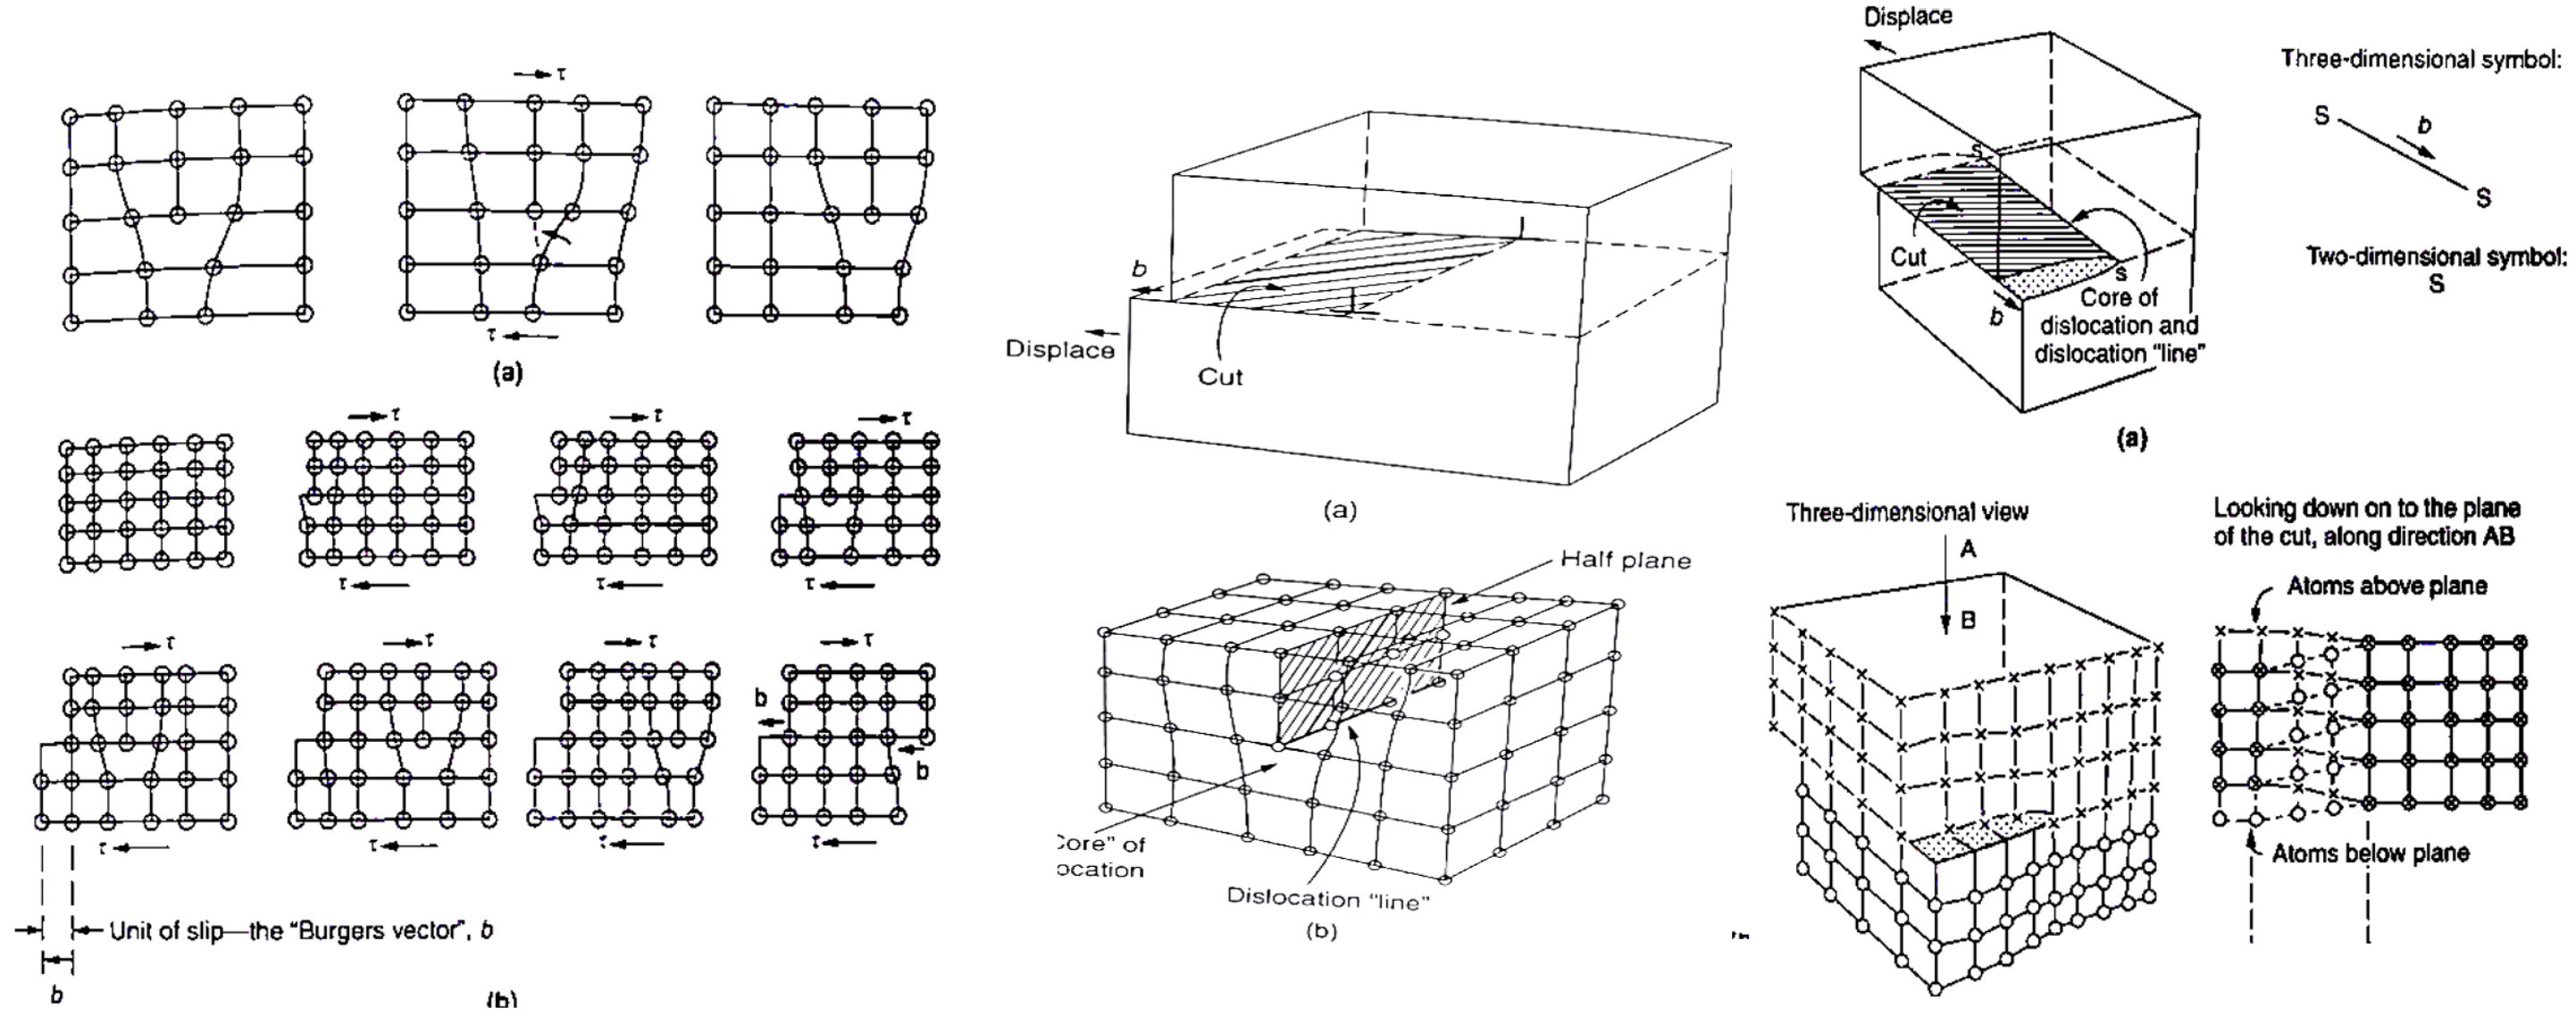
\includegraphics[width = 0.5\textwidth]{./img/figure16.png}
	\caption{Topological changes in crystal structure.}
\end{figure}
\section{Kinetic theory of gases}
Statistical 19th century view of macroscopic properties of gas. Boltzmann and colleagues developed new techniques to describe matter. Heavily influenced the theory of turbulence $\leftarrow$ based on kinetic theory of a gas.

$p = \rho RT$ origin with statistical theory.

This is an excellent macroscopic model of matter. The problem is that it does not work well for low pressure, high pressure or when density is low (and continuum concepts don't work).
\subsection{Speed of molecules}
Results tell us about average speed but not the distribution.
\begin{gather}
	n_v\left(E\right) = n_0 e^{-\frac{E}{k_B T}}
\end{gather}
where, $n_v\left(E\right)$ is the Boltzmann distribution which coups a lot. The speed of the molecules satisfies the Maxwell-Boltzmann distribution.
\begin{gather}
	f\left(v\right) = 4\pi \left(\frac{m}{2\pi k_B T}\right)^3 v^2 \exp{\left(-\frac{mv^2}{2k_B T}\right)}
\end{gather}
\begin{figure}[H]
	\centering
	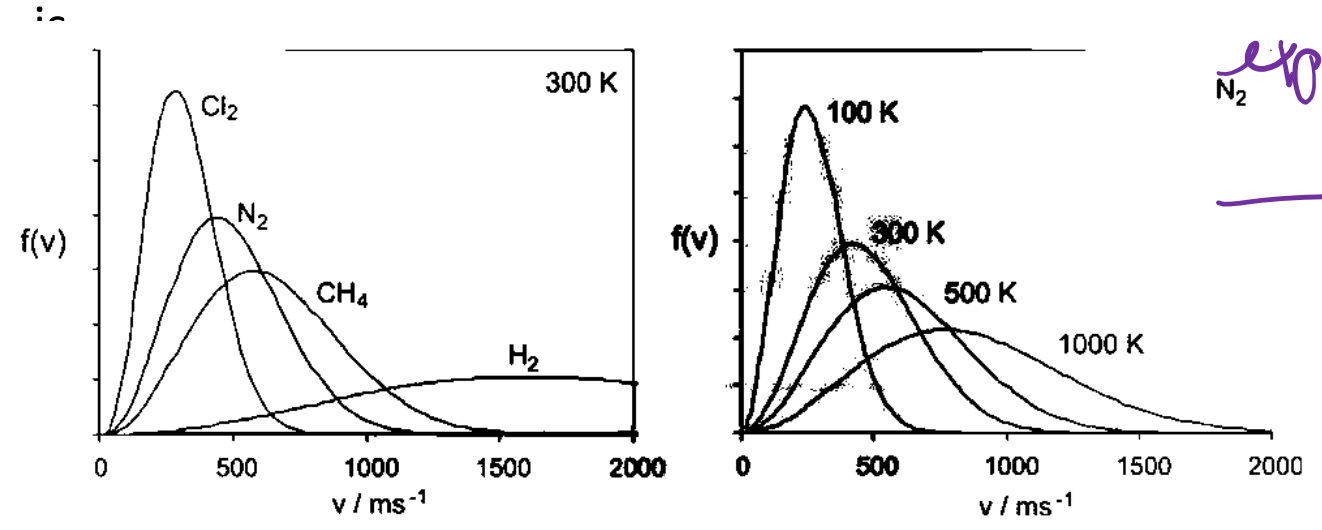
\includegraphics[width = 0.7\textwidth]{./img/figure17.png}
	\caption{Speed of molecules.}
\end{figure}
\subsection{Equations of state of real gases}
The molecular continuum view of matter are linked. Virial equation:
\begin{gather}
	pV = nRT\left(1 + \frac{B}{V_m} + \frac{C}{V_m^2} + \dots\right)
\end{gather}
where $B$, $C$ are the second and third virial coefficients. Van der Waals equation:
\begin{gather}
	\left(p + a\frac{n^2}{V^2}\right)\left(V - nb\right) = nRT \textrm{ or}\\
	P = \frac{nRT}{V- nb} - a \frac{n^2}{V^2}
\end{gather}
$n$ is the number of moles. $nb$ is the volume excluded since molecules cannot overlap. $\frac{an^2}{V^2}$ pressured reduced due to attractions between pairs of molecules.
\subsubsection{Critical constants for van der Waals equation}
Solving these two equations in two unknowns (temperature and molar volume) gives the critical temperature and critical molar volume:
\begin{gather}
	T_c = \frac{8a}{27Rb}\\
	V_c = 3b
\end{gather}
\subsubsection{Van der Waals}
\begin{figure}[H]
	\centering
	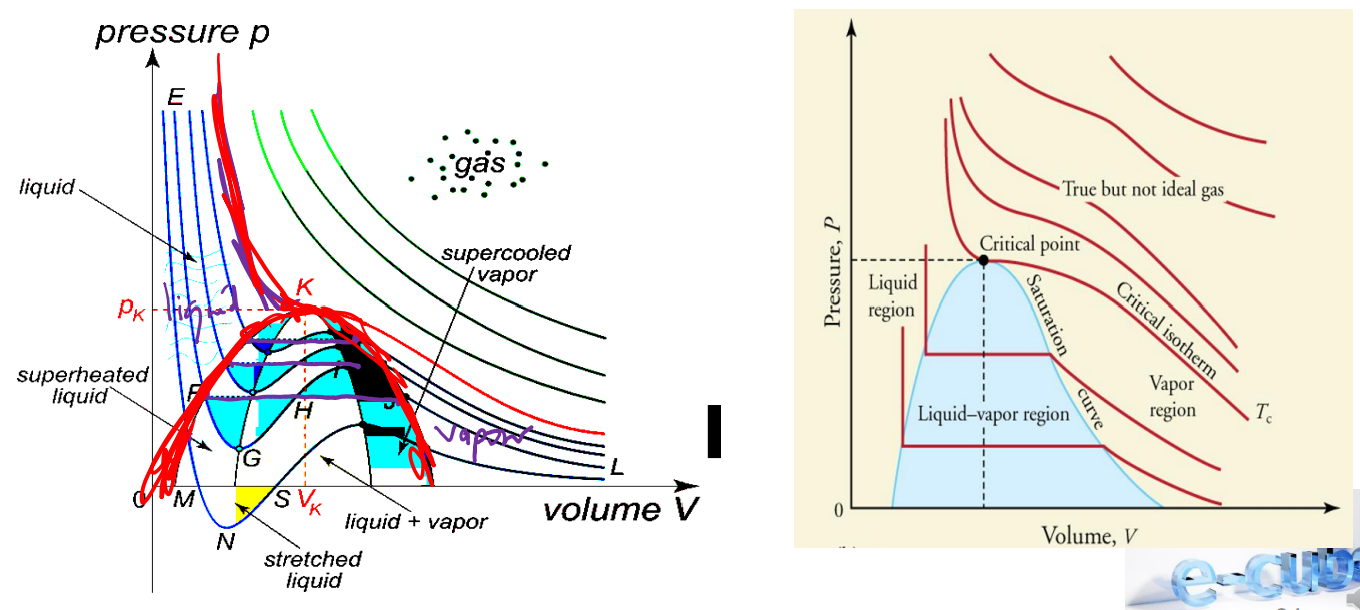
\includegraphics[width = 0.7\textwidth]{./img/figure18.png}
	\caption{Van der Waals.}
\end{figure}
\subsubsection{Link between molecular and microscopic}
Most of the important 19th century breakthroughs were determining link between macroscopic (could be seen) and microscopic (could not be seen). For example, Brownian motion:
\begin{gather}
	\frac{RT}{5\pi\mu dN_A} = D = \lim_{t\rightarrow \infty} \frac{\left(x^2\right)}{2t} \approx \SI{10e-10}{\meter\squared\per\second}
\end{gather}
This represented a link between Avogadro's constant and macroscopic movement of particles. Here $N_A = \SI{6e23}{\per\mole}$. Theory by Einstein (1905) and Sutherland (1905). Millikans experiments: determination of the charge on an electron. The link between molecular and microscopic last areas of modern science to be worked out.
\subsubsection{Einstein theory and Millikans experiment}
Based around kinetic theory of gases and momentum change due to collision. Pressure is a manifestation of a:
\begin{gather}
	P = \frac{2}{3}\frac{N}{V}\frac{1}{2}m_0 \overline{v}^2\\
	\therefore PV = nRT = \frac{N}{N_a}RT = Nk_BT\\
	\therefore KE = \frac{3}{2}Nk_bT = \frac{3}{2}nRT = \frac{NDF}{2}nRT
\end{gather}
where $NDF$ is number of degrees of freedom.
\subsubsection{Model assumptions}
\begin{itemize}
	\item No intermolecular forces between the gas particles
	\item The volume occupied by the particles is negligible compared to the volume of the container they occupy
	\item The only interactions between the particles and with the container walls are perfectly elastic collisions.
	\item Real gas, the atoms or molecules have a finite size, and at close range they interact with each other through a variety of intermolecular forces, including dipole-dipole interactions, dipole induced dipole interactions and van der Waal's (induced dipole - induced dipole) interactions
	\item When applied to real gases, the ideal gas model breaks down when molecular size effects or intermolecular forces become important. This occurs under conditions of high pressure , when the molecules are forced close together and therefore interact strongly, and at low temperatures, when the molecules are moving slowly and intermolecular forces have a long time to act during a collision
\end{itemize}
The pressure at which the ideal gas model starts to break down will depend on the nature and strength of the intermolecular forces between the gas particles, and therefore on their identity. The ideal gas model becomes more and more exact as the pressure is lowered, since at very low pressures the gas particles are widely spaced apart and interact very little with each other.
\begin{gather}
	\textrm{number density } = \frac{N}{V} = \frac{nN_A}{V}\\
	\Delta p_x = \left(2mv_x\right)\left(\frac{1}{2}\frac{nN_a}{V}Av_x \Delta t\right) = \frac{nMAv_x^2 \Delta t}{V}\\
	p = \frac{F_x}{A} = \frac{nMv_x^2}{V}
\end{gather}
\section{Chemistry for engineers}
Chemistry has a molecular origin. The engineering challenge is how to include chemistry into multi-physics problems. Chemistry might be simple:
\begin{gather}
	\ce{NaOH + HCl -> NaCl + H2O}
\end{gather}
\part{Extreme Temperature}
\chapter{How to cool very hot surfaces}
\section{Introduction}
\begin{table}[H]
    \centering
    \begin{tabular}{@{}lll@{}}
        \toprule
        \textbf{Context} & \textbf{Material development} & \textbf{Design}\\
        \midrule
        Gas turbine engines & Material development & TBC\\
        & manufacturing techniques & air cooling\\
        Re-entry spacecraft & Surface properties & Angle of attack\\
        & ablation & changing geometry\\
        Silicon processors & None really - still with silicon & Clamp on cooling system\\
        & with an adhesive metal plate\\
        \bottomrule
    \end{tabular}
    \caption{Introduction.}
\end{table}
\section{Jet engines}
Purpose is to convert chemical energy into linear momentum (IC engine - chemical energy into pressure).
\begin{figure}[H]
    \centering
    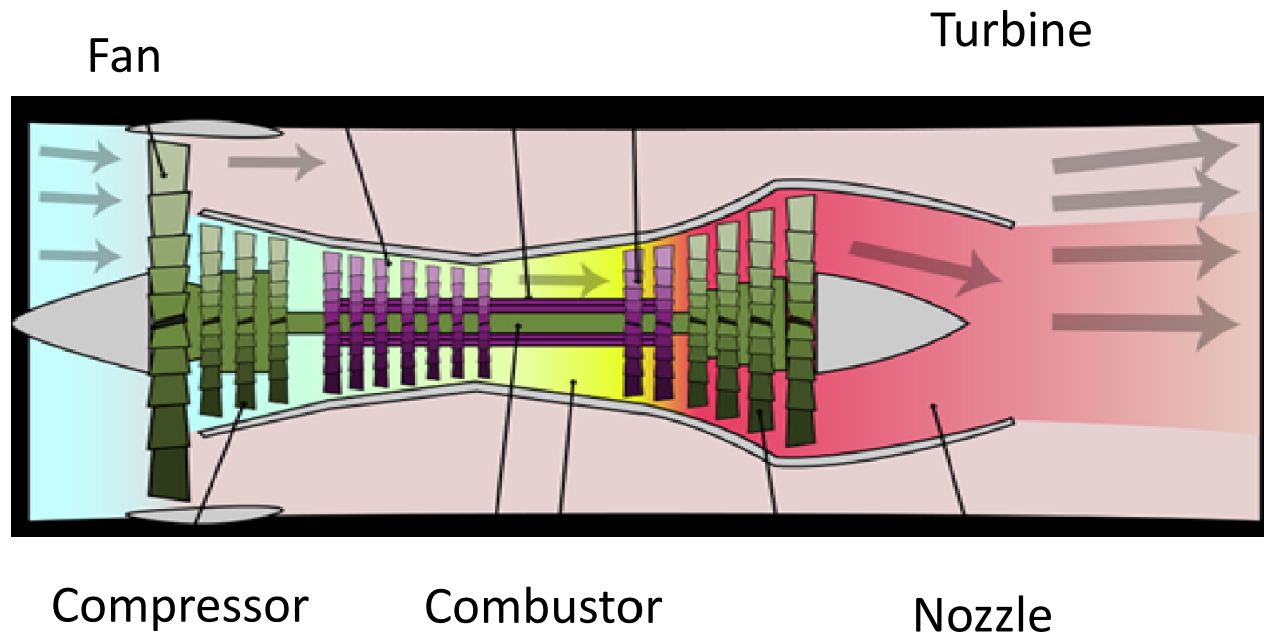
\includegraphics[width = 0.8\textwidth]{img/figure19.png}
    \caption{Jet engine.}
\end{figure}
\subsection{Brayton (or Joule) cycle}
\begin{figure}[H]
    \centering
    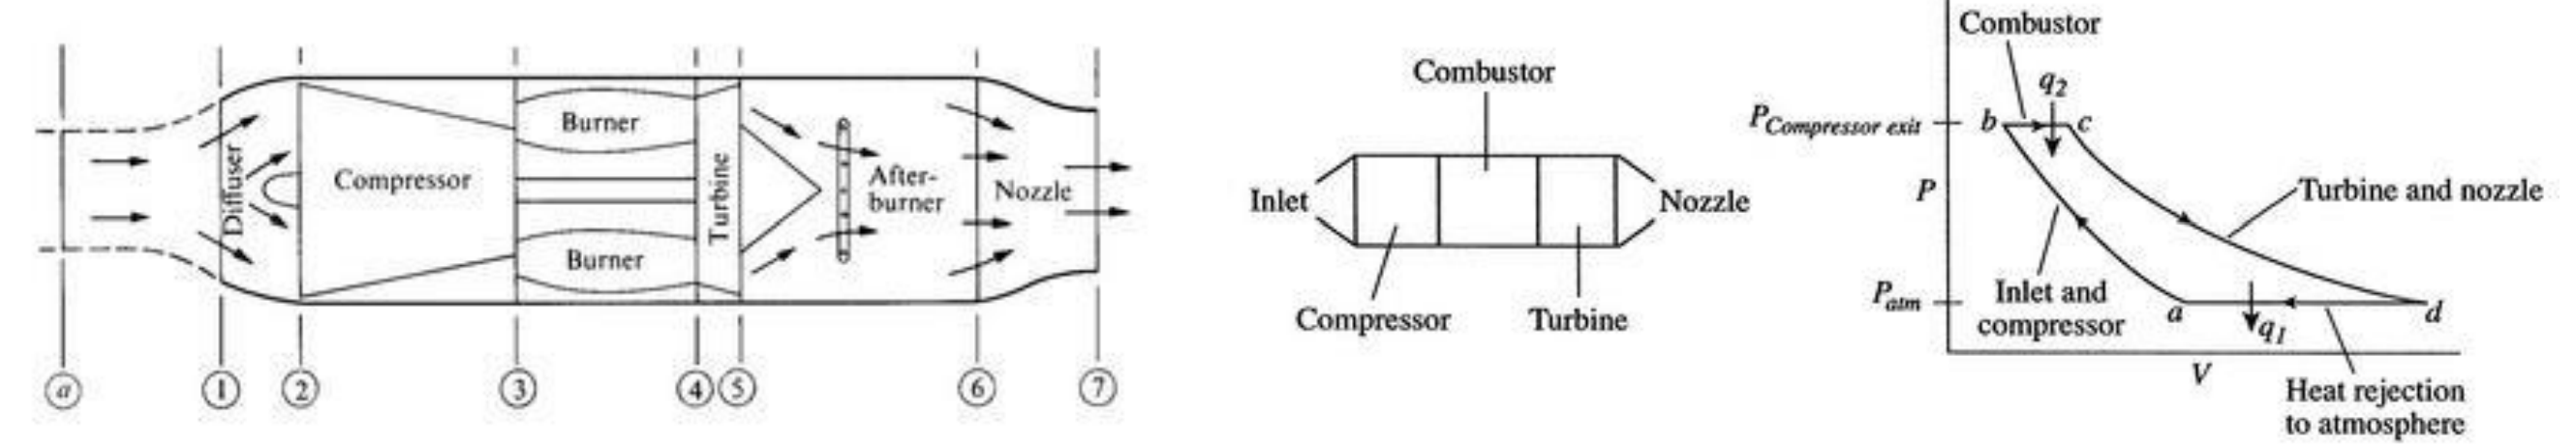
\includegraphics[width = \textwidth]{img/figure20.png}
    \caption{Brayton (or Joule) cycle.}
\end{figure}
\begin{itemize}
    \item a-b: adiabatic, quasi-static (or reversible) compression in the inlet and compressor
    \item b-c: constant pressure fuel combustion (idealised as constant pressure heat addition)
    \item c-d: adiabatic, quasi-static (or reversible) expansion in the turbine and exhaust nozzle, with which we take some work out of the air and use it to drive the compressor and take the remaining work out and use it to accelerate fluid for jet propulsion, or to turn a generator for electrical power generation
    \item d-a: cool the air at constant pressure back to its initial condition
\end{itemize}
\begin{itemize}
    \item \textbf{Fan} - the large spinning fan sucks in large quantities of air. It then speeds this air up and splits it into two parts. One part continues through the ``core'' or centre of the engine, where it is acted upon by the other engine components. The second part ``bypasses'' the core of the engine. It goes through a duct that surrounds the core to the back of the engine where it produces much of the force that propels the airplane forward. The cooler air helps to quiet the engine as well as adding thrust to the engine.
    \item \textbf{Compressor} - the compressor is the first component in the engine core. The compressor squeezes the air that enters it into progressively smaller areas, resulting in an increase in the air pressure. This results in an increase in the energy potential of the air. The squashed air is forced into the combustion chamber. 
    \item \textbf{Combustor} - in the combustor the air is mixed with fuel and then ignited. THis provides a high temperature, high-energy airflow. The fuel burns with the oxygen in the comrpessed air, producing hot expanding gases. The inside of the combustor is often made of ceramic materials to provide a heat-resistant chamber. The temperature can reach \SI{2700}{\degree C}
    \item \textbf{Turbine} - the high-energy airflow coming out of the combustor goes into the turbine, causing the turbine blades to rotate. The turbines are linked by a shaft to turn the blades in the compressor and spin the intake fan at the front. This rotation takes some energy from the high-energy flow that is used to drive the fan and the compressor. The gases produced in the combustion chamber move through the turbine and spin its blades. The turbines of the jet spin around thousands of times. They are on fixed shafts which have several sets of ball-bearings in between them.
    \item \textbf{Nozzle} - the nozzle produces the thrust for the plane. The energy depleted airflow that passed the turbine in addition to the colder air that bypassed the engine core, produces a force when exiting the nozzle that acts to propel the engine, and therefore the airplane, forward. The combination of the hot air and cold air are expelled and produce an exhaust, which causes a forward thrust. The nozzle may be preceded by a mixer, which combine the high temperature air coming from the engine core with the lower temperature air that was bypassed in the fan. The mixer helps to make the enginer quieter. 
\end{itemize}
\subsection{Typical values}
\begin{figure}[H]
    \centering
    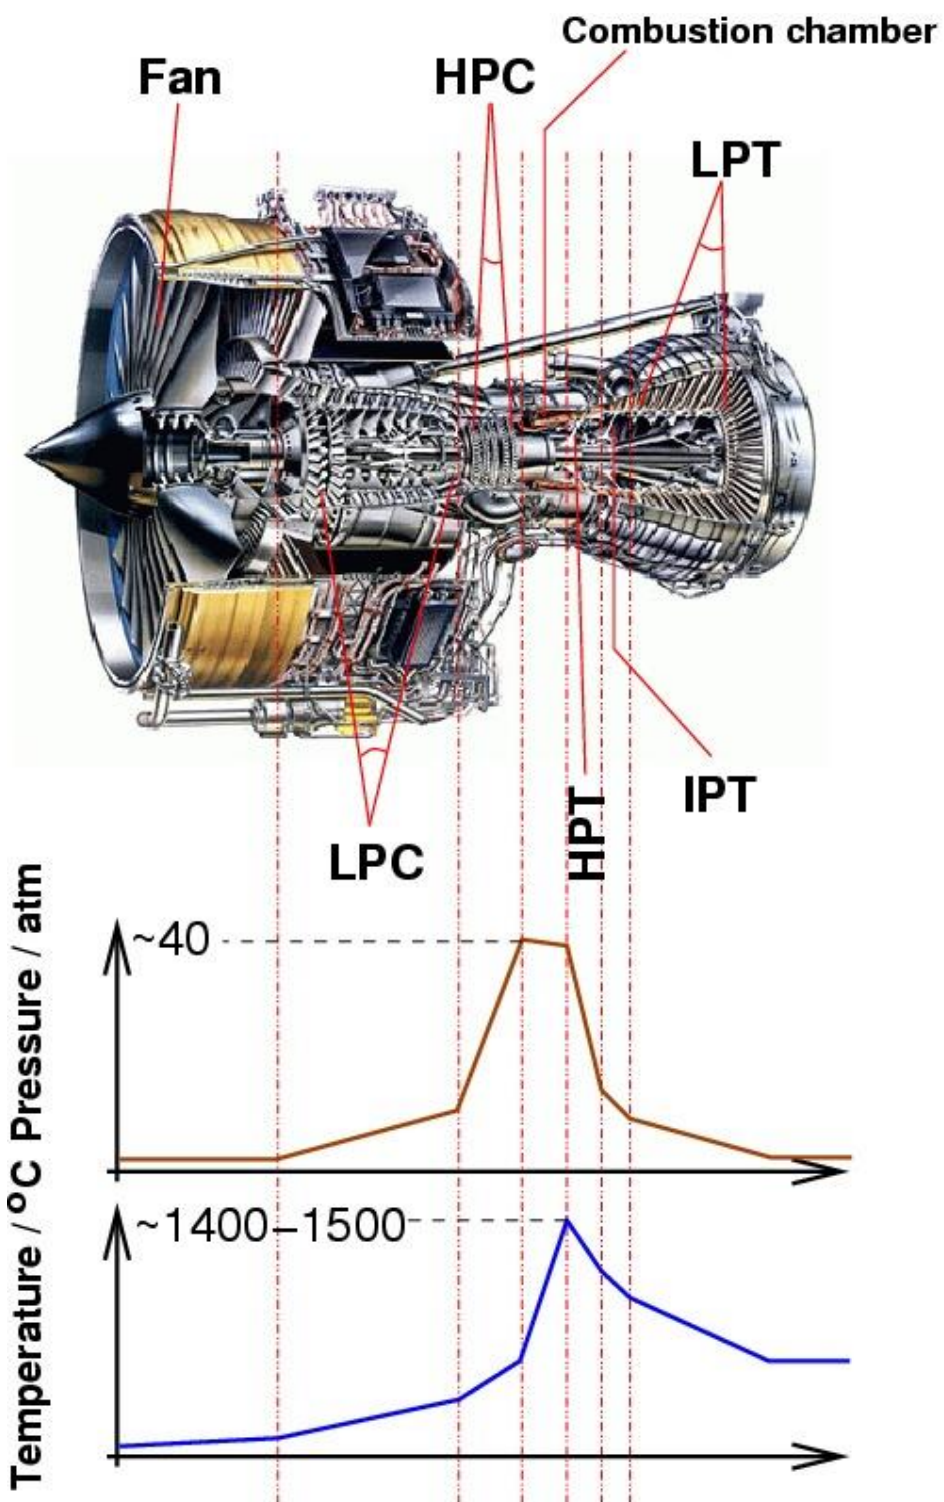
\includegraphics[width =0.5\textwidth]{img/figure21.png}
    \caption{Typical temperature values for different stages of cycle in bypass gas-turbine engine.}
\end{figure}
\begin{table}[H]
    \centering
    \begin{tabular}{@{}ll@{}}
        \toprule
        \textbf{Metal} & \textbf{Melting point}\\
        \midrule
        Titanium & \SI{1668}{\degree C}\\
        Nickel & \SI{1455}{\degree C}\\
        Steel & \SI{1370}{\degree C}\\
        \bottomrule
    \end{tabular}
    \caption{Table to show melting points of various metals used in bypass gas-turbine engines.}
\end{table}
Combustion at about 1800-\SI{1900}{\degree C}. Large centrifugal acceleration \SI{25000}{rpm} for large engines \SI{500000}{rpm} for micro gas turbine. Higher temperature makes the thermodynamic efficiency greater (about 60\%). Combustion temperature is above melting point of metals. 
\begin{table}[H]
    \centering
    \begin{tabular}{@{}ll@{}}
        \toprule
        \textbf{Fuel} & \textbf{Combustion temperature}\\
        \midrule
        Methane (in air) & \SI{1950}{\degree C}\\
        Hydrogen (in air) & \SI{2110}{\degree C}\\
        Propane (in oxygen) & \SI{2880}{\degree C}\\
        \bottomrule
    \end{tabular}
    \caption{Table to show combustion temperatures of various fuels.}
\end{table}
\subsubsection{Meeting the needs}
\begin{enumerate}
    \item Choice of material
    \item Manufacturing technique
    \item Design
\end{enumerate}
\begin{figure}[H]
    \centering
    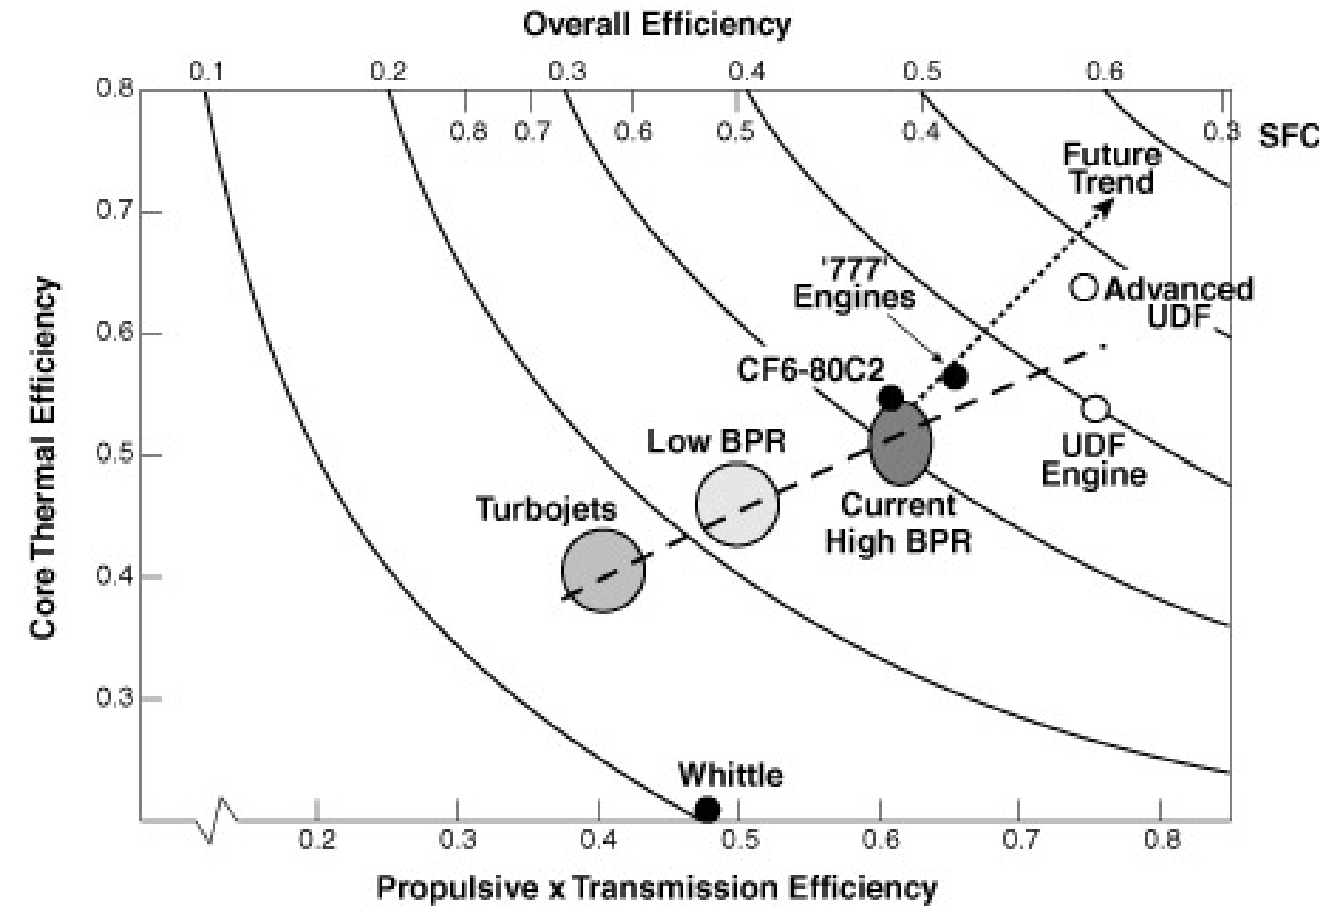
\includegraphics[width =0.8\textwidth]{img/figure22.png}
    \caption{Efficiencies of various gas-turbine engines.}
\end{figure}
\subsection{Material selection}
Considerations:
\begin{enumerate}
    \item Strength and weight: titanium
    \item Temperature: major constraint is the material selection for the hot section (combustor and turbine) of the engine
\end{enumerate}
The need for better materials spurred much research in the field of alloys and manufacturing techniques, and that research resulting in a long list of new materials and methods that make modern gas turbines possible. One of the earliest of these was Nimonic 90 (nickel-based, high-temperature, low-creep superalloys Ni 54\%, Cr 18-21\%, Co 15-21\%, Ti 2-3\%, Al 1-2\%).

The development of superalloys in the 1940s and new processing methods such as vacuum induction melting in the 1950s greatly increased the temperature capability of turbine blades. Further processing methods like hot isostatic pressing improved the alloys used for turbine blades and increased turbine blade performance. Modern turbine blades often use nickel-based superalloys that incorporate chromium, cobalt and rhenium.
\begin{figure}[H]
    \centering
    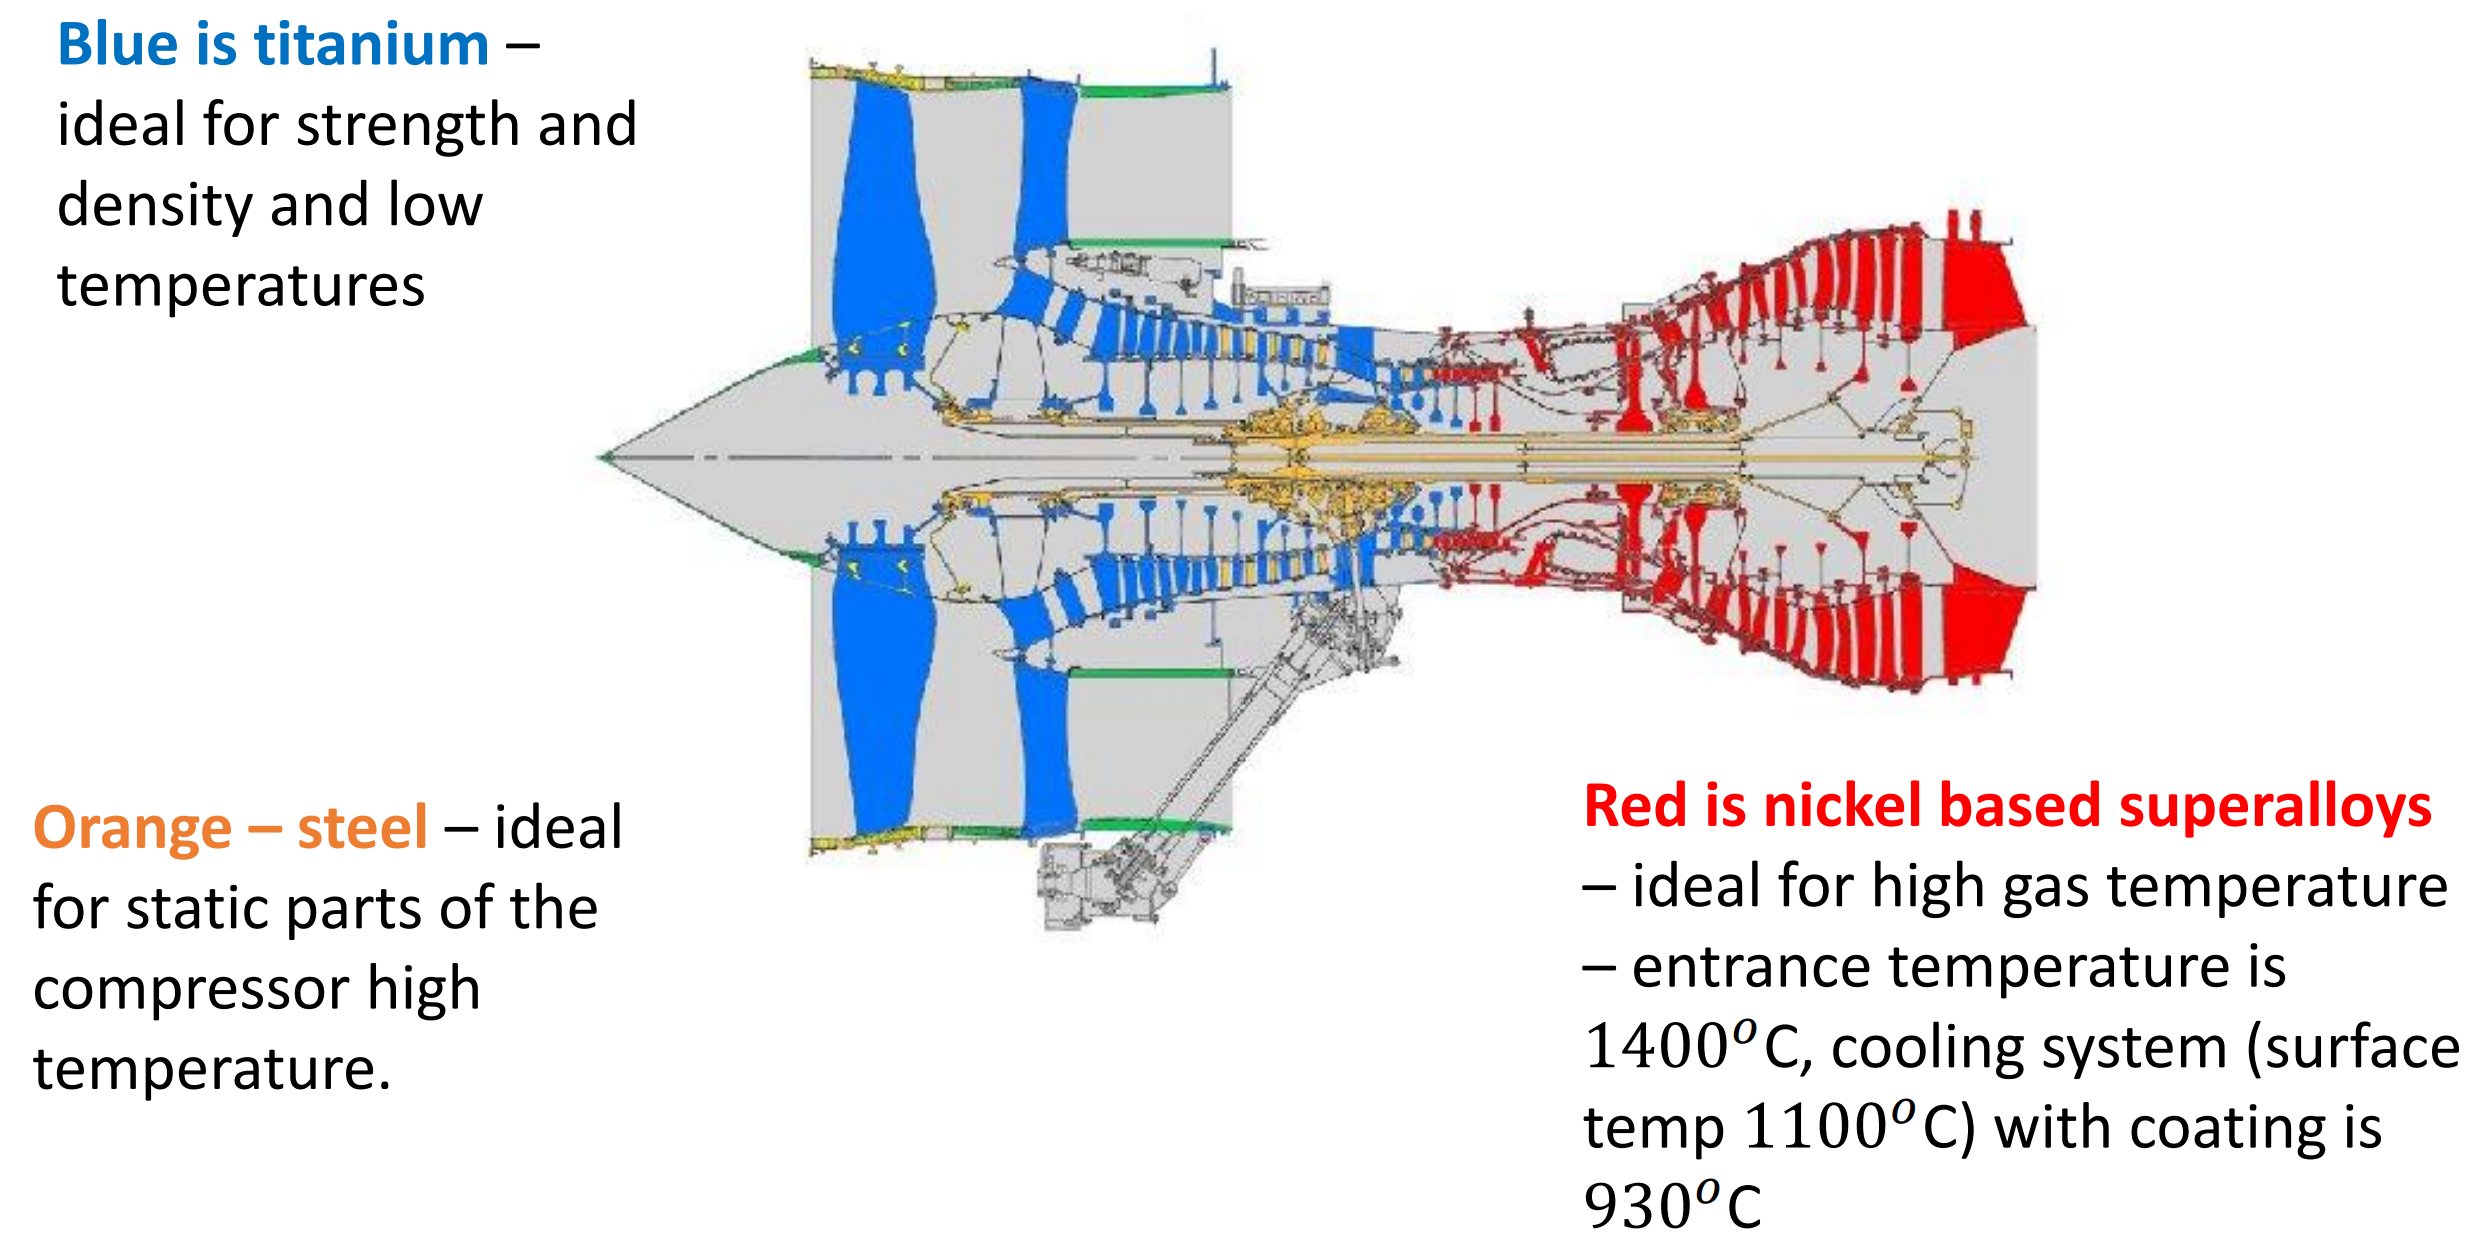
\includegraphics[width =\textwidth]{img/figure23.png}
    \caption{Usage of different alloys within the engine.}
\end{figure}
\begin{figure}[H]
    \centering
    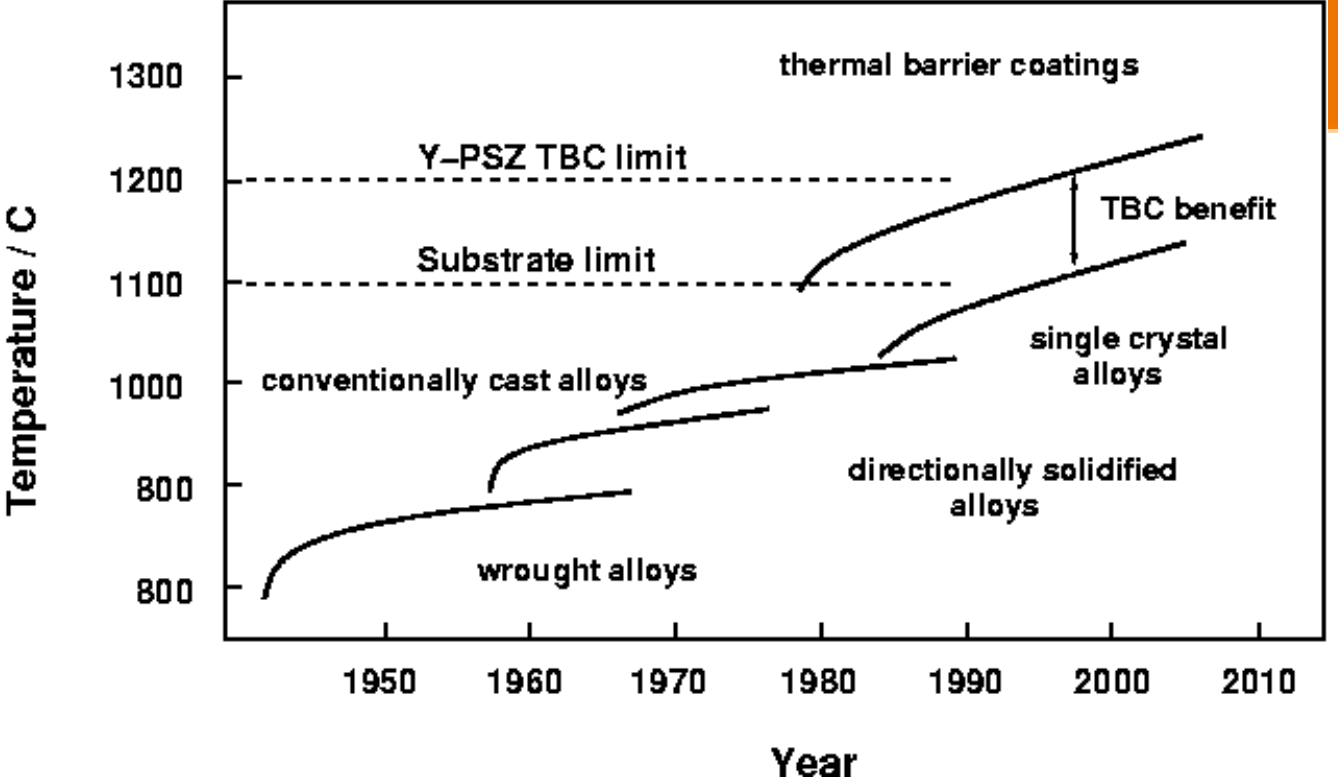
\includegraphics[width =0.8\textwidth]{img/figure24.png}
    \caption{Development of alloys.}
\end{figure}
Titanium - good for weight and strength (poor with heat).

Alloy improvement, directional and single-crystal solidifcation have contributed significantly, but arguably, the empahsis has been shifted to coating systems which have allowed an increase of gas temperatures up to \SI{1100}{\degree C}. Coatings in gas turbines serve a variety of purposes. A first requirement to operate turbines at higher temperatures was, of course, improved strength. Unfortunately, these conditions also mean severe oxidation / corrosion problems, and to make things worse, the improvement in mechanical properties of the base alloys was made at the expense of environmental resistance. 

The first purpose of coatings was to improve poor oxidation resistance of the base alloy (aluminide, Pt-aluminide, MCrAlY). A second type of coatings applied to high-temperature parts are known as thermal barrier coatings (TBC). These are ceramic coatings with very low thermal conductivity and thin (\SI{200}{\micro\meter}). Drop of 100-\SI{300}{\degree C} between the gas and metal surface temperatures but are `oxygen transparent' and do not prevent oxidation of the underlying substrate.
\subsection{Manufacturing process}
Aside from the alloy improvements, a major breakthrough was the development of directional solidification (DS) and single crystal (SC) production methods. These methods help greatly increase strength against fatigue and creep by aligning grain boundaries in one direction (DS) or by eliminating grain boundaries altogether (SC).

Recent generations of superalloys for single crystal turbine blades contain relatively high percentages of refractory elements such as Ta, W or Re which enhance the high-temperature mechanical properties. 

This is done at the expense of Cr and Al. Given the severe environmental conditions in which the blades operate, the removal of the elements (beneficical for oxidation resistance) implies even greater degradation problems. 

To reduce the oxidation corrosion resistance, an external coating is applied to the blades. Its purpose is to allow for the growth of a resistant oxide layer. Of all possible oxides $\alpha$-Al$_2$O$_3$ offers excellent protection and very low growth rates (in a minority of cases, Cr oxides are preferred). The composition of the coating must therefore be chosen carefulyl so as to ensure growth of $\alpha$-Al$_2$O$_3$.
\begin{figure}[H]
    \centering
    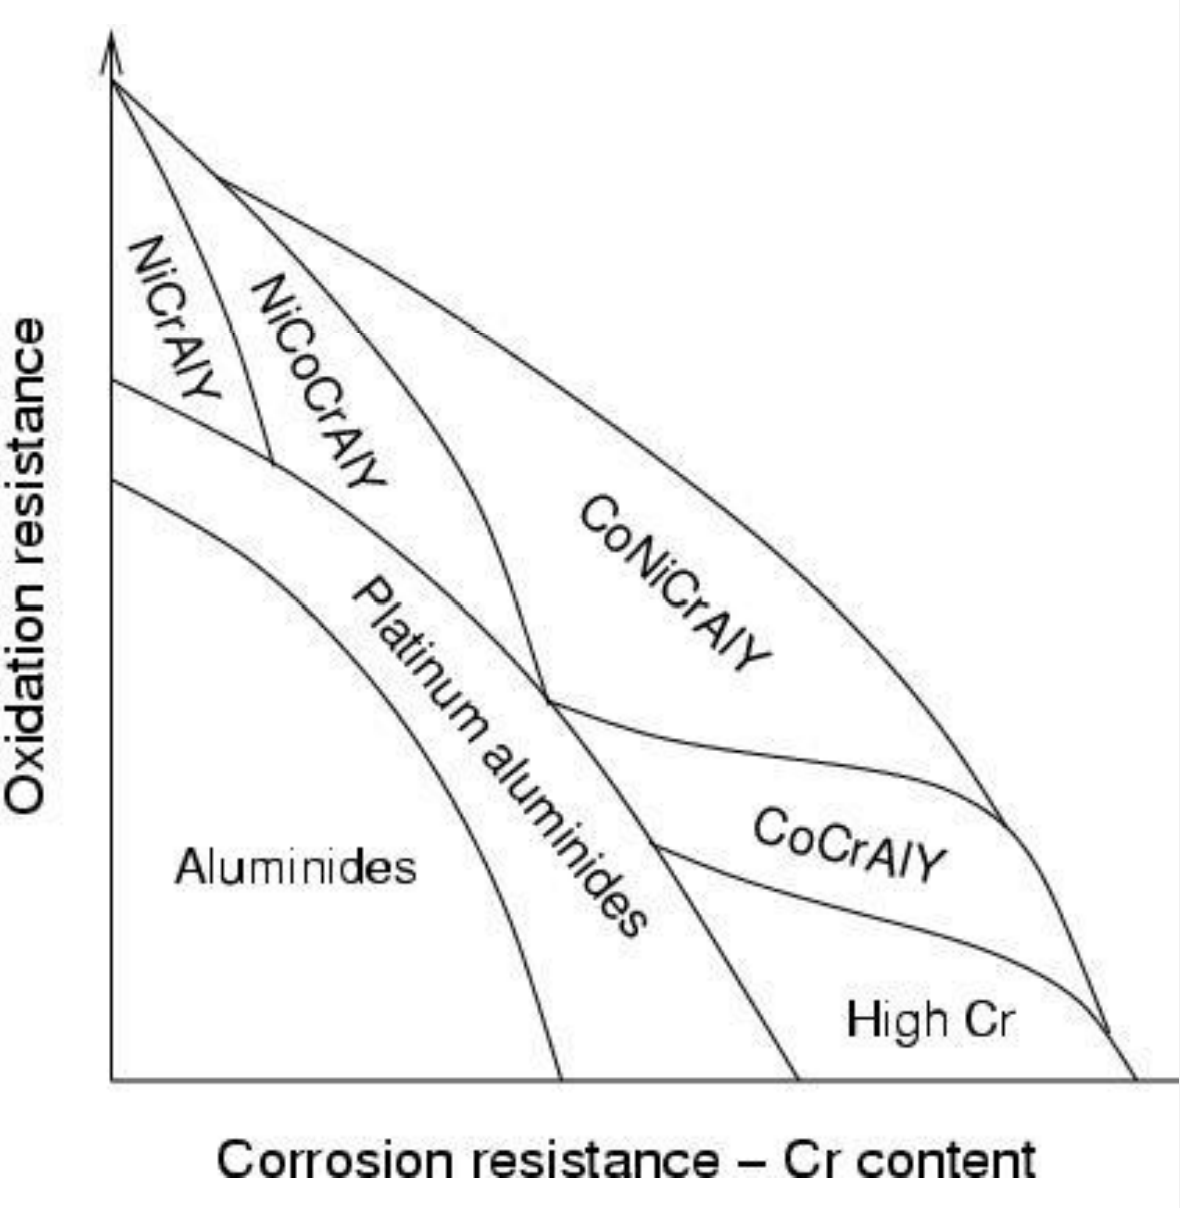
\includegraphics[width =0.6\textwidth]{img/figure25.png}
    \caption{Oxidation and corrosion resistance of different alloys.}
\end{figure}
\begin{figure}[H]
    \centering
    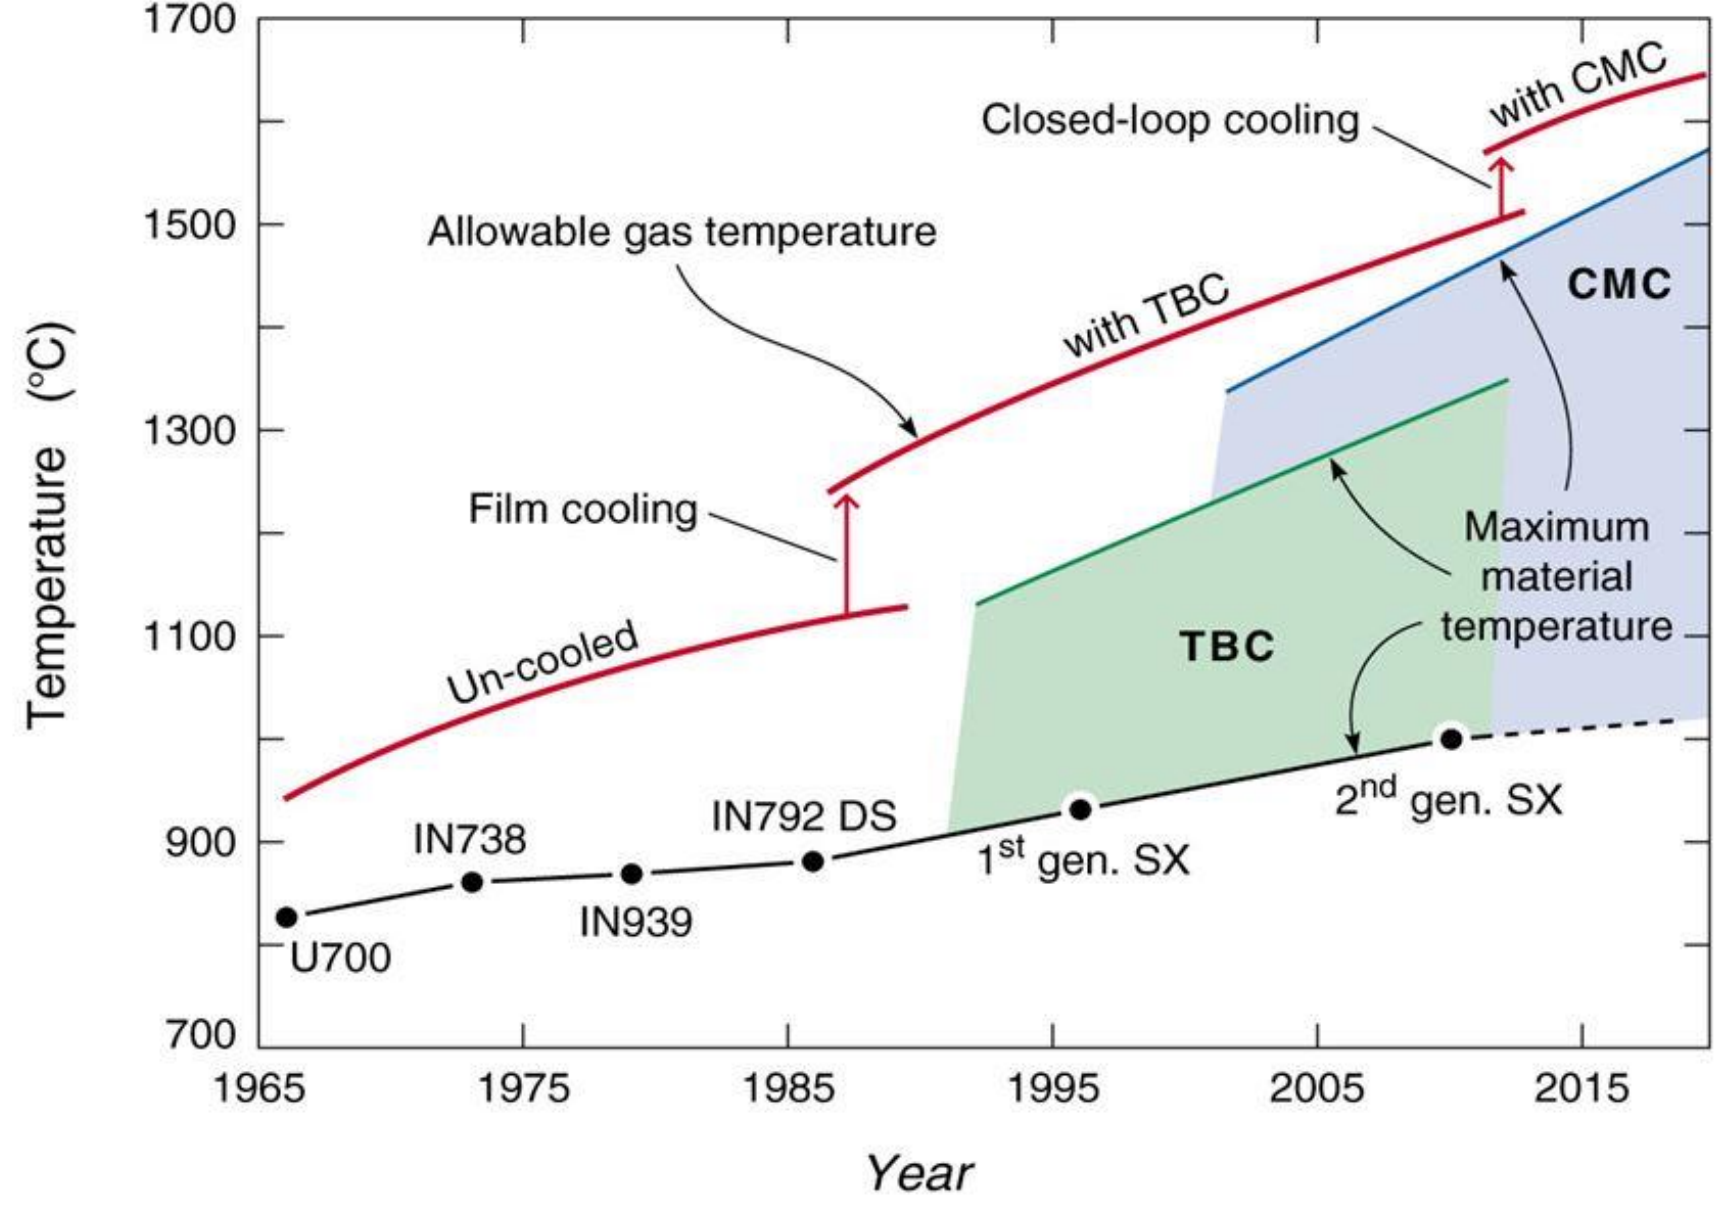
\includegraphics[width =0.8\textwidth]{img/figure26.png}
    \caption{Temperature resistance of TBCs and CMCs over the years.}
\end{figure}
TBC - thermal barrier coating. CMC - ceramic matrix composite.
\subsection{Thermal barrier coating}
Thermal barrier coatings (TBC) are advanced materials systems usually applied to metallic surfaces, such as on gas turbine or aero-engine parts, operating at elevated temperatures, as a form of exhaust heat management. These \SI{100}{\micro\meter} to \SI{2}{mm} coatings serve to insulate components from large and prolonged heat loads by utilising thermally insulating materials which can sustain an appreciable temperature difference between the load-bearing alloys and the coating surface.
\begin{figure}[H]
    \centering
    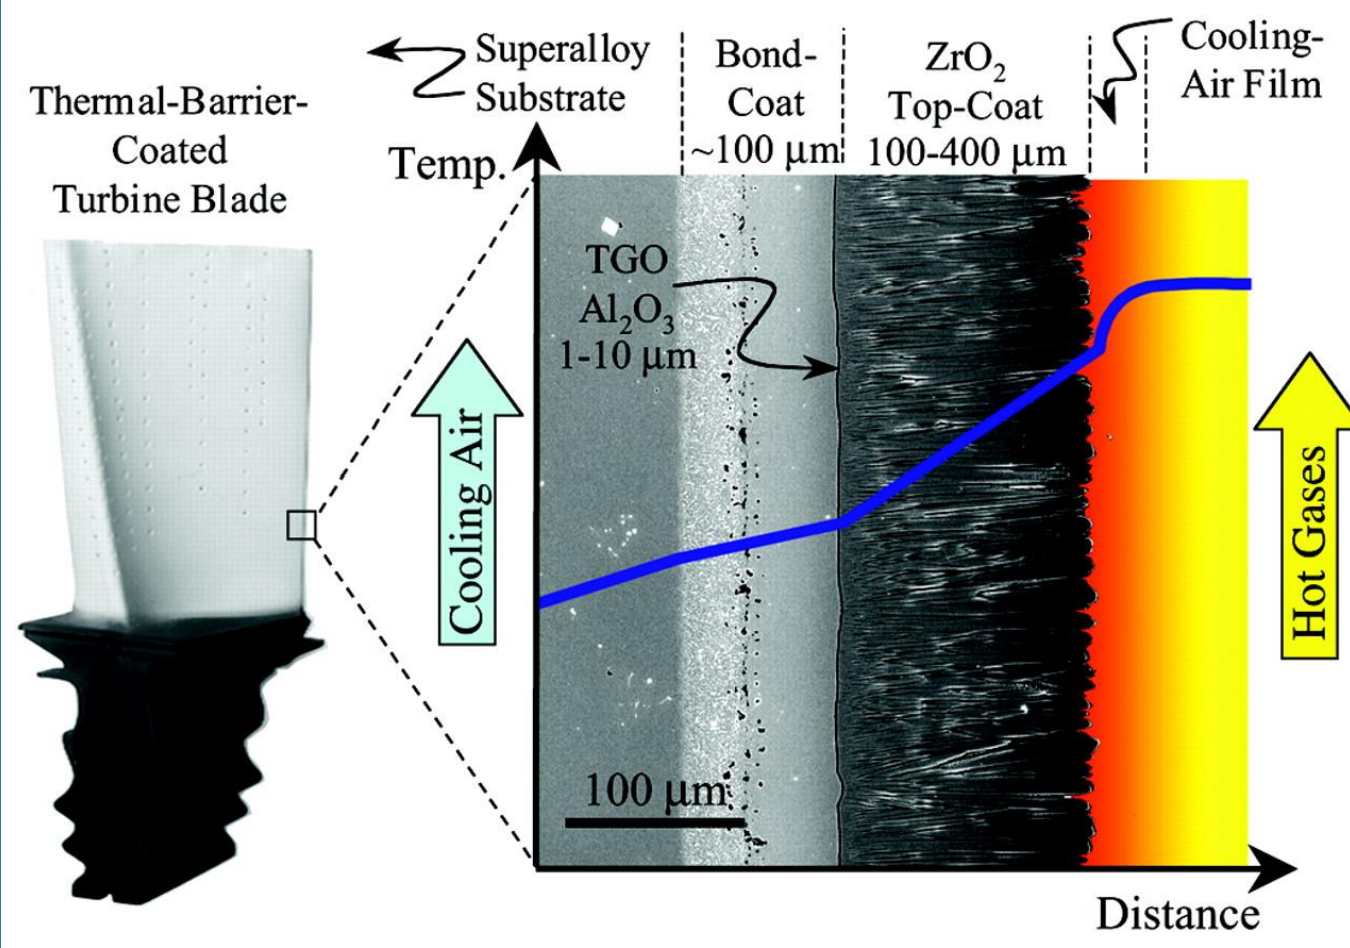
\includegraphics[width =0.6\textwidth]{img/figure27.png}
    \caption{Thermal barrier coatings (TBCs).}
\end{figure}
Four layers:
\begin{enumerate}
    \item The metal substrate
    \item Metallic bond coat
    \item Thermally-grown oxide (TGO)
    \item Ceramic topcoat. The ceramic topcoat is typically composed of yttria-stabilised zirconia (YSZ) which is desirable for having very low of conductivity while remaining stable at nominal operating temperatures typically seen in applications. This ceramic layer creates the largest thermal gradient of the TBC and keeps the lower layers at a lower temperature than the surface.
\end{enumerate}
\begin{figure}[H]
    \centering
    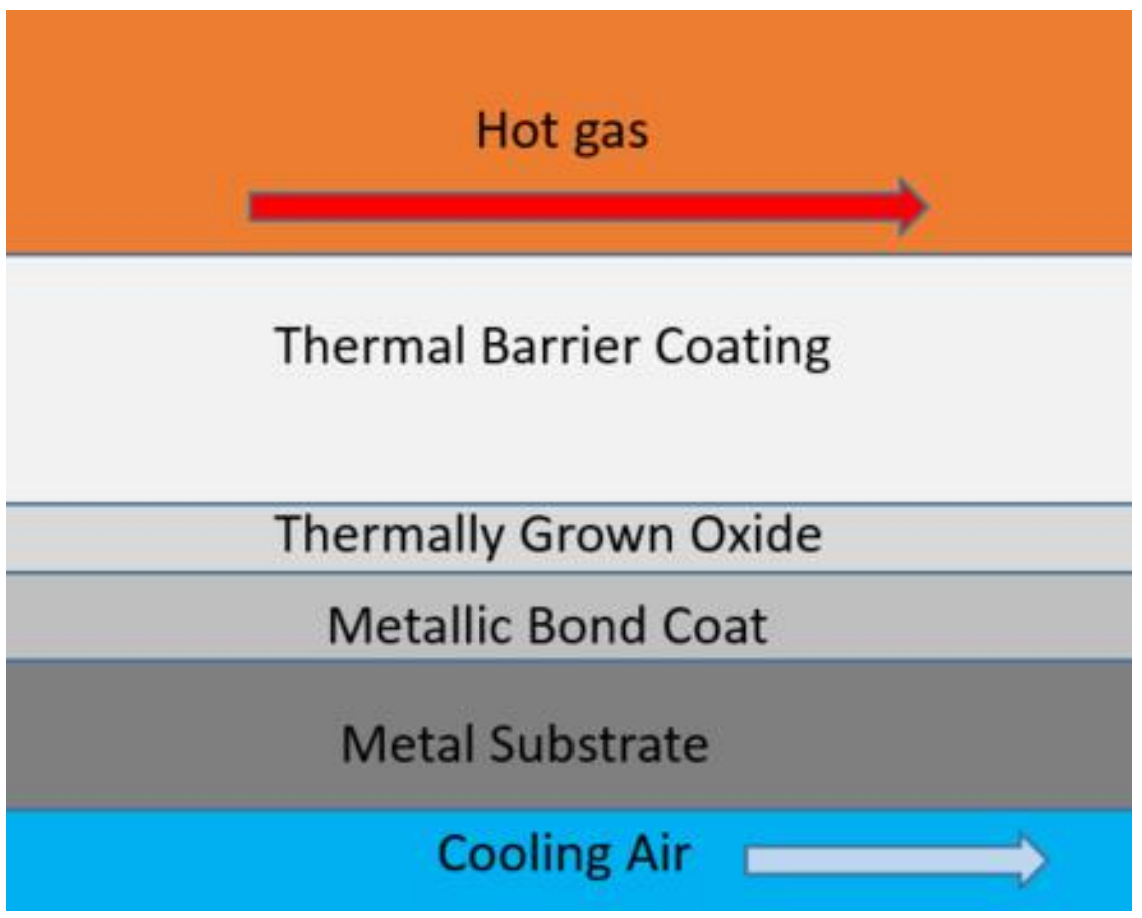
\includegraphics[width =0.6\textwidth]{img/figure28.png}
    \caption{Thermal barrier coating composition.}
\end{figure}
TBCs improved corrosion and oxidation resistance, both which became greater concerns as temperatures increased. First TBCs (1970s) were aluminide coatings. Ceramic coatings in 1980s which decreased turbine blade temperature by about \SI{90}{\degree C}, improve blade life, almost doubling the life of turbine blades in some cases.
\chapter{Large Spatial and Temporal Variations of Temperature}
\section{Introduction}
Many different engineering materials are subject to intense heating and cooling in localised regions. As with our previous discussion about materials, the temperature might be spatially or temporally variable. In Lecture 13, we looked at the thermoelastic response of materials subject to small temperature variations. Their response can be dealt with via a linear elastic model. In this chapter, we look at the effect of a large temperature applied to a material which are sufficient to generate a plastic response and how the spatial and temporal variation affects the material properties.

The incandescent light build initially failed due to the thermal fatigue and melting problems. This was largely a material selection and corrosion problem. Turning a light on and off generates enormous thermal stresses, but keeping it on continuously is fine. The filament is made of tungsten which has a high melting point. The inert gases around the filament stop evaporation. Most of energy dissipated is thermal.
\subsubsection{Types of heating processes}
\begin{itemize}
    \item \textbf{Mechanical heating}, usually by friction
    \item \textbf{Electrical heating}, using the material itself for energy release (e.g. induction heating), or more commonly by external means with an electrical resistance made of Nichrome (60\% Ni, 25\% Fe, 15\% Cr) or Kanthal (70\%, 24\% Cr, 5\% Al)
    \item \textbf{Radiation heating}, either with microwaves, infrared radiation from heated wires protected inside a quartz-glass (wires can be made of tungsten, carbon, Kanthal or Nichrome; naked Nichrome coiled wire was also used in the past), or using visible radiation (with a laser).
    \item \textbf{Chemical heating}, mainly by combustion, but also by hydrogen formation after atomic hydrogen is produced in an electric car, for instance.
    \item \textbf{Nuclear heating}, by nuclear fission or fusion
\end{itemize}
\begin{figure}[H]
    \centering
    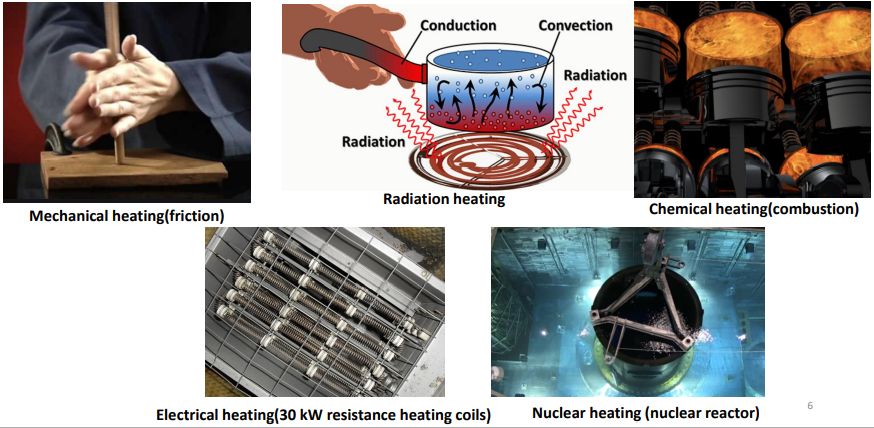
\includegraphics[width = 0.8\textwidth]{img/figure41.png}
    \caption{Heating processes.}
\end{figure}
\begin{figure}[H]
    \centering
    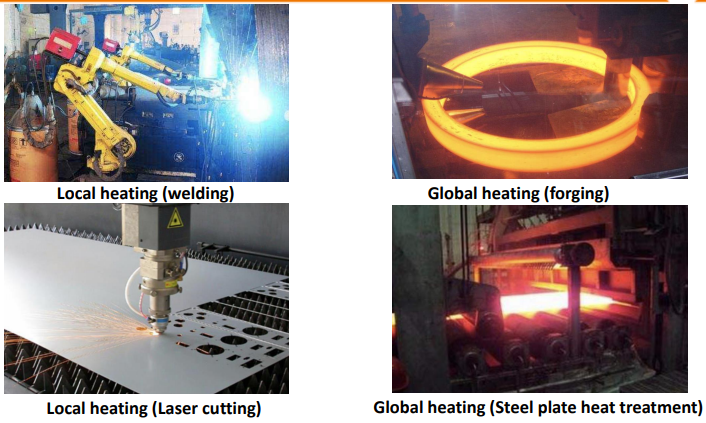
\includegraphics[width = 0.8\textwidth]{img/figure40.png}
    \caption{Localised heating processes.}
\end{figure}
\section{Practical application of heat to a material}
Any time a material is heated, the heat is applied spatially and temporally. The characteristics scales have quite different effects on the material and structure.
\begin{table}[H]
    \centering
    \begin{tabular}{@{}lll@{}}
        \toprule
             & \textbf{Localised} & \textbf{Uniform} \\
        \midrule
        Slow & Welding            & Heat treatment   \\
        Fast & Thermal shocking   & Quenching        \\
        \bottomrule
    \end{tabular}
    \caption{Spatial and temporal heat application.}
\end{table}
\subsection{Welding}
\begin{itemize}
    \item TIG - Tungsten gas - electrode is tungsten. You do not need a metal filter. Need a gas tank to protect the weld - most often applied to stainless steels and light metals
    \item Flux-cored Arc Welding - similar to MIG. Uses a wire to serve as an electrode and a metal filler fed through the wand. Wire has a flux that creates the gas shield. Tends to have slag left so usually needs a clean-up
    \item Stick (Shielded Metal Arc Welding). Replaceable electrode stick t hat forms the filler metal. Arc is created at the end of the electrode. Stick is coated in flux that protects the metal from oxidation
    \item MIG welding (metal inert gas). Filler metal is consumable wire that acts as an electrode
    \item Laser beam welding - used on a few metals with laser providing the heat
    \item Plasma Arc Welding - uses a smaller arc with a high pressurised gas that is ionised and electrically conductive
\end{itemize}
Small amount of molten metal are introduced in the gap between two components to solidify the body. Major regions are:
\begin{enumerate}
    \item Fusion where the parts of the metal have melted and combined with filler material
    \item Heat affected zone - region next to steel that have undergone microstructural changes
\end{enumerate}
\subsection{Friction welding}
\url{https://www.youtube.com/watch?v=RTEP9QdTn5k}
\begin{figure}[H]
    \centering
    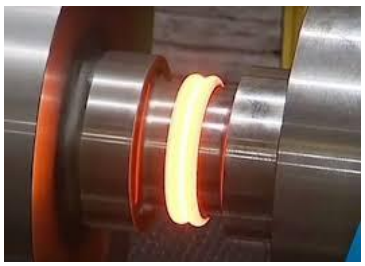
\includegraphics[width = 0.8\textwidth]{img/figure44.png}
    \caption{Friction welding.}
\end{figure}
\subsection{Radiation heating}
\begin{figure}[H]
    \centering
    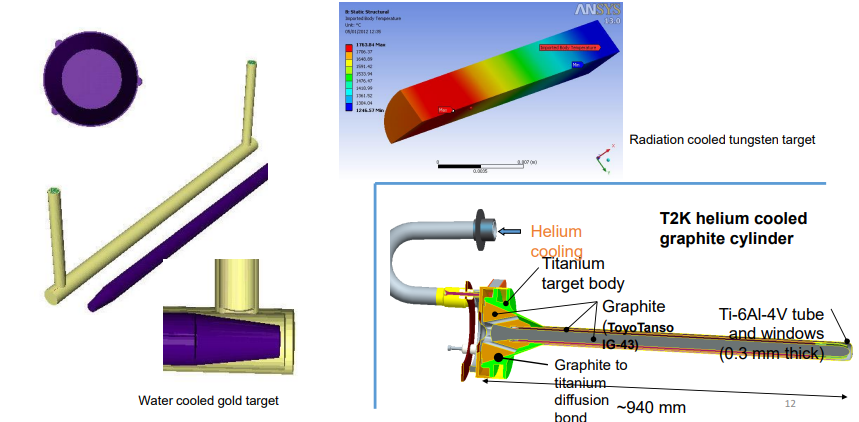
\includegraphics[width = 0.8\textwidth]{img/figure42.png}
    \caption{Radiation heating.}
\end{figure}
\subsection{Laser heating}
\begin{figure}[H]
    \centering
    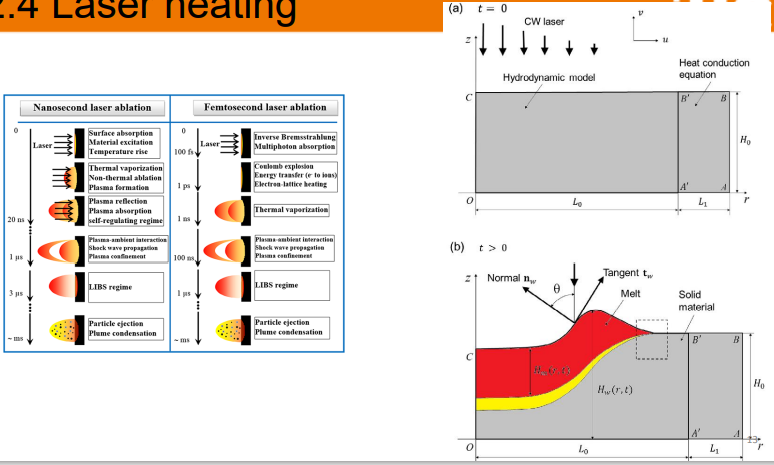
\includegraphics[width = 0.8\textwidth]{img/figure45.png}
    \caption{Laser heating.}
\end{figure}
\begin{figure}[H]
    \centering
    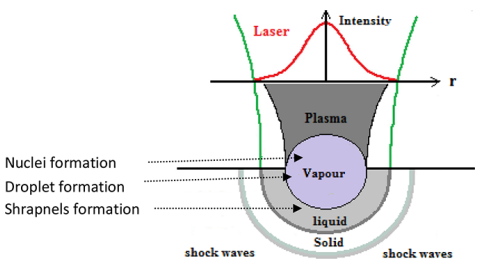
\includegraphics[width = 0.8\textwidth]{img/figure46.png}
    \caption{Close-up of laser heating.}
\end{figure}
\begin{figure}[H]
    \centering
    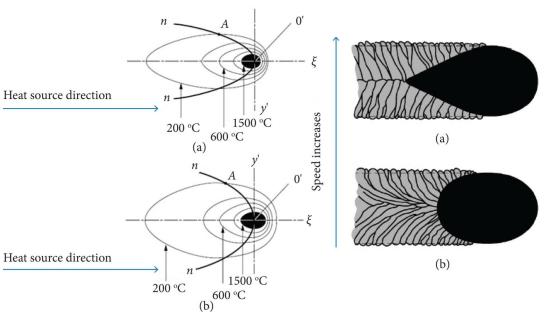
\includegraphics[width = 0.8\textwidth]{img/figure47.png}
    \caption{Close-up of laser heating.}
\end{figure}
The heat spreads out through diffusion from a moving source. The temperature distribution can be analysed using simple mathematical models of a moving source and this is discussed in Worksheet 15.
\section{Structural changes in the matter}
\url{https://www.youtube.com/watch?v=uG35D_euM-0&authuser=0}
\subsection{Microstructural changes}
Metals are comprised of a symmetrical structure of atoms known as an allotrope. Heating the metal will displace atoms from their position and the displaced atoms form a new structure. This process is known as allotropic phase transformation. Allotropic phase transformation alters the hardness, strength and ductility of the metal. The most important allotropic phase transformation is undergone by iron. When iron is heated past \SI{912}{\degree C} it is able to absorb more carbon which is essential for the manufacture of stainless steel.
\begin{figure}[H]
    \centering
    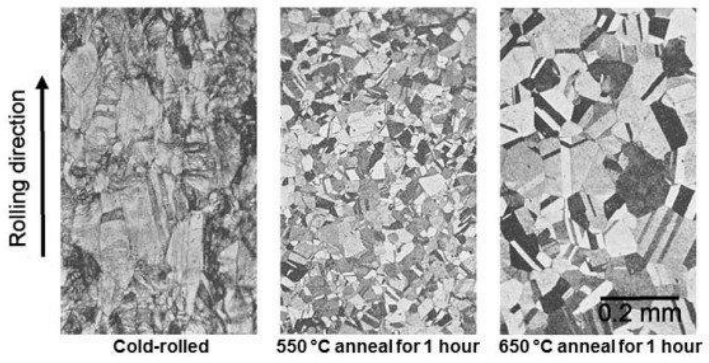
\includegraphics[width = 0.8\textwidth]{img/figure43.png}
    \caption{Effect on microstructure from cold rolling and then annealing.}
\end{figure}
\subsubsection{Heat treatment}
\textbf{Annealing} is used to soften metals including iron, steel, copper, brass and silver. The process involves heating the metal to a specific temperature then allowing it to cool slowly at a controlled rate. Annealing alters the physical and chemical properties of the metal to increase ductility and reduce hardness. This facilitates shaping, stamping or forming processes, and allows the metal to be cut more easily. Annealing also enhances electrical conductivity.

\textbf{Normalising} is applied to alloys to provide uniformity in grain size and composition. The metal is heated to a predefined temperature then cooled by air. The resulting metal is free of undesirable impurities and exhibits greater strength and hardness. Normalising is often used to produce a harder and stronger steel, albeit one that is less ductile than that produced by annealing. Typically, the normalising process is performed on materials that will be subjected to machining, because the process has improved this attribute.

\textbf{Hardening} is applied to steel and other alloys to improve their mechanical properties. During hardening, the metal is heated at a high temperature and this temperature is maintained until a proportion of carbon has been dissolved. Next the metal will is quenched, which involves rapidly cooling it in oil or water. Hardening will produce an alloy which has high strength and and wear resistance. However, hardening will also increase brittleness and is not suitable for engineering applications. When there is a need to have the surface of the component hard enough to resist wear and erosion, while maintaining ductility and toughness to withstand impact and shock loading - surface hardening would be used.

\textbf{Tempering} is applied to steel where ductility is desired. Untempered steel is very hard but too brittle for most practical applications. Tempering is a low temperature heat treatment process normally performed after hardening (neutral hardening, double hardening, atmospheric carburising, carbonitriding, or induction hardening) in order to reach a desired hardness/toughness ratio. the process involves heating steel to a lower temperature to reduce some of the excess hardness. The metal is then allowed to cool in still air which results in a tougher and less brittle steel.
\subsection{Macroscopic changes}
Large temperature variations lead to inelastic and non-recoverable deformations. For plastic deformation require about 0.2\% residual strain. Since the strain generated a temperature difference of $\Delta T$ scales as $\epsilon \sim \Delta T \alpha$. With a typical value of a $\alpha \sim \SI{1e-5}{\per\kelvin}$, we only need $\Delta T \sim \SI{200}{\kelvin}$ to generate this strain. Large temperatures leads to melting, rearrangement of bonds and this is what is used in casting and welding. Ductile and malleable materials can absorb changes while brittle materials fracture.
\section{Soldering, brazing, welding}
\begin{itemize}
    \item Soldering is a low-temperature process (60-\SI{400}{\degree C}) that uses a low-melting metal (a base of tin combined with lead, silver, antimony, bismuth, indium) to join similar or dissimilar metals; it is mainly used in electronic boards
    \item Brazing is a mid-temperature process (450-\SI{1200}{\degree C}) that uses a high-melting metal (a base of silver combined with nickel, copper, zinc) to join similar or dissimilar metals; it is mainly used in copper piping and jewellery
    \item Welding is a high temperature process (800-\SI{2000}{\degree C}) that uses a powerful heat source to locally melt and join similar metals; it is mainly used in iron and steel work
\end{itemize}
\subsubsection{Influence of localised heating}
Close to the weld there is a heat affected region where the microstructure is affected by the heat. The metal in this area is generally weaker than the base material and the fusion zone. This is where the residual stresses are found.
\begin{figure}[H]
    \centering
    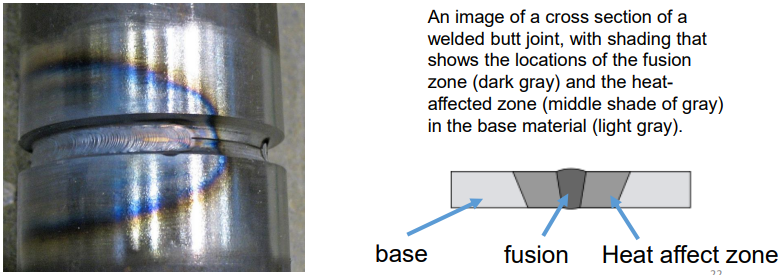
\includegraphics[width = 0.8\textwidth]{img/figure48.png}
    \caption{Influence of localised heating on a weld.}
\end{figure}
\subsubsection{Heat affected zone}
This is the ring that surrounds the weld which affects the alloy. If thermal diffusivity is high, cooling rate is high so the HAZ is smaller. If thermal diffusivity is low, cooling rate is low so the HAZ is bigger. Other measures are used, such as rate of heat input for weld where:
\begin{equation}
    Q = \frac{60VI}{1000U}\times \textrm{efficiency}
\end{equation}
\begin{itemize}
    \item $Q$ is the heat input (\si{\kilo\joule\per\milli\meter})
    \item $VI$ is the electrical power
    \item $U$ is the speed of the weld
\end{itemize}
Usually we need $Q \approx 10-\SI{25}{\kilo\joule\per\milli\meter}$.
\begin{table}[H]
    \centering
    \begin{tabular}{@{}ll@{}}
        \toprule
        \textbf{Weld} & \textbf{Efficiency} \\
        \midrule
        PAW           & 0.46                \\
        GTAW          & 0.65                \\
        Gas metal arc & 0.83                \\
        \bottomrule
    \end{tabular}
    \caption{Welding efficiencies.}
\end{table}
\subsubsection{Thermoplastic shrinkage}
When a plate is heated, there is an elastic convex deformation that fades as it is cooled and a plastic concave deformation. This is exploited in ship manufacturing techniques to create curved sheets.
\begin{figure}[H]
    \centering
    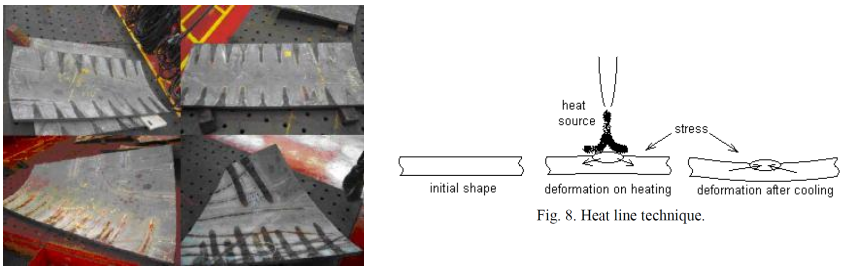
\includegraphics[width = 0.8\textwidth]{img/figure49.png}
    \caption{Thermoplastic shrinkage.}
\end{figure}
\begin{figure}[H]
    \centering
    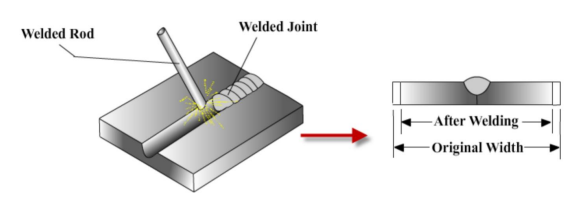
\includegraphics[width = 0.8\textwidth]{img/figure50.png}
    \caption{Weld shrinkage.}
\end{figure}
Weld shrinkage - generated by localised stresses caused by heating and distortion of the heated material. Usually leads to transverse and longitudinal shrinkage.
\subsubsection{Process of plate heating}
The process is known as heat line technique or line heating method of plate bending; it is applied mainly to mild-steel plates, and was started in the 1970s in shipbuilding. It consists of the following steps.
\begin{enumerate}
    \item Initial heating. It forces the heated mass to expand against the rest of the material, creating great stresses and a very small convex elastic deformation due to the temperature gradient
    \item High heating. Up to \SI{1200}{\kelvin} (but usually limited to $<$\SI{995}{\kelvin} to avoid the mild-steel phase transition). It lowers the strength of the heated mass so much, that plastic-yield takes place, that the side material forces the heated mass to bulge in the hottest region
    \item After cooling. Forced cooling (usually by water) increases the temperature gradient that forces the heated mass to recover its original strength but not its original shape, because the plastic deformation is not reversible, causing a shrinkage that pulls in from the rest of the material (i.e. in the whole it is not a thermal push but a thermal pull), causing a concave bending (and perhaps some cracks), and minor in-plane deformations due to the point-wise application (instead of the whole line at a time).
\end{enumerate}
\begin{figure}[H]
    \centering
    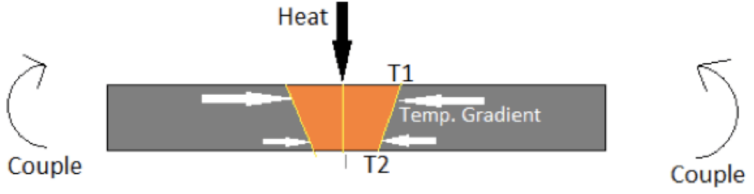
\includegraphics[width = 0.8\textwidth]{img/figure51.png}
    \caption{Plate heating.}
\end{figure}

%\newpage
%\bibliographystyle{unsrtnat}
%\bibliography{Refs.bib}
%\appendix
\chapter{Plots}
\begin{figure}[H]
    \centering
    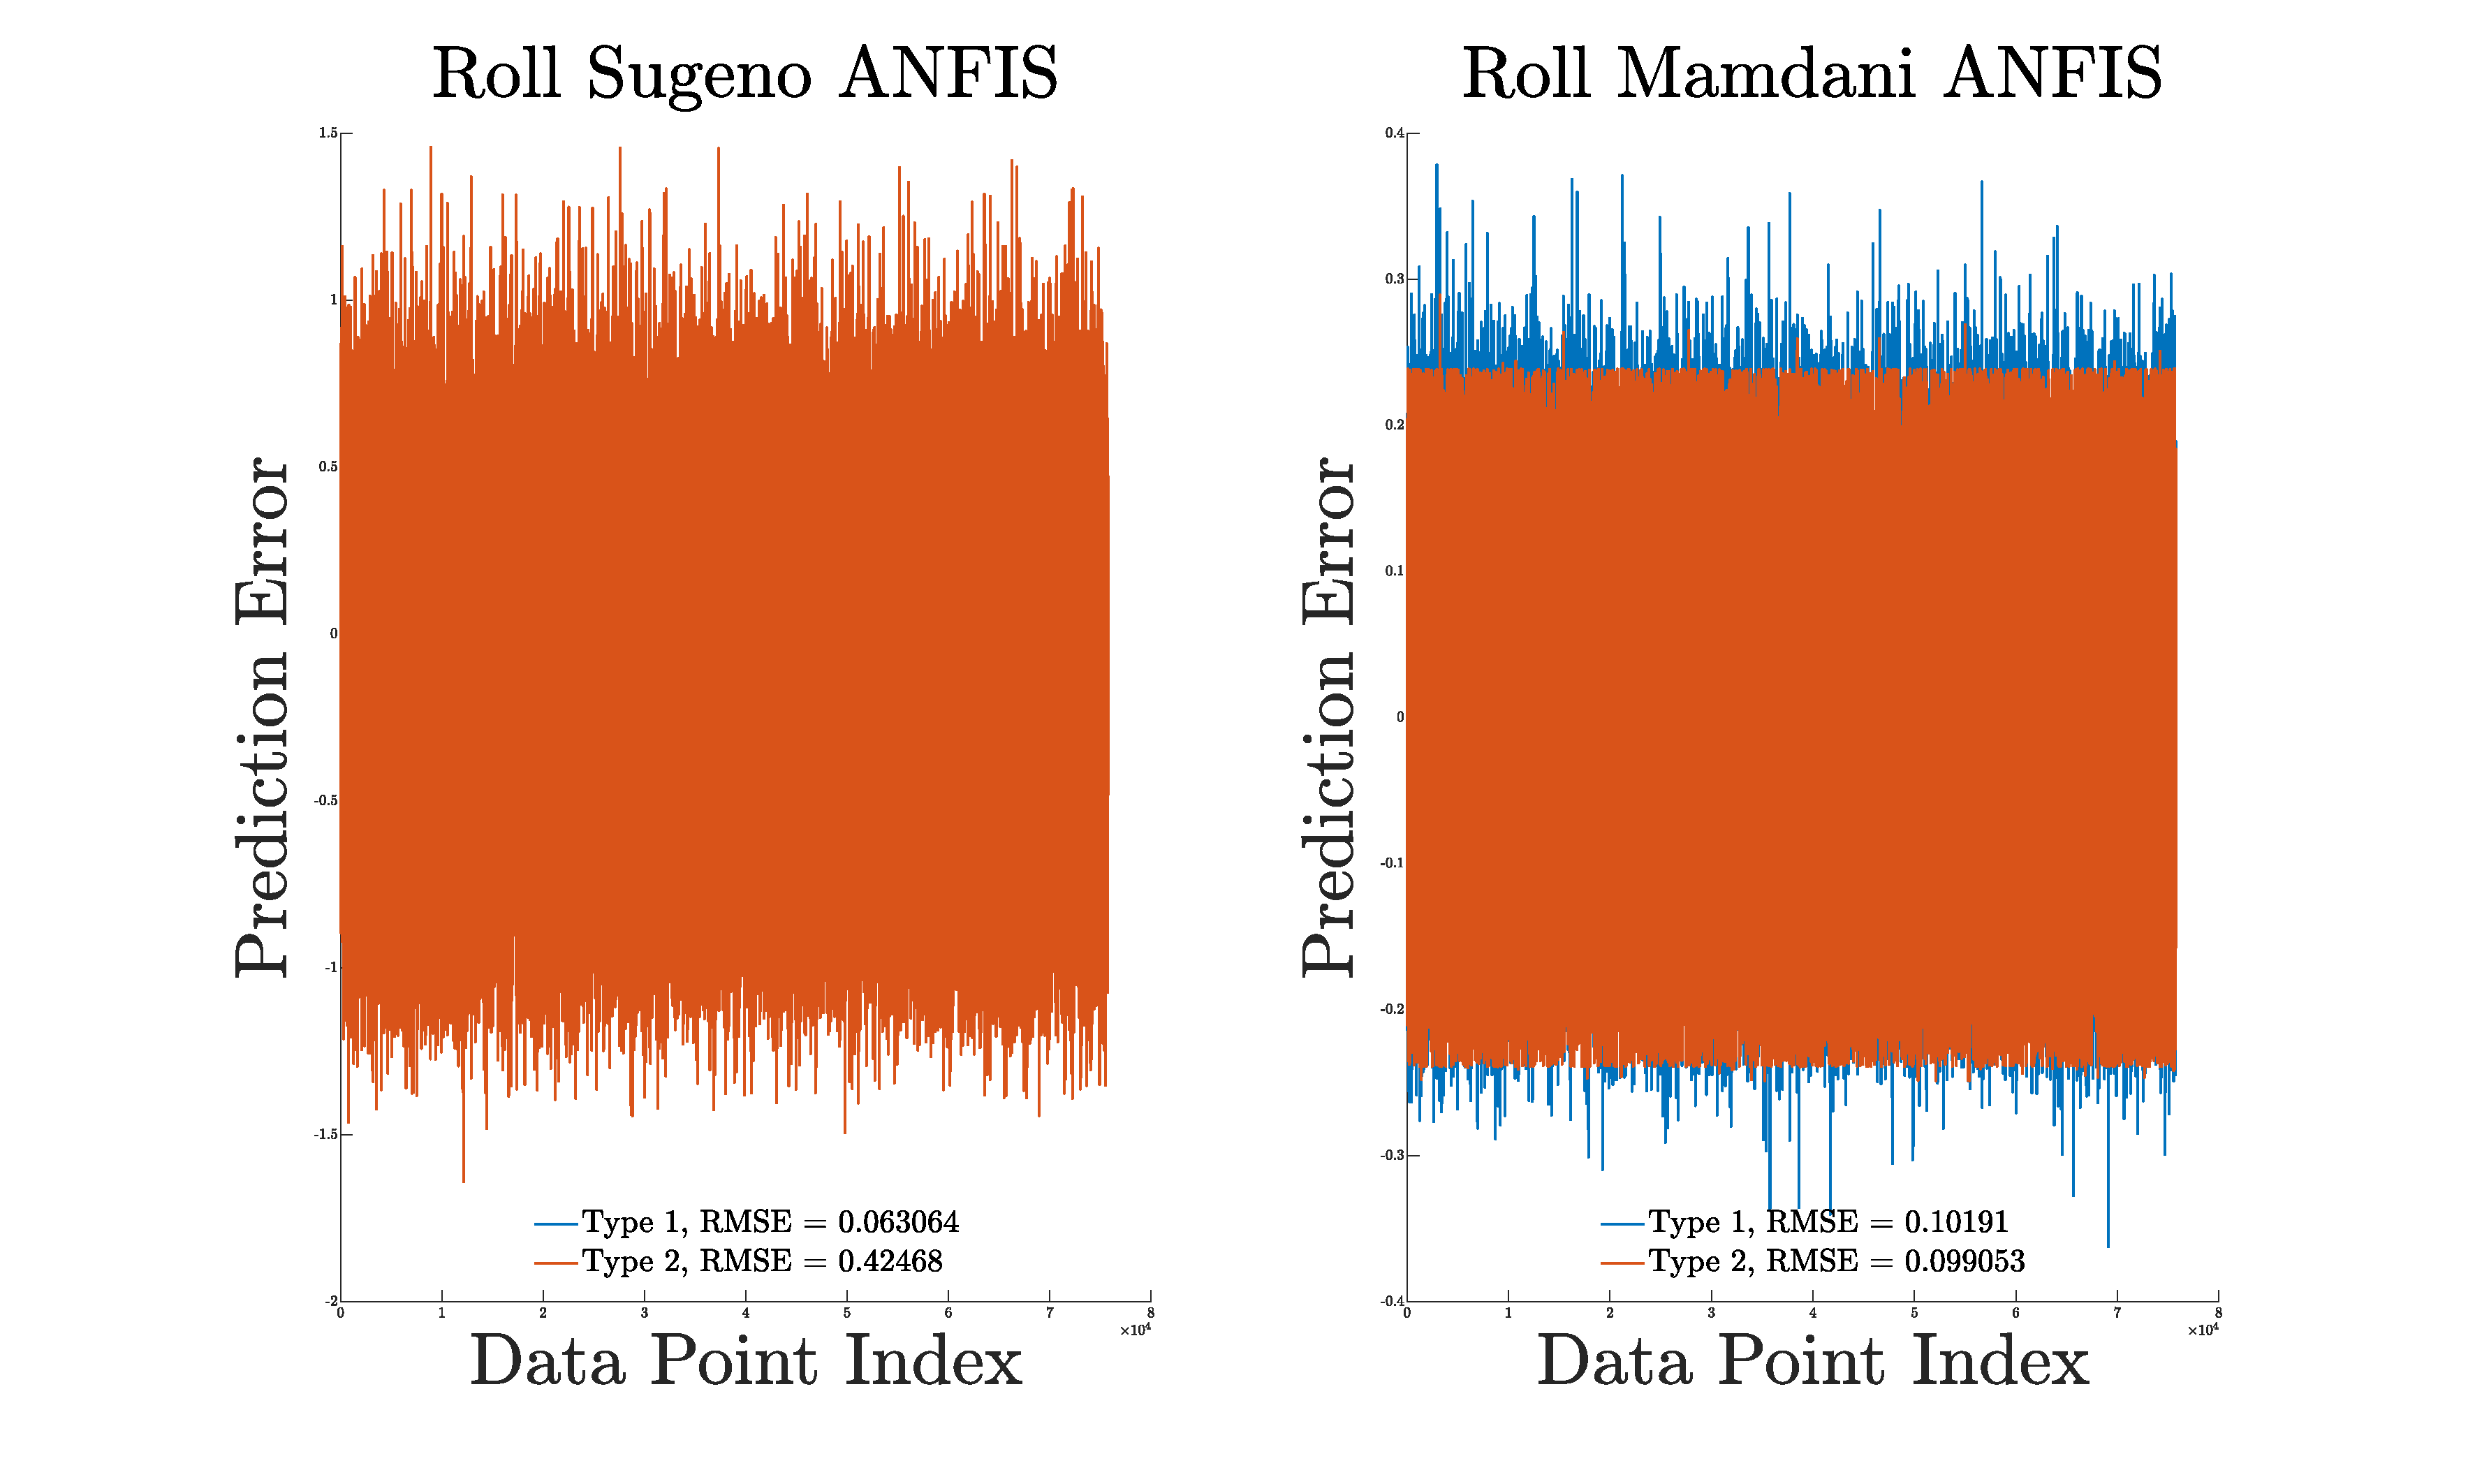
\includegraphics[width = 0.8\textwidth]{img/Roll Type.pdf}
    \caption{RMSE results for Type-1 and Type-2 Configurations for Roll Output}
    \label{fig:roll_type}
\end{figure}
\begin{figure}[H]
    \centering
    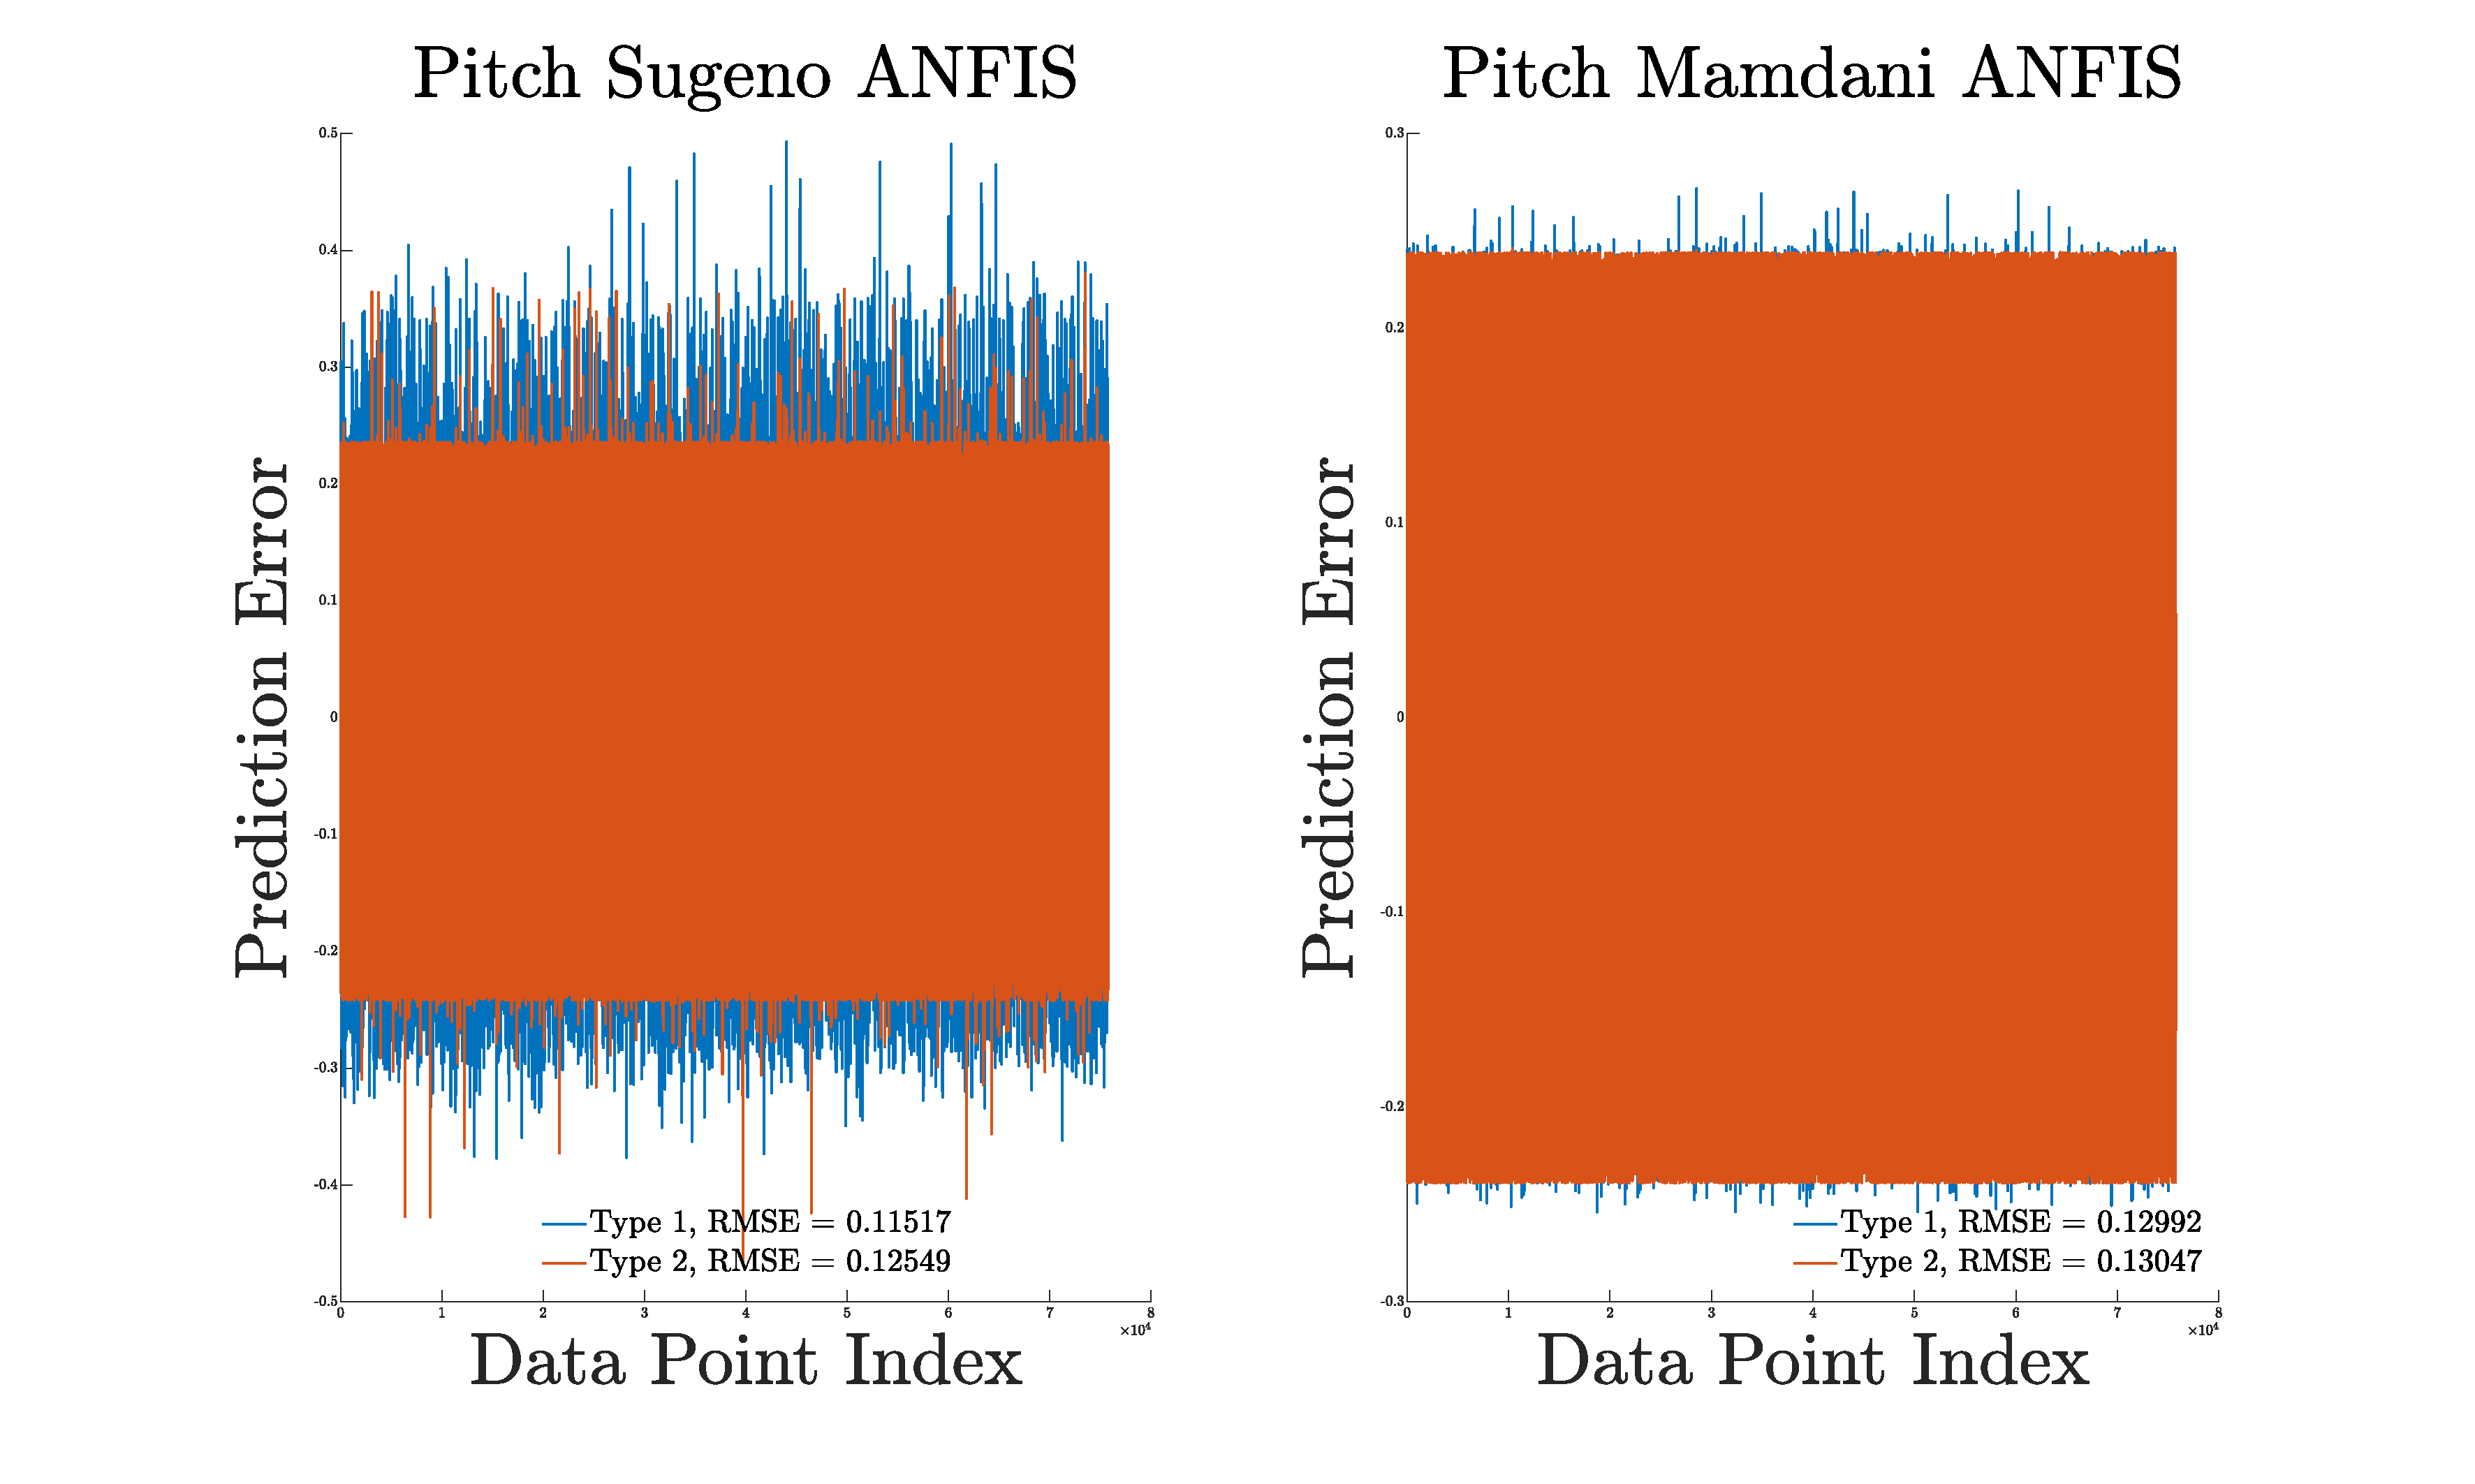
\includegraphics[width = 0.8\textwidth]{img/Pitch Type.pdf}
    \caption{RMSE results for Type-1 and Type-2 Configurations for Pitch Output}
    \label{fig:pitch_type}
\end{figure}
\begin{figure}[H]
    \centering
    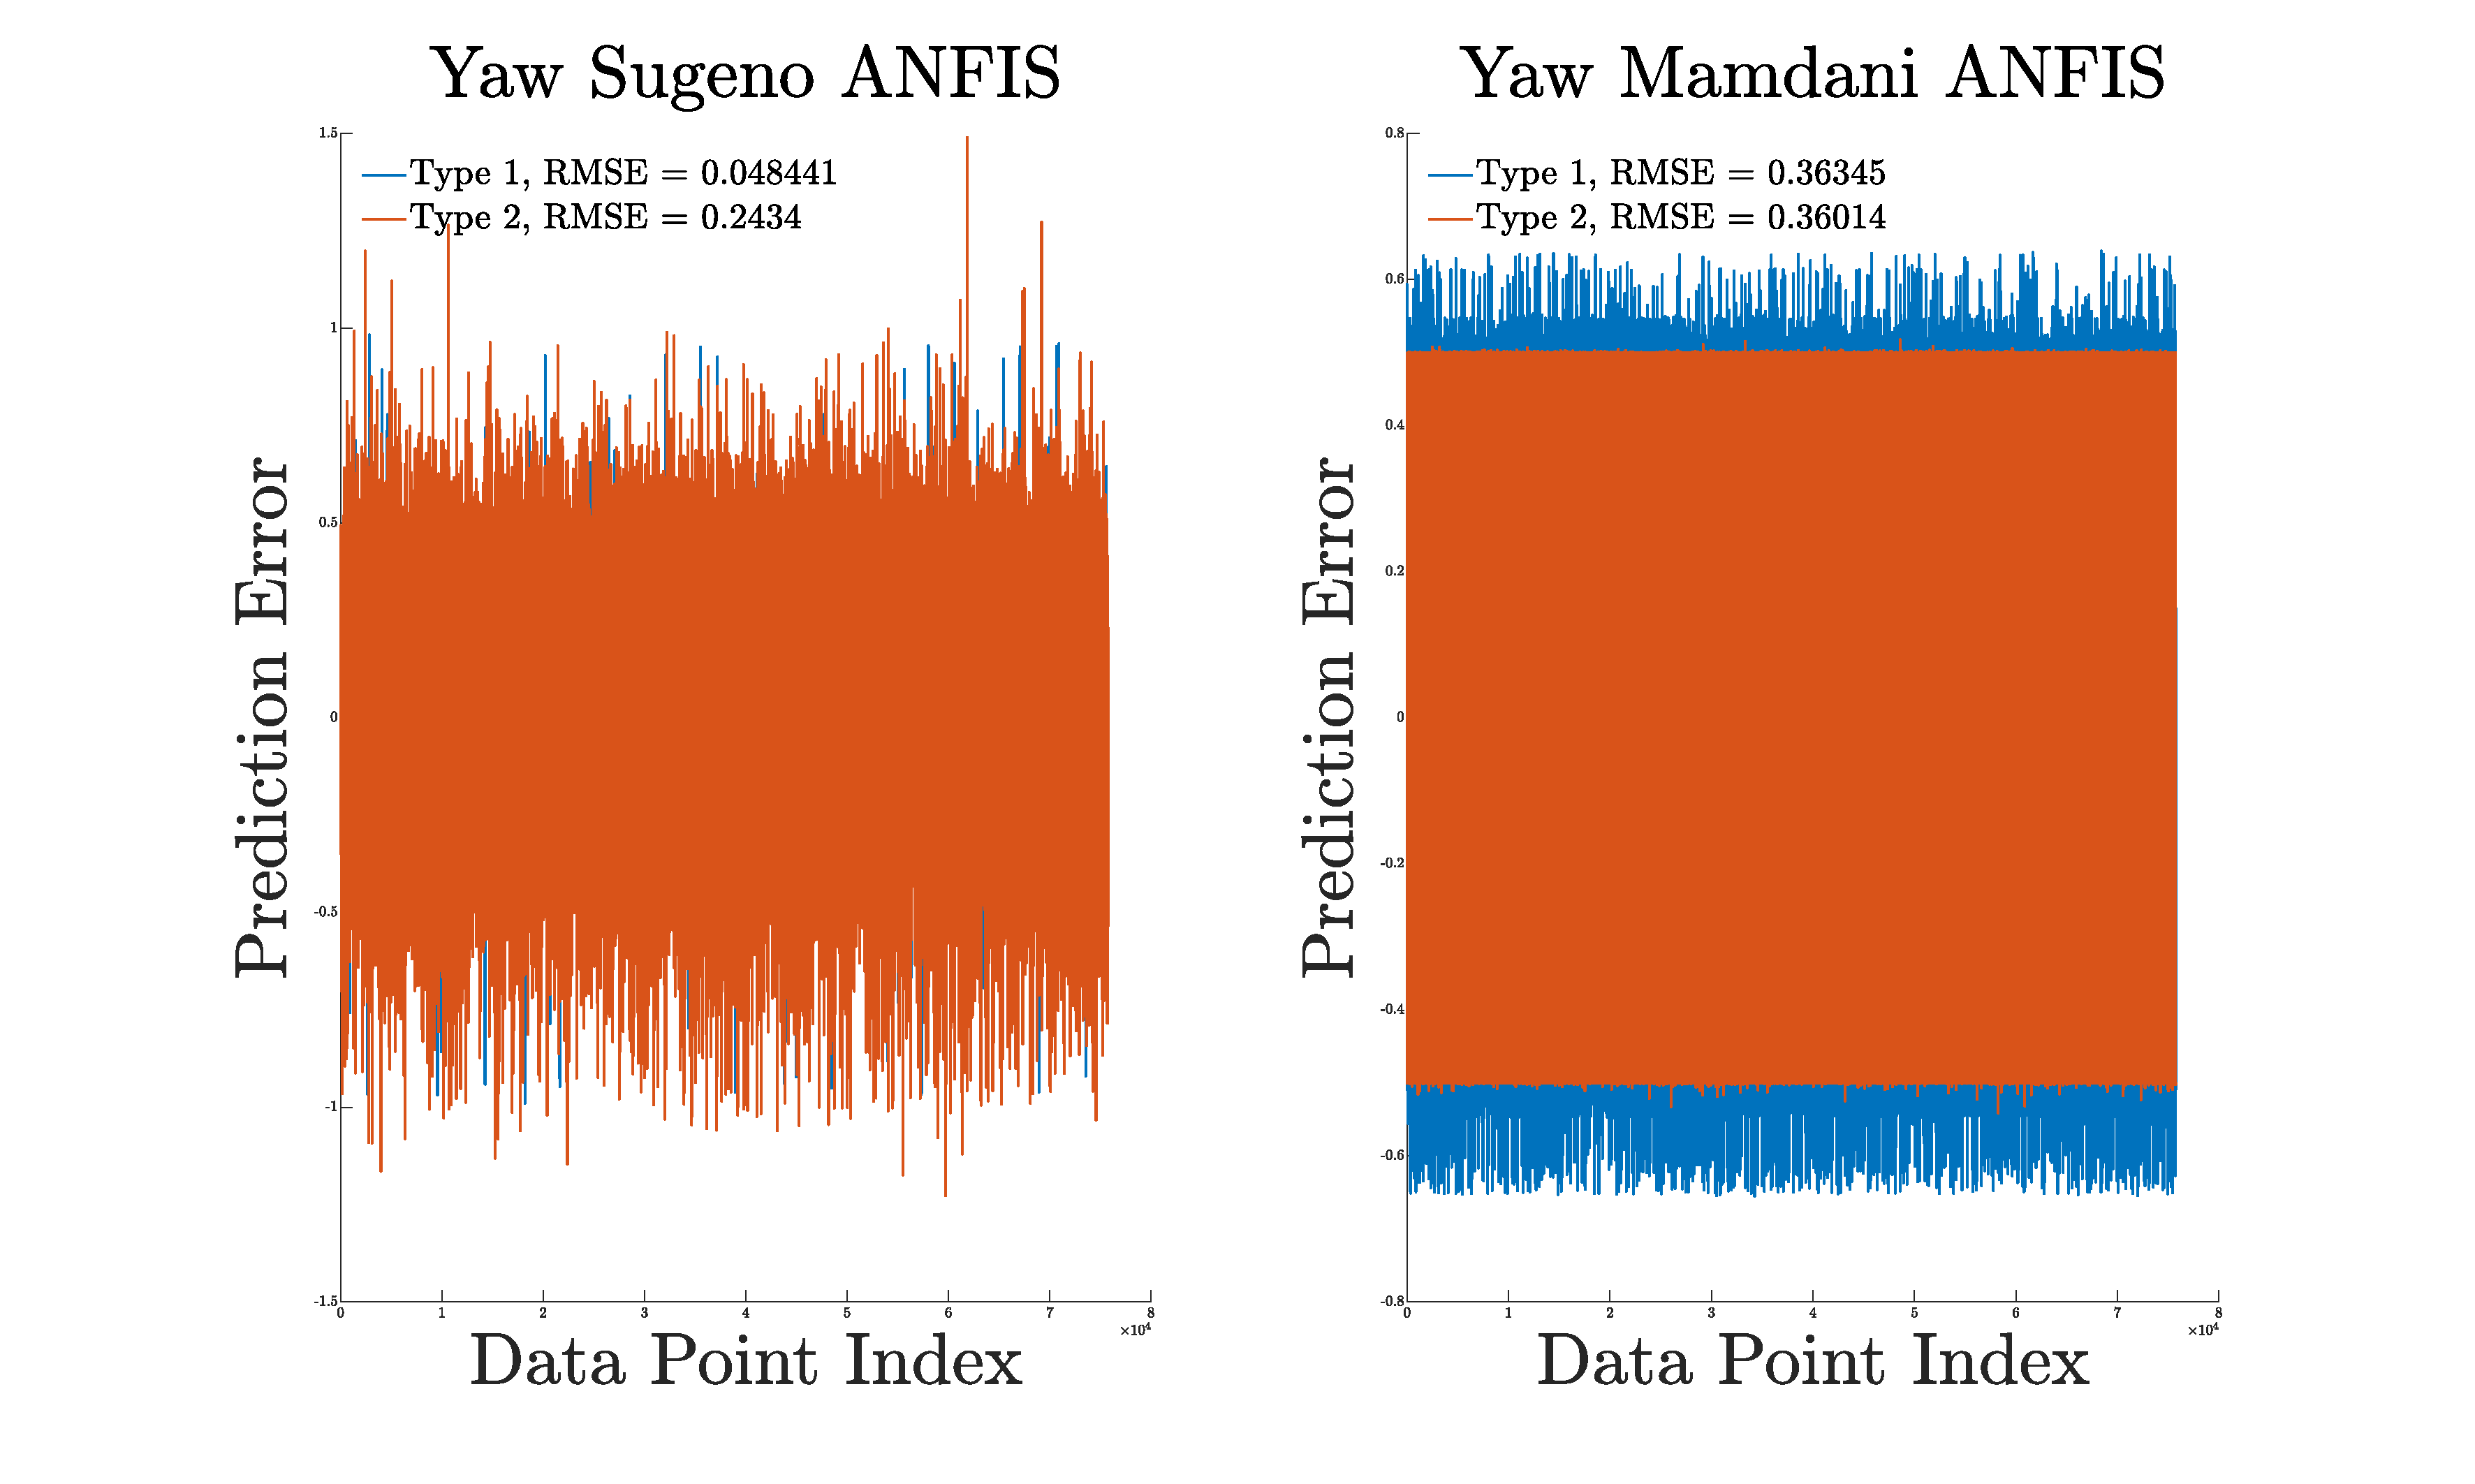
\includegraphics[width = 0.6\textwidth]{img/Yaw Type2.pdf}
    \caption{RMSE results for Type-1 and Type-2 Configurations for Yaw Output}
    \label{fig:yaw_type}
\end{figure}
\begin{figure}[H]
    \centering
    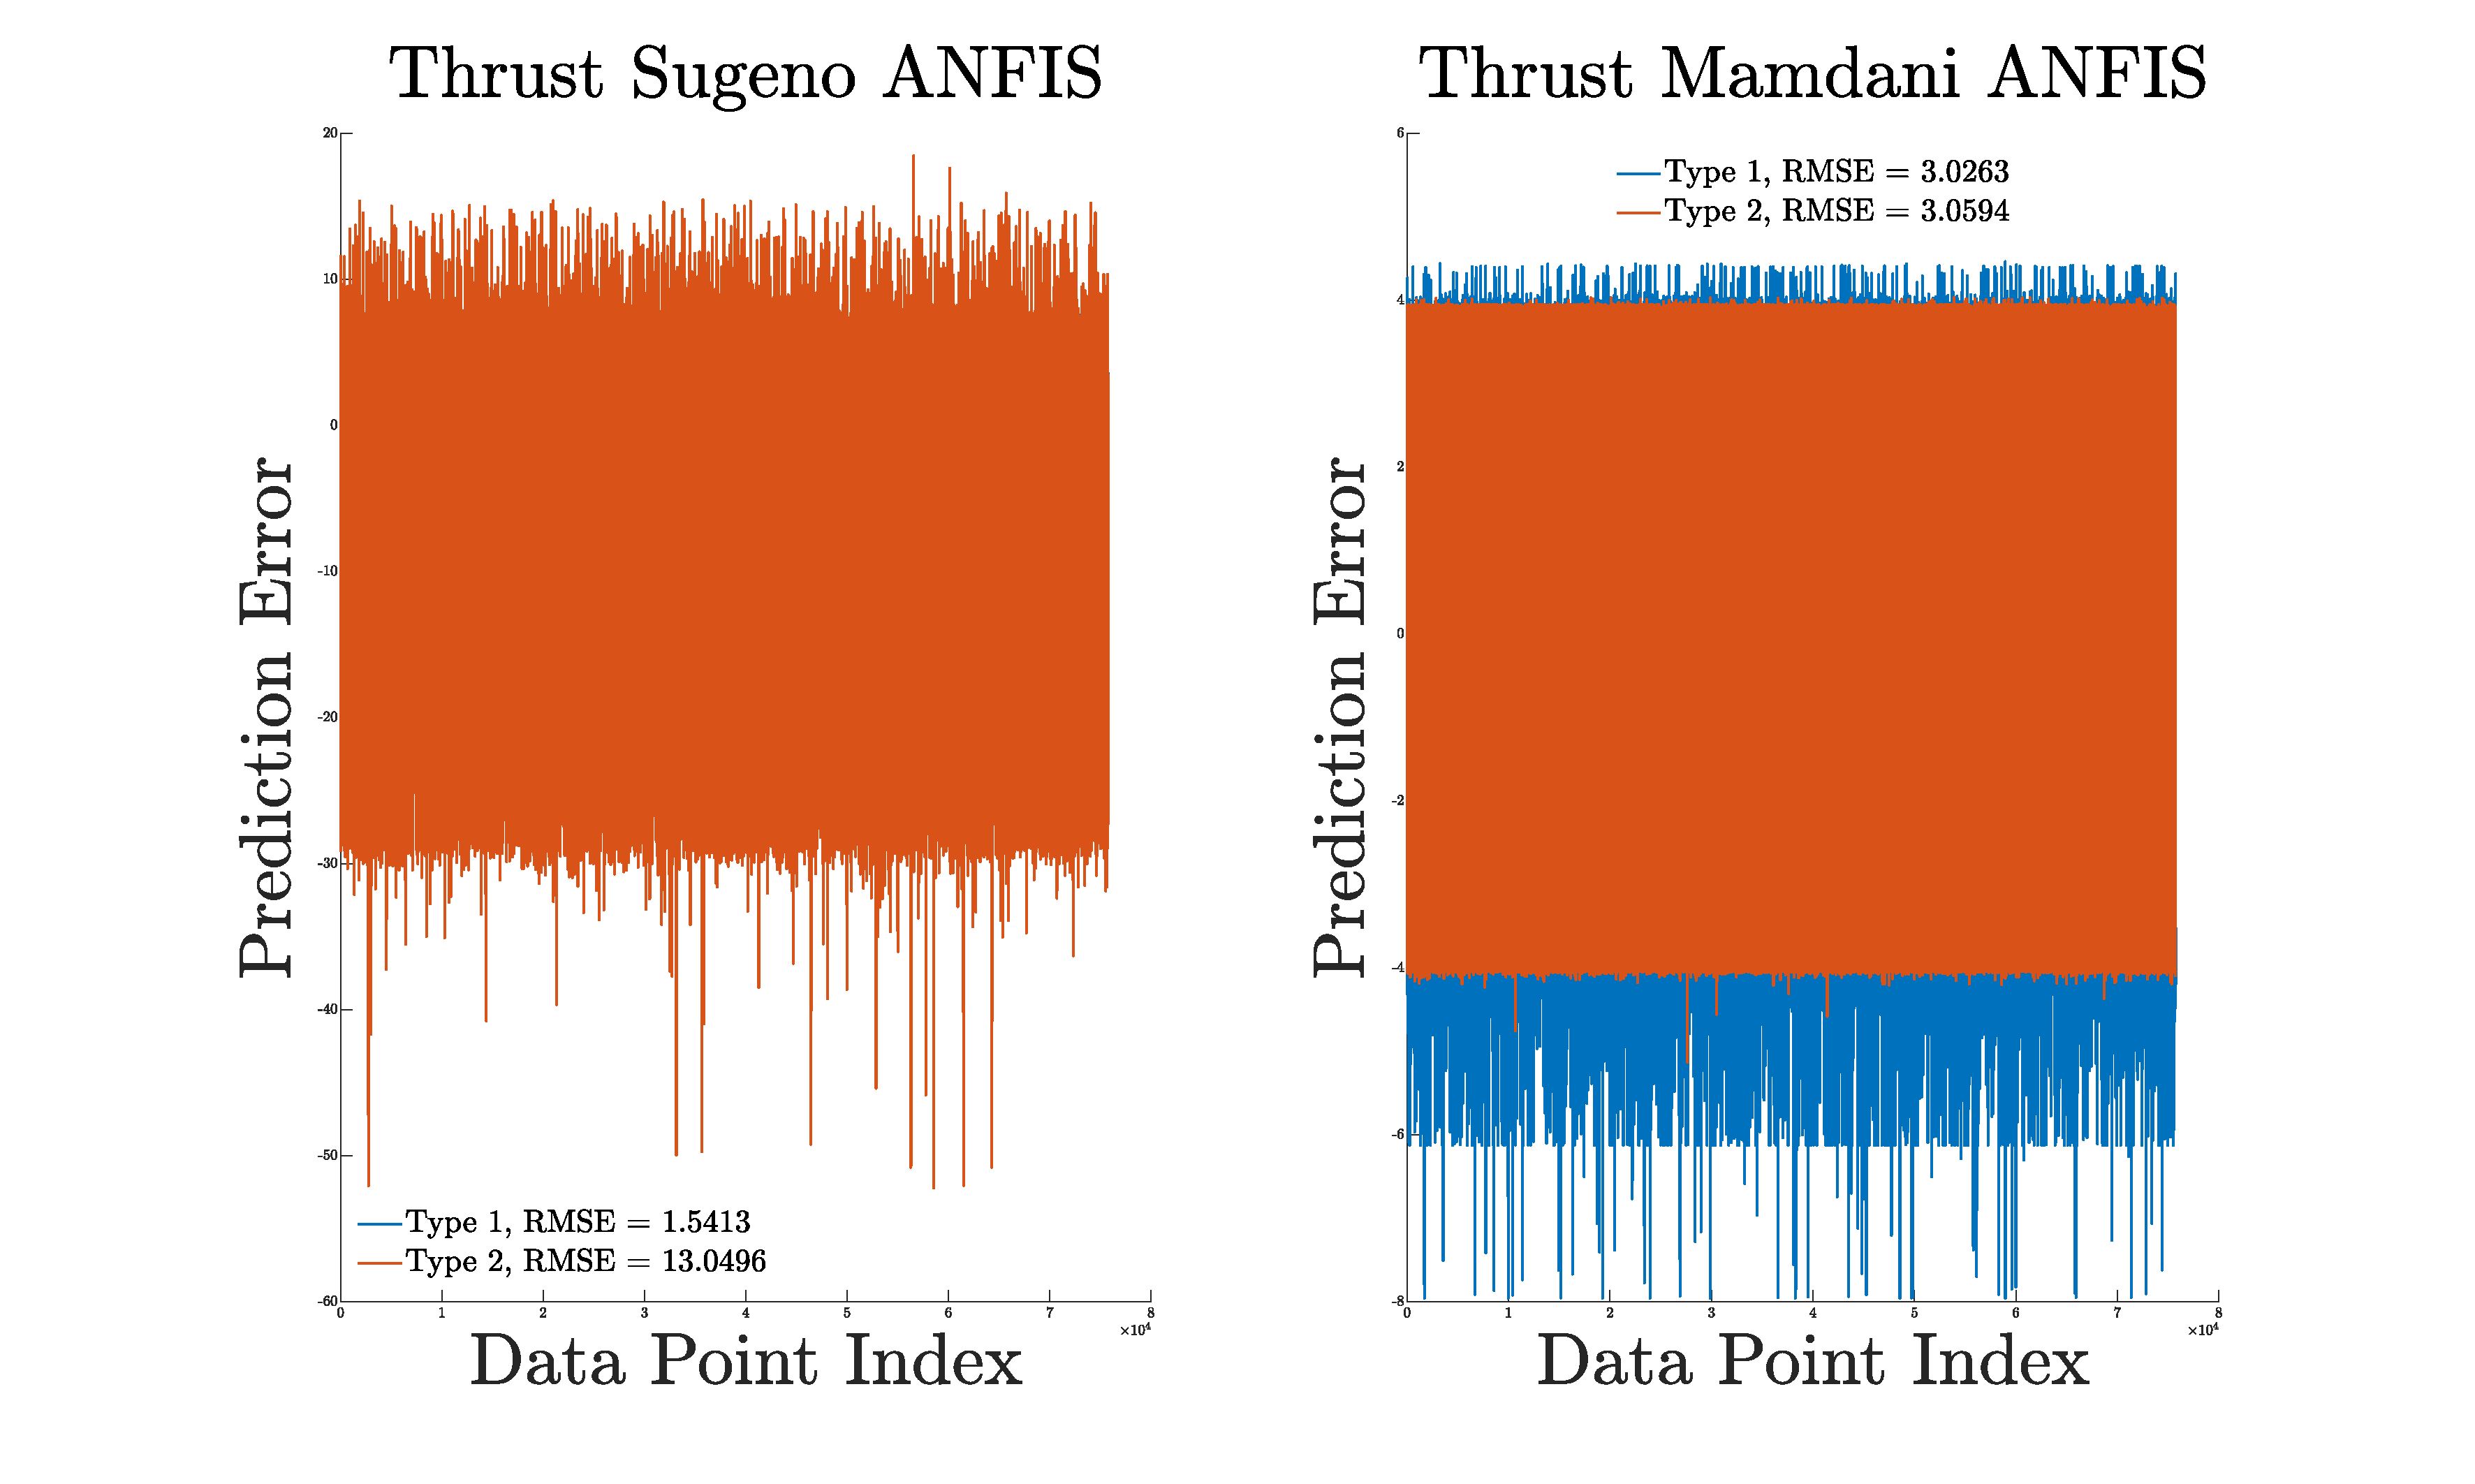
\includegraphics[width = 0.6\textwidth]{img/Thrust Type.pdf}
    \caption{RMSE results for Type-1 and Type-2 Configurations for Thrust Output}
    \label{fig:thrust_type}
\end{figure}
\begin{figure}[H]
    \centering
    \begin{minipage}[b]{0.45\textwidth}
        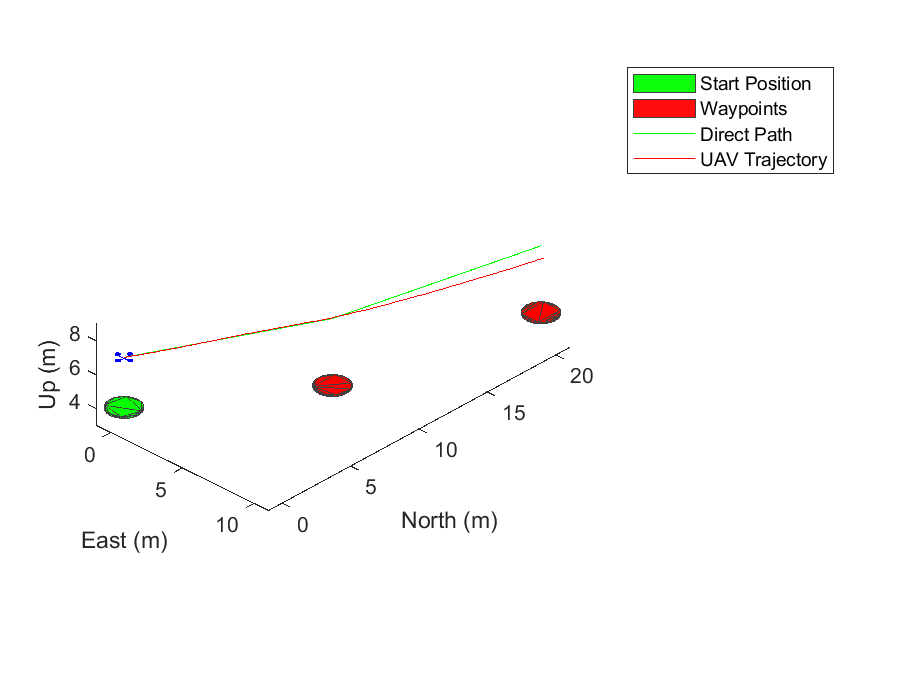
\includegraphics[height=5cm,keepaspectratio]{img/scenario1_pid_paths.eps}
        \caption{Scenario 1 Path taken using PID Drone Control}
        \label{fig:Paths1_pid}
    \end{minipage}
    \hfill
    \begin{minipage}[b]{0.45\textwidth}
        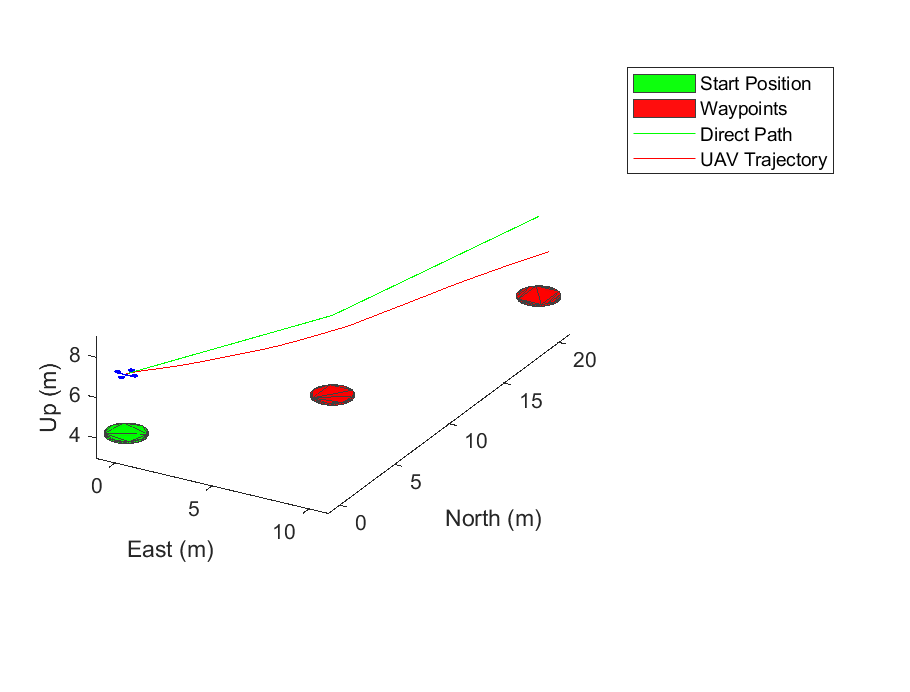
\includegraphics[height=5cm,keepaspectratio]{img/scenario1_fis_paths.eps}
        \caption{Scenario 1 Path taken using ANFIS Drone Control}
        \label{fig:Paths1_fis}
    \end{minipage}
\end{figure}
\begin{figure}[H]
    \centering
    \begin{minipage}[b]{0.45\textwidth}
        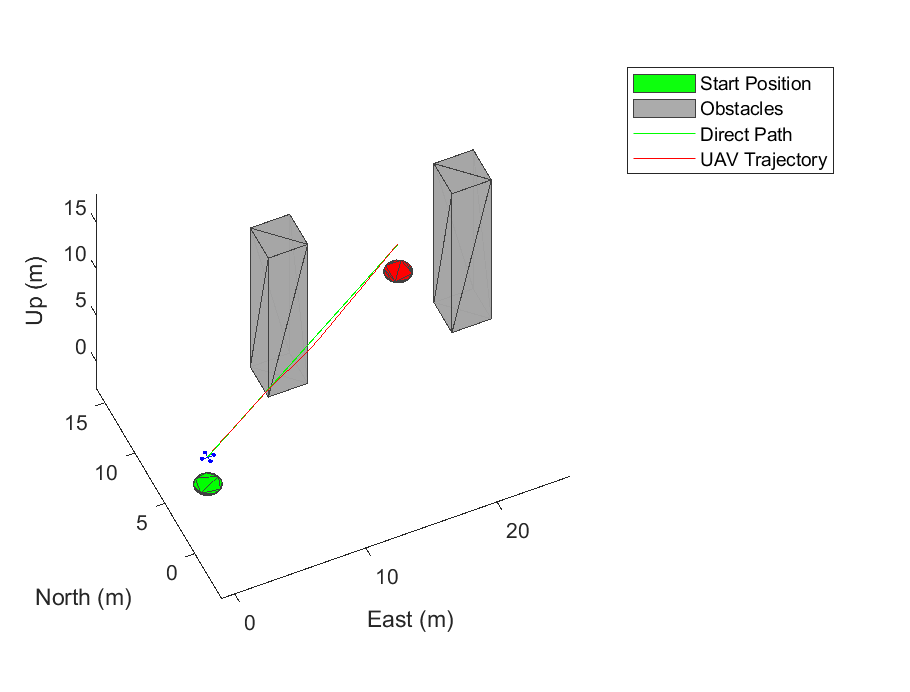
\includegraphics[height=5cm,keepaspectratio]{img/scenario2_pid_paths.eps}
        \caption{Scenario 2 Path taken using PID Drone Control}
        \label{fig:Paths2_pid}
    \end{minipage}
    \hfill
    \begin{minipage}[b]{0.45\textwidth}
        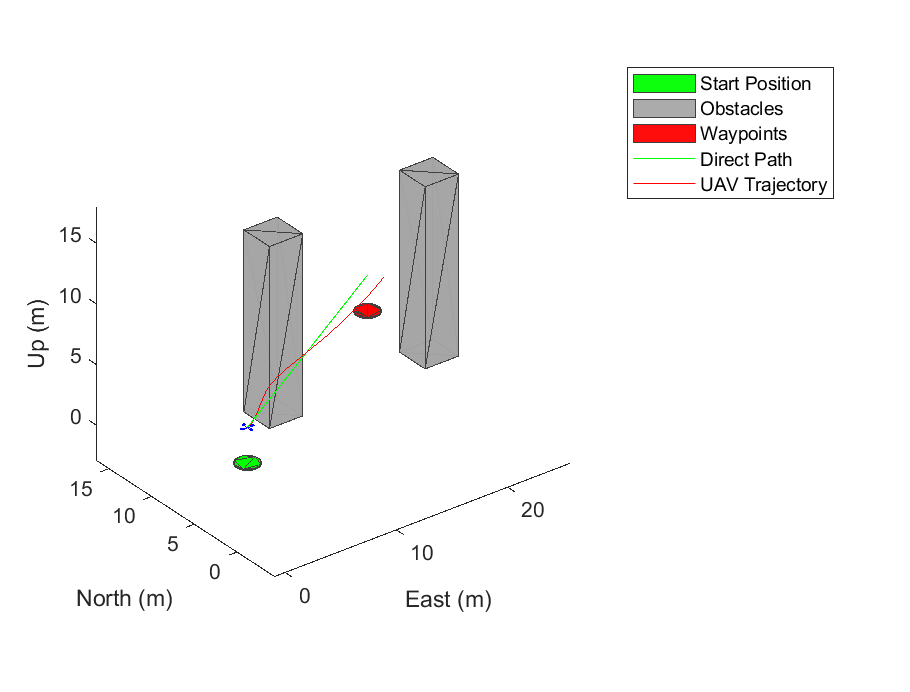
\includegraphics[height=5cm,keepaspectratio]{img/scenario2_fis_paths.eps}
        \caption{Scenario 2 Path taken using ANFIS Drone Control}
        \label{fig:Paths2_fis}
    \end{minipage}
\end{figure}
\begin{figure}[H]
    \centering
    \begin{minipage}[b]{0.45\textwidth}
        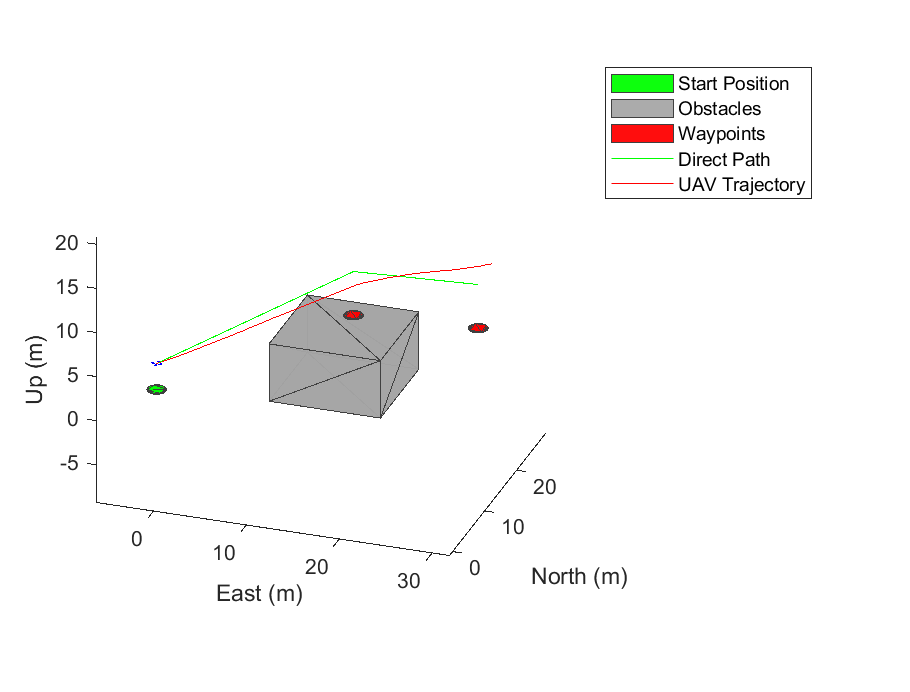
\includegraphics[height=5cm,keepaspectratio]{img/scenario3_pid_paths.eps}
        \caption{Scenario 3 Path taken using PID Drone Control}
        \label{fig:Paths3_pid}
    \end{minipage}
    \hfill
    \begin{minipage}[b]{0.45\textwidth}
        \includegraphics[height=5cm,keepaspectratio]{img/scenario3_fis_paths.eps}
        \caption{Scenario 3 Path taken using ANFIS Drone Control}
        \label{fig:Paths3_fis}
    \end{minipage}
\end{figure}
\begin{figure}[H]
    \centering
    \begin{minipage}[b]{0.45\textwidth}
        \includegraphics[height=5cm,keepaspectratio]{img/scenario4_pid_paths.eps}
        \caption{Scenario 4 Path taken using PID Drone Control}
        \label{fig:Paths4_pid}
    \end{minipage}
    \hfill
    \begin{minipage}[b]{0.45\textwidth}
        \includegraphics[height=5cm,keepaspectratio]{img/scenario4_fis_paths.eps}
        \caption{Scenario 4 Path taken using ANFIS Drone Control}
        \label{fig:Paths4_fis}
    \end{minipage}
\end{figure}
\begin{figure}[H]
    \centering
    \begin{minipage}[b]{0.45\textwidth}
        \includegraphics[height=5cm,keepaspectratio]{img/scenario5_pid_paths.eps}
        \caption{Scenario 5 Path taken using PID Drone Control}
        \label{fig:Paths5_pid}
    \end{minipage}
    \hfill
    \begin{minipage}[b]{0.45\textwidth}
        \includegraphics[height=5cm,keepaspectratio]{img/scenario5_fis_paths.eps}
        \caption{Scenario 5 Path taken using ANFIS Drone Control}
        \label{fig:Paths5_fis}
    \end{minipage}
\end{figure}

\end{document}